
%%%%%%%%%%%%%%%%%%%%%%%%%%%%%%%%%%%%%%%%%%%%%%%%%%
% Basic setup. Most papers should leave these options alone.
\documentclass[fleqn,usenatbib]{mnras}

\usepackage[T1]{fontenc}
\DeclareRobustCommand{\VAN}[3]{#2}
\let\VANthebibliography\thebibliography
\def\thebibliography{\DeclareRobustCommand{\VAN}[3]{##3}\VANthebibliography}

%%%%% AUTHORS - PLACE YOUR OWN PACKAGES HERE %%%%%
\usepackage{graphicx}	% Including figure files
\usepackage{amsmath}	% Advanced maths commands
\usepackage{amssymb}	% Extra maths symbols
\usepackage{xspace} 
\usepackage{xcolor}
\usepackage{upgreek}
\usepackage{CJK}
\usepackage{fontawesome}
\usepackage{gensymb}
\usepackage{multirow}
\usepackage{mathtools}
\usepackage{newtxtext,newtxmath}
\usepackage{tabularx}

%%%%% AUTHORS - PLACE YOUR OWN COMMANDS HERE %%%%%
\newcommand{\ToDo}[1]{\textbf{\textcolor{blue}{ToDo: #1}}}
\newcommand{\SB}[1]{{\textcolor{purple}{SB: #1}}}
\newcommand{\TB}[1]{{\textcolor{blue}{TB: #1}}}
\newcommand{\Gaia}{\textit{Gaia}\xspace} % \Gaia
\newcolumntype{C}{>{\centering\arraybackslash}X}

\newcommand{\nihaoRmax}{$20\,\mathrm{kpc}$}
\newcommand{\nihaoZmax}{$10\,\mathrm{kpc}$}
\newcommand{\nihaoAGEmax}{$0.5\,\mathrm{Gyr}$}


%%%%%%%%%%%%%%%%%%%%%%%%%%%%%%%%%%%%%%%%%%%%%%%%%%
%%%%%%%%%%%%%%%%%%% TITLE PAGE %%%%%%%%%%%%%%%%%%%

% Title of the paper, and the short title which is used in the headers.
% Keep the title short and informative.
\title[Radial metallicity gradients in NIHAO-UHD]{More than just a line: Shining light on the flattening radial metallicity gradient of a NIHAO-UHD Milky-Way analogue simulation}

% The list of authors, and the short list which is used in the headers.
% If you need two or more lines of authors, add an extra line using \newauthor
\author[S. Buder and T. Buck]{
S. Buder,$^{1,2}$\thanks{E-mail: sven.buder@anu.edu.au} and
T. Buck,$^{3,4}$
\\
% List of institutions
$^{1}$Research School of Astronomy \& Astrophysics, Australian National University, ACT 2611, Australia\\
$^{2}$Center of Excellence for Astrophysics in Three Dimensions (ASTRO-3D), Australia\\
$^{3}$Universit{\"a}t Heidelberg, Interdisziplin{\"a}res Zentrum f{\"u}r Wissenschaftliches Rechnen, Im Neuenheimer Feld 205, D-69120 Heidelberg, Germany\\
$^{4}$Universit{\"a}t Heidelberg, Zentrum f{\"u}r Astronomie, Institut f{\"u}r Theoretische Astrophysik, Albert-Ueberle-Straße 2, D-69120 Heidelberg, Germany
}

% These dates will be filled out by the publisher
\date{Accepted YYYY Month DD. Received YYYY Month DD}

% Enter the current year, for the copyright statements etc.
\pubyear{2024}

% Don't change these lines
\begin{document}
\label{firstpage}
\pagerange{\pageref{firstpage}--\pageref{lastpage}}
\maketitle

% Abstract of the paper
\begin{abstract} % XXX words
% Context
Radial metallicity gradients in galaxies are crucial for understanding the processes of galaxy formation and its dynamical and chemical evolution.
% Method
We use young stars and gas of a high-resolution simulation of a NIHAO-UHD Milky Way analogue galaxy to analyse four properties of the radial metallicity gradient, namely its linearity and scatter as well as its coherence with radial coverage, azimuth, and age.
% Results
While a global linear fit with slope traces the gradient well, we find it to be too flat in the inner galaxy and too steep in the outer galaxy. An initially stepper but then flattening second order quadratic function provides a superior fit down to the smallest radial steps, where less regular effects take over. We identify these as \SB{spiral arms or warp?} when tracing them across the Galactic position. The simulation further exhibits a steadily increasing spread in [Fe/H] even among the young stars from 0.01 dex in the inner galaxy to 0.14 dex at a radius 20 kpc coinciding with decreasing stellar density and increased flaring of stars towards higher heights with little correlation across the small age range of 1 Gyr.
% Conculsions
We conclude that future Galactic and extragalactic observational studies should test our theoretical prediction of a quadratic gradient function with their data to confirm or reject previous observational claims of a broken linear radial metallicity gradient proposed for the Milky Way and other spiral galaxies, as either function implies different dynamical and chemical galaxy formation and evolution scenarios.
\end{abstract}
% Select between one and six entries from the list of approved keywords.
% Don't make up new ones.
\begin{keywords}
cosmology: observations -- Galaxy: structure -- Galaxy: abundances  -- galaxies: structure -- galaxies: abundances
\end{keywords}

%%%%%%%%%%%%%%%%%%%%%%%%%%%%%%%%%%%%%%%%%%%%%%%%%%

%%%%%%%%%%%%%%%%% BODY OF PAPER %%%%%%%%%%%%%%%%%%

\section{Introduction}
\label{sec:intro}

Radial metallicity gradients in galaxies, defined as the change in metal abundance with galactocentric radius, offer vital insights into the processes that shape the chemical and dynamical evolution of galaxies. The decrease in metallicity with increasing distance from the Galactic center is well-established both theoretically \citep{Larson1976, Tinsley1980, Chiosi1980} and observationally in the Milky Way \citep{Searle1971, Janes1979, Twarog1997}. However, the specific shape and characteristics of this gradient remain somewhat unclear. \SB{sentence about connecting MW with extragalactic... (to not lose the readers)}

The Milky Way, being the only galaxy where we can resolve millions of stars, provides a unique opportunity to study these gradients in detail. Over two decades ago, \citet{Chiappini2002} highlighted the contradictions in the observed shape, magnitude, and evolution of abundance gradients. Recent advancements, such as the \textit{Gaia} mission \citep{Gaia-Collaboration2016}, have significantly expanded our observational data, allowing for more detailed studies of these gradients.

For instance, \citet{Hogg2019} created an extensive metallicity map of the Milky Way using APOGEE and \textit{Gaia} data, while \citet{Poggio2022} mapped young stars and found a metallicity excess around spiral arms \citep[see also][]{Zari2018, Zari2021, Poggio2021, Hackshaw2024}. Similarly, \citet[][among others]{Imig2023} traced gradients across different stellar populations and ages, emphasizing the importance of considering radial migration effects \citep{Binney2008, Frankel2018, Frankel2020}.

Historically, radial metallicity gradients have been measured using various stellar populations and gas tracers. Early evidence by \citet{Janes1979} suggested a gradient on the order of
\begin{equation}
\frac{\mathrm{d{[Fe/H]}}}{\mathrm{d}R} = -0.05 \pm 0.01,\mathrm{dex,kpc^{-1}}
\end{equation}
for the Milky Way which aligns with more recent measurements \citep{Anders2017, Hayden2015}. Estimated gradients also seem to be broadly consistent across different stellar tracers, such as young open clusters \citep[e.g.][]{Yong2012, Cunha2016, Magrini2017, Casamiquela2019, Donor2020, Spina2021,Myers2022}, young hot (OB-type) stars \citep{Zari2018, Zari2021, Poggio2021, Poggio2022}, field stars close to the Galactic plane \citep[e.g.][]{Bergemann2014} or Cepheids \citep{Andrievsky2002, Andrievsky2002b, Lemasle2007, Lemasle2013}. However, these gradients are accompanied by significant spread in [Fe/H] of $0.1-0.15\,\mathrm{dex}$, as noted by \citet{Twarog1980}, which may imply a fine structure of the metallicity gradient \citep[see][]{Genovali2014}.

Despite extensive observational efforts, several challenges persist:
\begin{itemize}
    \item The completeness (or patchiness) of observed datasets remains a fundamental issue \citep{Bergemann2014}.
    \item How robustly can we use the incomplete data to predict substructure in the gradients, such as the need to actually fit two linear gradients with a break radius at corotation radius \citep[][and references therein]{Bresolin2012} or further out \citep{Yong2012, Donor2020} - or even more complicated functions \citep[see e.g.][]{Chiappini2001, Kubryk2015}?
    \item Different samples yield varying gradients, potentially due to biases in data or the inclusion of older stars \citep[e.g.][]{Boeche2013, AllendePrieto2006, Katz2011, Hayden2014, Anders2014, Vickers2021, Willett2023}.
    \item The impact of spiral arm structures \citep{Poggio2021}, the Galactic warp \citep{Lemasle2022} or bar-driven mixing \citep{DiMatteo2013} on metallicity gradients is not fully understood.
    \item Methodologies for fitting linear models to scattered data need re-evaluation \citep{Metha2021}.
\end{itemize}

Understanding these gradients in the Milky Way is also crucial for extragalactic studies, where spatial resolution limits observations. New instruments like the MUSE integral field spectrograph have enabled a plethora of extragalactic studies to contrast the Milky Way to and techniques like the spectroscopy of HII regions and planetary nebulae have helped to infer gas metallicity distributions in external galaxies \citep{Shaver1983, Vilchez1996, Rolleston2000, Bresolin2012}. Recent examples include \citet{Sanchez2014} with CALIFA galaxy observations as well as \citet{Mun2024} and \citet{Chen2024} who use MAGPI galaxy observations to probe for example the effects of spiral arms. Notable is also the scatter that \citet{Chen2023} found for the gas metallicity across galactic radius with TYPHOON observations (see their. Figs. 4-6). \SB{\citet{Grasha2022} suggested that the flattening of the gas metallicity in their TYPHOON galaxies could be caused by changes in the ratio of supernovae II and AGB reflected by a changing ratio of nitrogen to oxygen abundance N/O which also flattens towards a lower plateau below metallicities of $A(O) \sim 8.0$ \citep{Nicholls2017}.}

\SB{Look into I-Ting's work: \citet{Ho2015, Ho2017c, Ho2018, Ho2019}}
\SB{Look into Sharon's work: \citet{Meidt2008, Meidt2009}}

From a modelling perspective, galactic chemical evolution models can both test understanding of radial metallicity gradients and make predictions beyond the limited volumes and tracers tested by Milky Way and extragalactic studies. Such galactic chemical evolution models include \citet{Chiappini2001, Matteucci2001b, Minchev2014b, Kubryk2015, Stanghellini2015, Rybizki2017}. \citet{Sharda2021} even presented a model for gas phase metallicity gradients in galaxies and their evolution from first principles.

New suites of large-scale simulations now allow to gain insights into radial metallicity gradients across a range of simulated galaxies - including Milky Way analogues. While \citet{Pilkington2012} found that such gradients are established by inside-out formation in RaDES simulations, whereas \citet{Tissera2019} used EAGLE simulations to study gradients across different galaxy characteristics, such as mergers and stellar mass. \citet{Bellardini2021} and \citet{Bellardini2022, Graf2024} compared the radial metallicity gradient and its azimuthal scatter for different simulations of the FIRE suite for gas and stars, respectively. Focusing on the change of the radial metallicity gradient over time, \citet{Grand2015} assessed the scatter of radial metallicity distribution for different stellar ages. \citet{Grand2016} looked at stars with ages below $3\,\mathrm{Gyr}$ in AURIGA and linked deviations from a global gradient towards slightly lower and higher metallicities with the leading and trailing edges of spiral arms, respectively. \citet{Grand2016} even found significant changes to the metallicity induced during $120\,\mathrm{Myr}$, or roughly one galactic rotation. Both \citet[][see their Fig. 6]{Ma2017} with FIRE and \citet[see their Fig. 9][]{Agertz2021} with VINTERGATAN further assessed the evolution of the radial metallicity gradient for gas and stars. \citet{Buck2023} studied how the gas metallicity gradient changes over time in the NIHAO-UHD simulations and found periods of time where the gradient surprisingly steepens. This finding resembles closely the findings of \citet{Lu2022} and \citet{Ratcliffe2023} for the Milky Way. This steepening phase could be connected and explained by major accretion events in the simulations. \citet{Khoperskov2023e} again focused on the gas and found the scatter of the gas metallicity of $\approx 0.04-0.06\,\mathrm{dex}$ at a given galactocentric distance. \SB{\citet{Hemler2021} evolution of the gas-phase radial metallicity gradient with redshift and galaxy mass in IllustrisTNG and \citet{Garcia2023} studied the }

This study here aims to advance these theoretical insight by addressing four critical scientific questions using a high-resolution simulation of a Milky Way analogue galaxy focussing on the inner $R_\mathrm{Gal.} \leq 20\,\mathrm{kpc}$:
\begin{enumerate}
\item \textit{Linearity of the gradient:} Assess the extent to which the radial metallicity gradient of young stars is linear.
\item \textit{Scatter in the gradient:} Quantify the expected scatter in the radial metallicity gradient of young stars.
\item \textit{Coherence of the gradient with position:} Investigate the gradient's variation with radial coverage and azimuth.
\item \textit{Coherence of the gradient with age:} Determine the reliability of stars as tracers of the gas disk over different ages.
\end{enumerate}

The paper is structured as follows: Section~\ref{sec:data} describes the data of our Milky Way analogue NIHAO-UHD simulation. Section~\ref{sec:linear_radial_metallicity_gradients} analyses the linearity of the radial metallicity gradient of the simulation, the first of our four objectives. Section~\ref{sec:scatter_radial_metallicity_gradients} then analyses both the scatter and local deviations from the gradient as well as the coherence of the gradient with vertical and azimuthal position as well as age (the remaining three objectives). Section~\ref{sec:discussion} discusses them individually. We note that in this research we are mainly interested in the specific shape of the radial metallicity gradient for radii relevant to Galactic observations. However, we also discuss our results in the context of extragalactic results that probe beyond the inner $20\,\mathrm{kpc}$ of a galaxy. Section~\ref{sec:conc} bundles our results into an overarching conclusion. 

\section{Data: A NIHAO-UHD Milky Way analogue simulation} \label{sec:data}

For this project, we use a cosmological zoom-in simulation of a Milky Way analogue (\texttt{g8.26e11}) from the \textit{Numerical Investigation of a Hundred Astronomical Objects} \citep[NIHAO,][]{Wang2015} project. The model galaxy has a virial radius of $R_{\rm vir}=206$ kpc and a total mass (gas, stars and dark matter) inside $R_{\rm vir}$ of $9.1 \cdot 10^{11}\,\mathrm{M_\odot}$. At redshift zero, it contains $8.2 \cdot 10^{11}\,\mathrm{M_\odot}$ dark matter, $6.4 \cdot 10^{10}\,\mathrm{M_\odot}$ gas mass and $2.3 \cdot 10^{10}\,\mathrm{M_\odot}$ stellar mass with a stellar mass resolution of around $7.5 \cdot 10^{3}\,\mathrm{M_\odot}$. This model galaxy was calculated as part of the NIHAO-UHD project \citep{Buck2020b} and has previously been used in various works studying Milky Way satellites \citep{Buck2019b}, Milky Way's dark halo spin \citep{Obreja2022} or inferring birth properties of stars with abundance clustering \citep{Ratcliffe2022}.

Simulations were carried out with the smoothed particle hydrodynamics code \texttt{Gasoline2} \citep{Wadsley2017} using cosmological parameters from \citet{Planck2014} with initial conditions and energetic feedback descriptions from the NIHAO project \citep{Wang2015}. Zoom-in simulations were then performed as described in detail by \citet{Buck2021} with star formation following \citet{Stinson2006} and energetic feedback following \citet{Stinson2013}. We note that this is a slightly different rerun of the same simulation than the one studied by \citet{Buder2024}. Here we are dealing with a higher resolution version and updated chemical yields.

\begin{figure*}
    \centering
    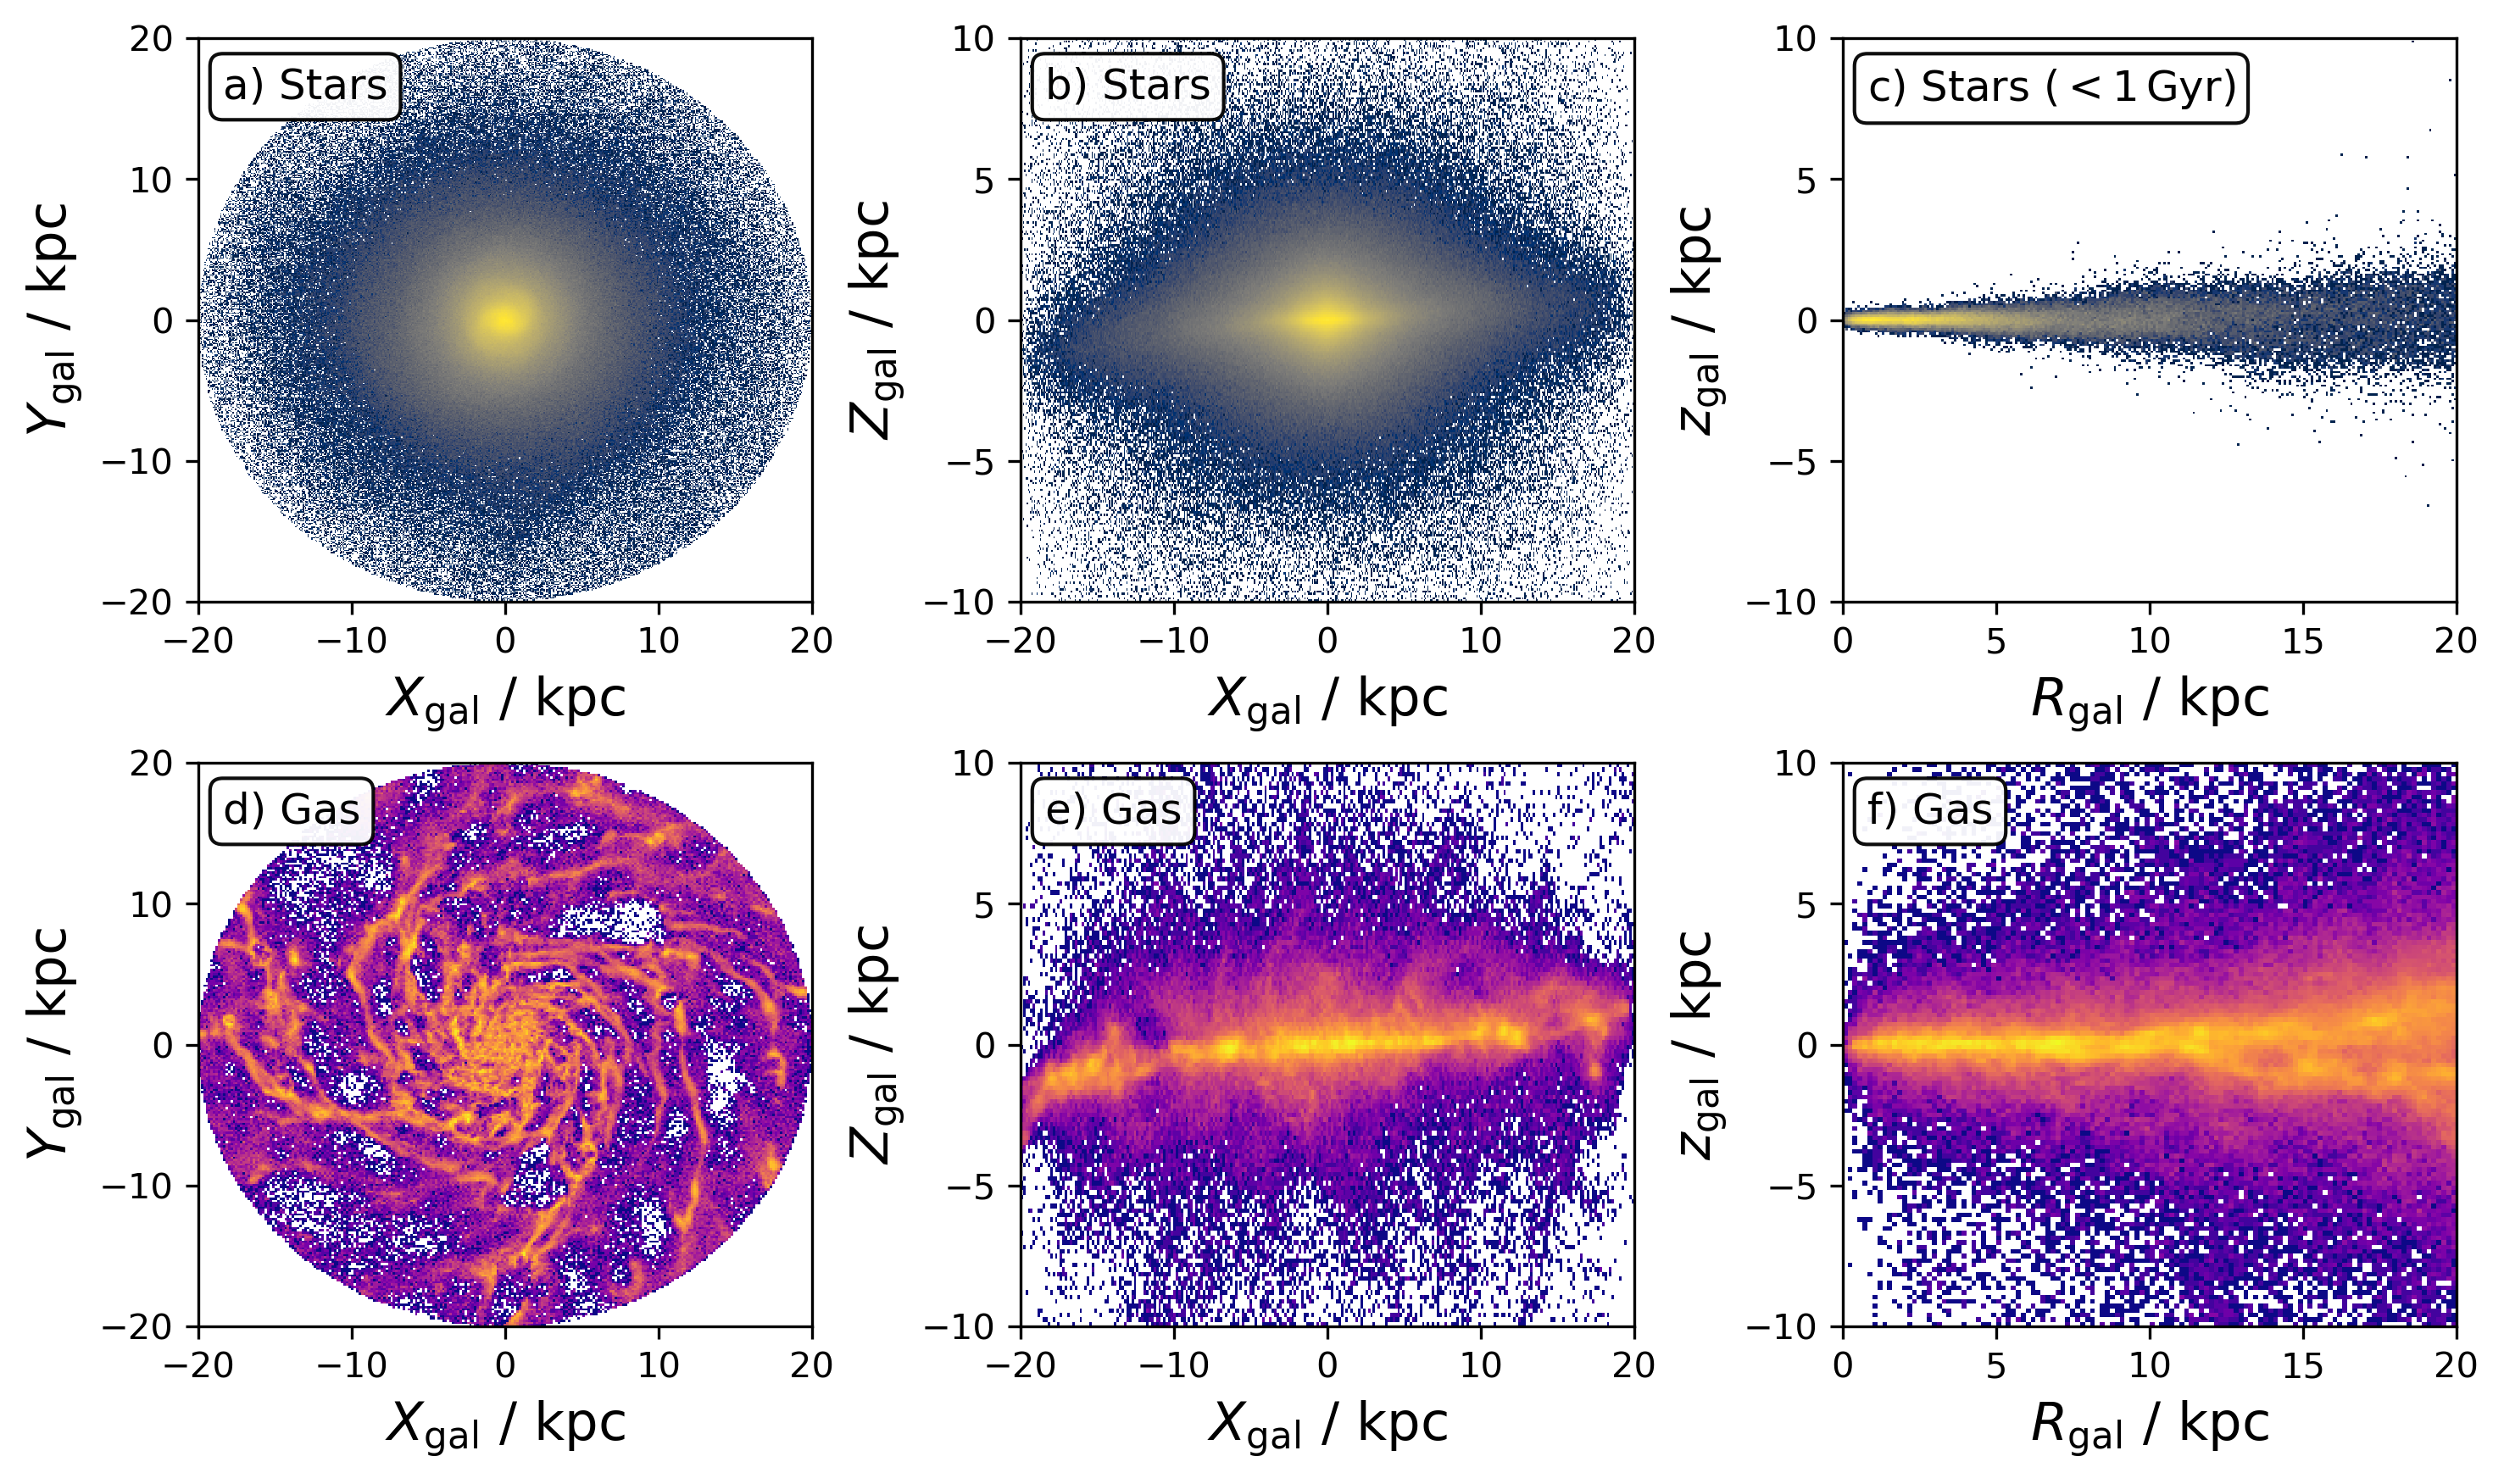
\includegraphics[width=\textwidth]{figures/stars_and_gas_overview.png}
    \caption{Logarithmic spatial density distribution of stars (upper panels) and gas (lower panels) within $R < 20\,\mathrm{kpc}$ of the NIHAO-UHD Milky Way analogue \texttt{g8.26e11} in galactocentric cartesian and cylindrical coordinates. Panel c) shows the influence of selecting only young stars with ages below \nihaoAGEmax.}
    \label{fig:stars_and_gas_overview}
\end{figure*}


Because computational resources still limit the mass resolution of simulations, we are relying on tracer particles that represent simple stellar populations (SSPs) with the same age, overall metallicity and discrete initial mass function (IMF). \citet{Buck2021} have implemented the flexible chemical evolution code \textsc{chempy} \citep{Rybizki2017} to calculate the chemical yields for the SSPs. In particular, we use the alternative (\texttt{alt}) setup of \textsc{chempy} that assumes a \citet{Chabrier2003} IMF with high-mass slope of $\alpha_\text{IMF} = -2.3$ over a mass range of $0.1-100\,\mathrm{M_\odot}$ for SSPs across a metallicity range of $Z/Z_\odot \in [10^{-5},2]$. The code calculates the contribution from asymptotic giant branch (AGB) stars, CCSN across a mass range of $8-40\,\mathrm{M_\odot}$, and SNIa with a an exponential function with exponent $-1.12$, a delay time of $40\,\mathrm{Myr}$, and a normalization of the SNI rate of -2.9. For each of these nucleosynthetic channels, yields from the following studies are used: \citet{Chieffi2004} for CCSN, \citet{Seitenzahl2013} for SNIa, and \citet{Karakas2016} for AGB stars \citep[\texttt{new\_fit} model in][]{Buck2021}. Contrary to a previous study by \citet{Buder2024}, we take the elemental abundances at face value and do not apply any shifts.

For this project, we limit the simulation data to the main halo by applying \textsc{pynbody}'s implementation of the Amiga Halo Finder \citep{Knollman2009} and then reposition and rotate this main halo to be face-on based on the angular momentum with \textsc{pynbody}'s \textsc{analysis.angmom.faceon} module \citep{pynbody}. The main halo has a \SB{virial radius of ???$\,\mathrm{kpc}$} and a total half mass radius of $66.0\,\mathrm{kpc}$ for all matter and a stellar half mass radius $2.4\,\mathrm{kpc}$. We then further transform the resulting galactocentric Cartesian coordinate $(X,Y,Z)$ and velocities $(V_X,V_Y,V_Z)$ to Cylindrical ones as done in a previous study of this main halo by \citet{Buder2024}.

To achieve a roughly similar selection as the observational data of the Milky Way \citep{Genovali2014} and other galaxies \citep[e.g.][]{Chen2023}, we restrict the simulation data to a galactocentric radius of $R_\mathrm{Gal} \leq 20\,\mathrm{kpc}$, as shown in Fig.~\ref{fig:stars_and_gas_overview}. Similar to the Milky Way \citep{Poggio2018, Lemasle2022}, we note a warp of the stellar and gaseous disk (see Figs.~\ref{fig:stars_and_gas_overview}b and \ref{fig:stars_and_gas_overview}e, respectively).

To avoid too strong effects of radial migration \citep{Binney2008, Frankel2018, Grand2016} while maintaining a sufficiently large sample size we further enforce stars to be younger than \nihaoAGEmax, corresponding to roughly the time of four galactic rotations. This selection de-facto limits the vertical range of 99\% of stars to $\vert z \vert = 1.4\,\mathrm{kpc}$%. The strong influence of this age cut on the vertical distribution of stars in the Milky Way analogue can best be appreciated from the difference of vertical density distributions of stars in Figs.~\ref{fig:stars_and_gas_overview}b and \ref{fig:stars_and_gas_overview}c. We are applying these cuts for all following analyses of the radial metallicity gradient in Section~\ref{sec:linear_radial_metallicity_gradients}.

%%%%%%%%%%%%%%%%%%%%%%%%%%%%%%%%%%%%%%%%%%%%%%%%%%
\section{The linearity of the radial metallicity gradient in NIHAO-UHD}
\label{sec:linear_radial_metallicity_gradients}

We show the logarithmic density distribution of star particle iron abundances [Fe/H] across different galactocentric radii $R_\mathrm{Gal.}$ in Fig.~\ref{fig:global_r_feh_fit}a. This distribution strongly suggests that the gradient is predominantly linear, similar to findings for the Milky Way.

The completeness and amount of simulated data points on a global scale allows us, however, to probe this linearity (or more complex behaviour) in more detail with observations.

\subsection{Global gradient fits}


\begin{table}
\caption{Global linear gradient fit results with different methods. \textsc{LinearRegression} is part of the \textsc{sklearn} package.}
\label{tab:global_fit_results_per_method}
\begin{tabularx}{\columnwidth}{lCC}
\hline
Method & Intercept ($a_0 \pm \sigma_{a_0}$) & Slope ($a_1 \pm \sigma_{a_1}$) \\
\hline
\textsc{statsmodels.api.ODR} & $0.46229 \pm 0.00033$ & $-0.04114 \pm 0.00004$ \\
\textsc{scipy.odr} & $0.46232 \pm 0.00033$ & $-0.04114 \pm 0.00004$ \\
\textsc{np.polyfit} & $0.46229 \pm 0.00033$ & $-0.04114 \pm 0.00004$ \\
\textsc{LinearRegression} & $0.46226 \pm 0.00023$ & $-0.04112 \pm 0.00006$ \\
\hline
\end{tabularx}
\end{table}


Based on our visual impression of the gradient from Fig.~\ref{fig:global_r_feh_fit}a, we first fit a global linear radial metallicity gradient to the data. We report the gradient when using the \textsc{LinearRegression} module of \textsc{sklearn.linear\_model} \citep{scikit-learn} in Fig.~\ref{fig:global_r_feh_fit}a as red dashed line, but have confirmed this result within the fitting uncertainties with other fitting methods (see Table~\ref{tab:global_fit_results_per_method}).

\SB{also try fitting all star particles vs. separating them into bins to give equal weighting per bin (and give less importance to the inner/numerous regions)! see e.g. \citet{Hemler2021} who divided IllustrisTNG into bins of $0.1\,\mathrm{kpc}$.}

\begin{equation}
    \epsilon = \alpha r + \beta,
    \label{eq:fit_eq}
\end{equation}
\SB{"where parameter $\alpha$ is the metallicity gradient and $\beta$ is the extrapolated central metallicity (i.e. the intercept normalization)" \citep{Hemler2021}. See also \citet{Ma2017b}.}

\begin{figure}
    \centering
    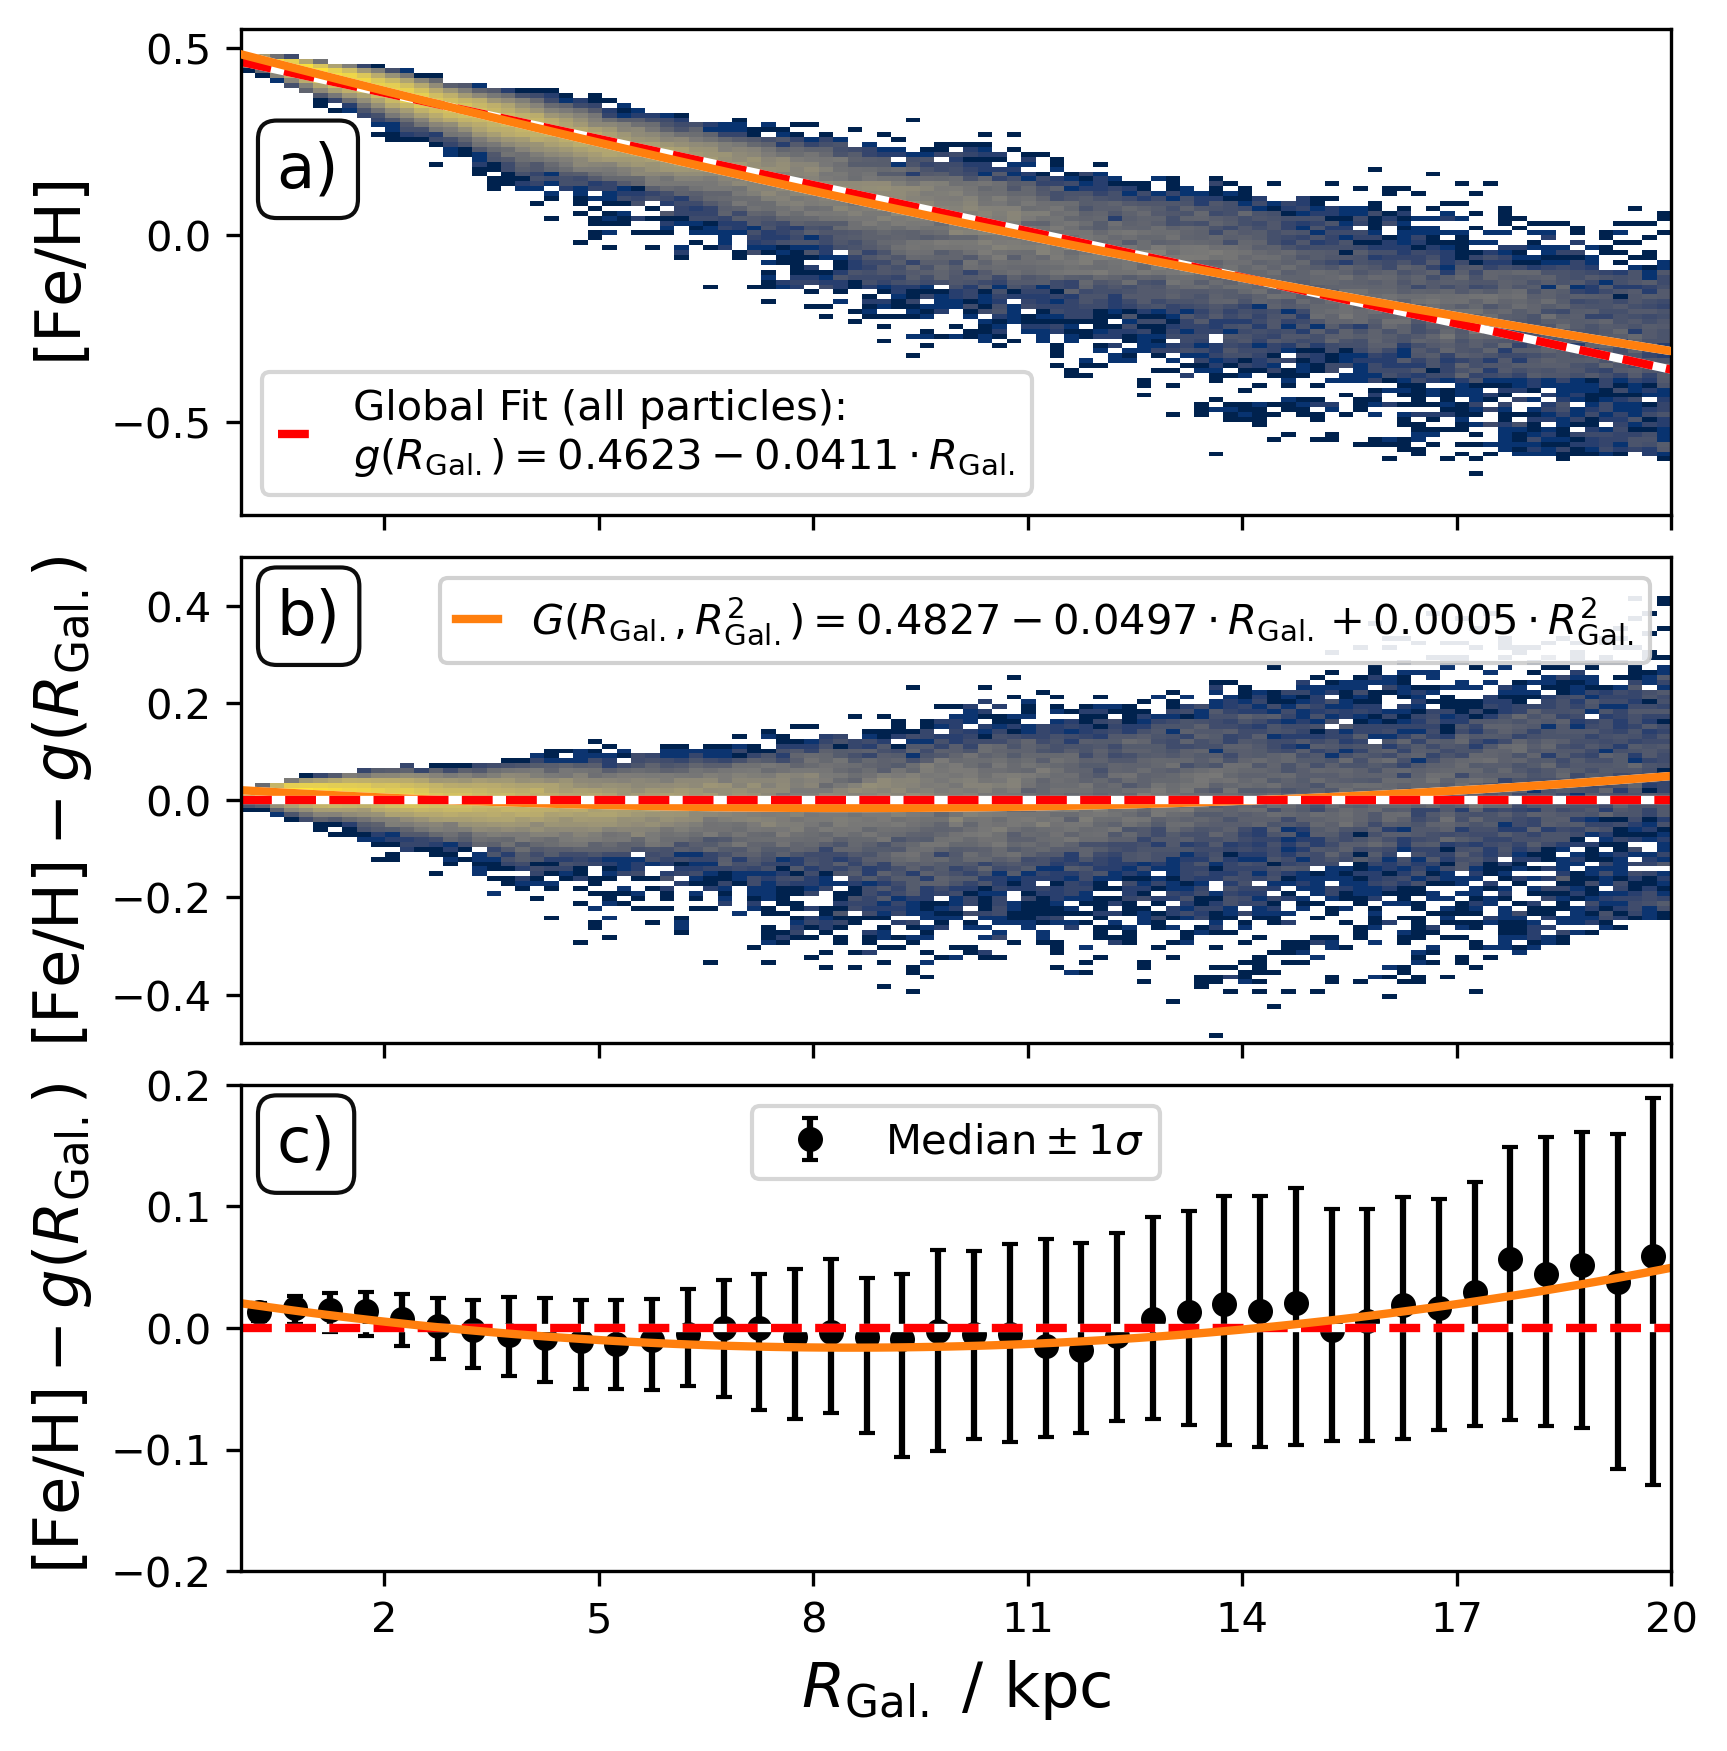
\includegraphics[width=\columnwidth]{figures/global_r_feh_fit.png}
    \caption{Global fits and deviation to the radial metallicity gradient $R-\mathrm{[Fe/H]}$. Functional forms of the linear (red) and quadratic (orange) lines are shown in the legend. Panel a) shows the underlying data of all data points as logarithmic density and the global fit to them as red dashed line. Panel b) shows the deviation of data from a linear gradient as logarithmic density plot, whereas panel c) shows the 16th and 84th percentile around the median deviation as error bars in $\Delta R_\mathrm{Gal} = 0.5\,\mathrm{kpc}$ bins.}
    \label{fig:global_r_feh_fit}
\end{figure}

We show the fit residuals in Fig.~\ref{fig:global_r_feh_fit}b as density distribution as well as in Fig.~\ref{fig:global_r_feh_fit}c as percentile distributions in radial bins of $\Delta R_\mathrm{Gal} = 0.5\,\mathrm{kpc}$. While the density distribution shows a lot of substructure, that we are investigating later in Section~\ref{sec:scatter_radial_metallicity_gradients}, we note an increase of the median residuals in Fig.~\ref{fig:global_r_feh_fit}c towards inner and outer radii, especially for $R_\mathrm{Gal.} > 17\,\mathrm{kpc}$. This suggests a non-linear, that is, quadratic component to the gradient, which we will follow up in Section~\ref{sec:non-linear_component}.

\subsection{The impact of radial coverage on linear fits}

While we have gained a useful insight into the global function, observational data will rarely cover the full extend of the stellar disk. Using smaller ranges, observational studies have found hints of piece-wise linear gradients with a break radius in them based on a limited radial coverage \citep[e.g.][]{Yong2012, Donor2020, Chen2023}.

These results are intriguing, since a quadratic function can to first order be approximated by two linear functions with a break radius. We therefore want to use this simulation to test if the radial coverage may indeed delude us into identifying broken linear gradients.

For this purpose, we are fitting and comparing linear radial metallicity gradients to subsets in galactocentric radius. We test fits across piece-wise linear radial ranges of 0.25, 0.5, 1, 2, 5, 8, 10, 15, and $20\,\mathrm{kpc}$. We show their difference with respect to a global linear fit in Fig.~\ref{fig:radial_range_impact}, with color-coding indicating the local gradient slope. In this figure, a horizontal dashed line indicates the same slope as the global fit, whereas the offset of a line from said horizontal dashed line indicates the local deviation from the global gradient intercept ($\beta$ in eq.~\ref{eq:fit_eq}). Differences in line slopes are visualising the difference in gradient slopes between the global and local fits. We see that all ranges are suggesting more or less significant deviations from a global linear fit. The innermost fit is suggesting a significantly different gradient than the outermost fit. We also note increasing slope differences towards the smallest scales, hinting at local deviations from a global pattern. We follow these up in Section~\ref{sec:scatter_radial_metallicity_gradients}, but for now focus on the larger-scale trends.

When directly comparing an inner and outer radius fit, such as between $R_\mathrm{Gal.} = 5-10\,\mathrm{kpc}$ (thick grey line in Fig.~\ref{fig:radial_range_impact}) and $R_\mathrm{Gal.} = 10-15\,\mathrm{kpc}$ (thick black line in Fig.~\ref{fig:radial_range_impact}), we note a significant change, similar to previous estimates of the Milky Way \citep[e.g.][]{Yong2012, Lemasle2008}. In our case the gradient estimate changes from $\mathrm{[Fe/H]}(R_\mathrm{Gal.}) = 0.471-0.044\cdot R_\mathrm{Gal.}$%
 to $\frac{\mathrm{d[Fe/H]}}{\mathrm{d}R_\mathrm{Gal.}} = 0.383-0.035\cdot R_\mathrm{Gal.}$%
. When looking at linear gradient fits across radial coverage of $\Delta R_\mathrm{Gal.} = 5-15\,\mathrm{kpc}$ in Fig.~\ref{fig:radial_range_impact}, the gradient was steeper (bluer color) for smaller radii and flatter (redder) for larger radii.

While such effects have been seen before for the Milky Way, previous studies have mostly suggested to fit piece-wise linear gradients with a break radius \citep[e.g.][]{Andrievsky2002, Yong2012, Boeche2013, Hayden2014, Anders2017, Donor2020}. Our results from Fig.~\ref{fig:radial_range_impact} suggest, however, not a gradient with a break radius, but rather a smoothly evolving flattening gradient, in better agreement with a quadratic function rather than two linear ones. In this section, we are therefore trying to expand the gradient function by a higher order, that is, a second order one.

\begin{figure}
    \centering
    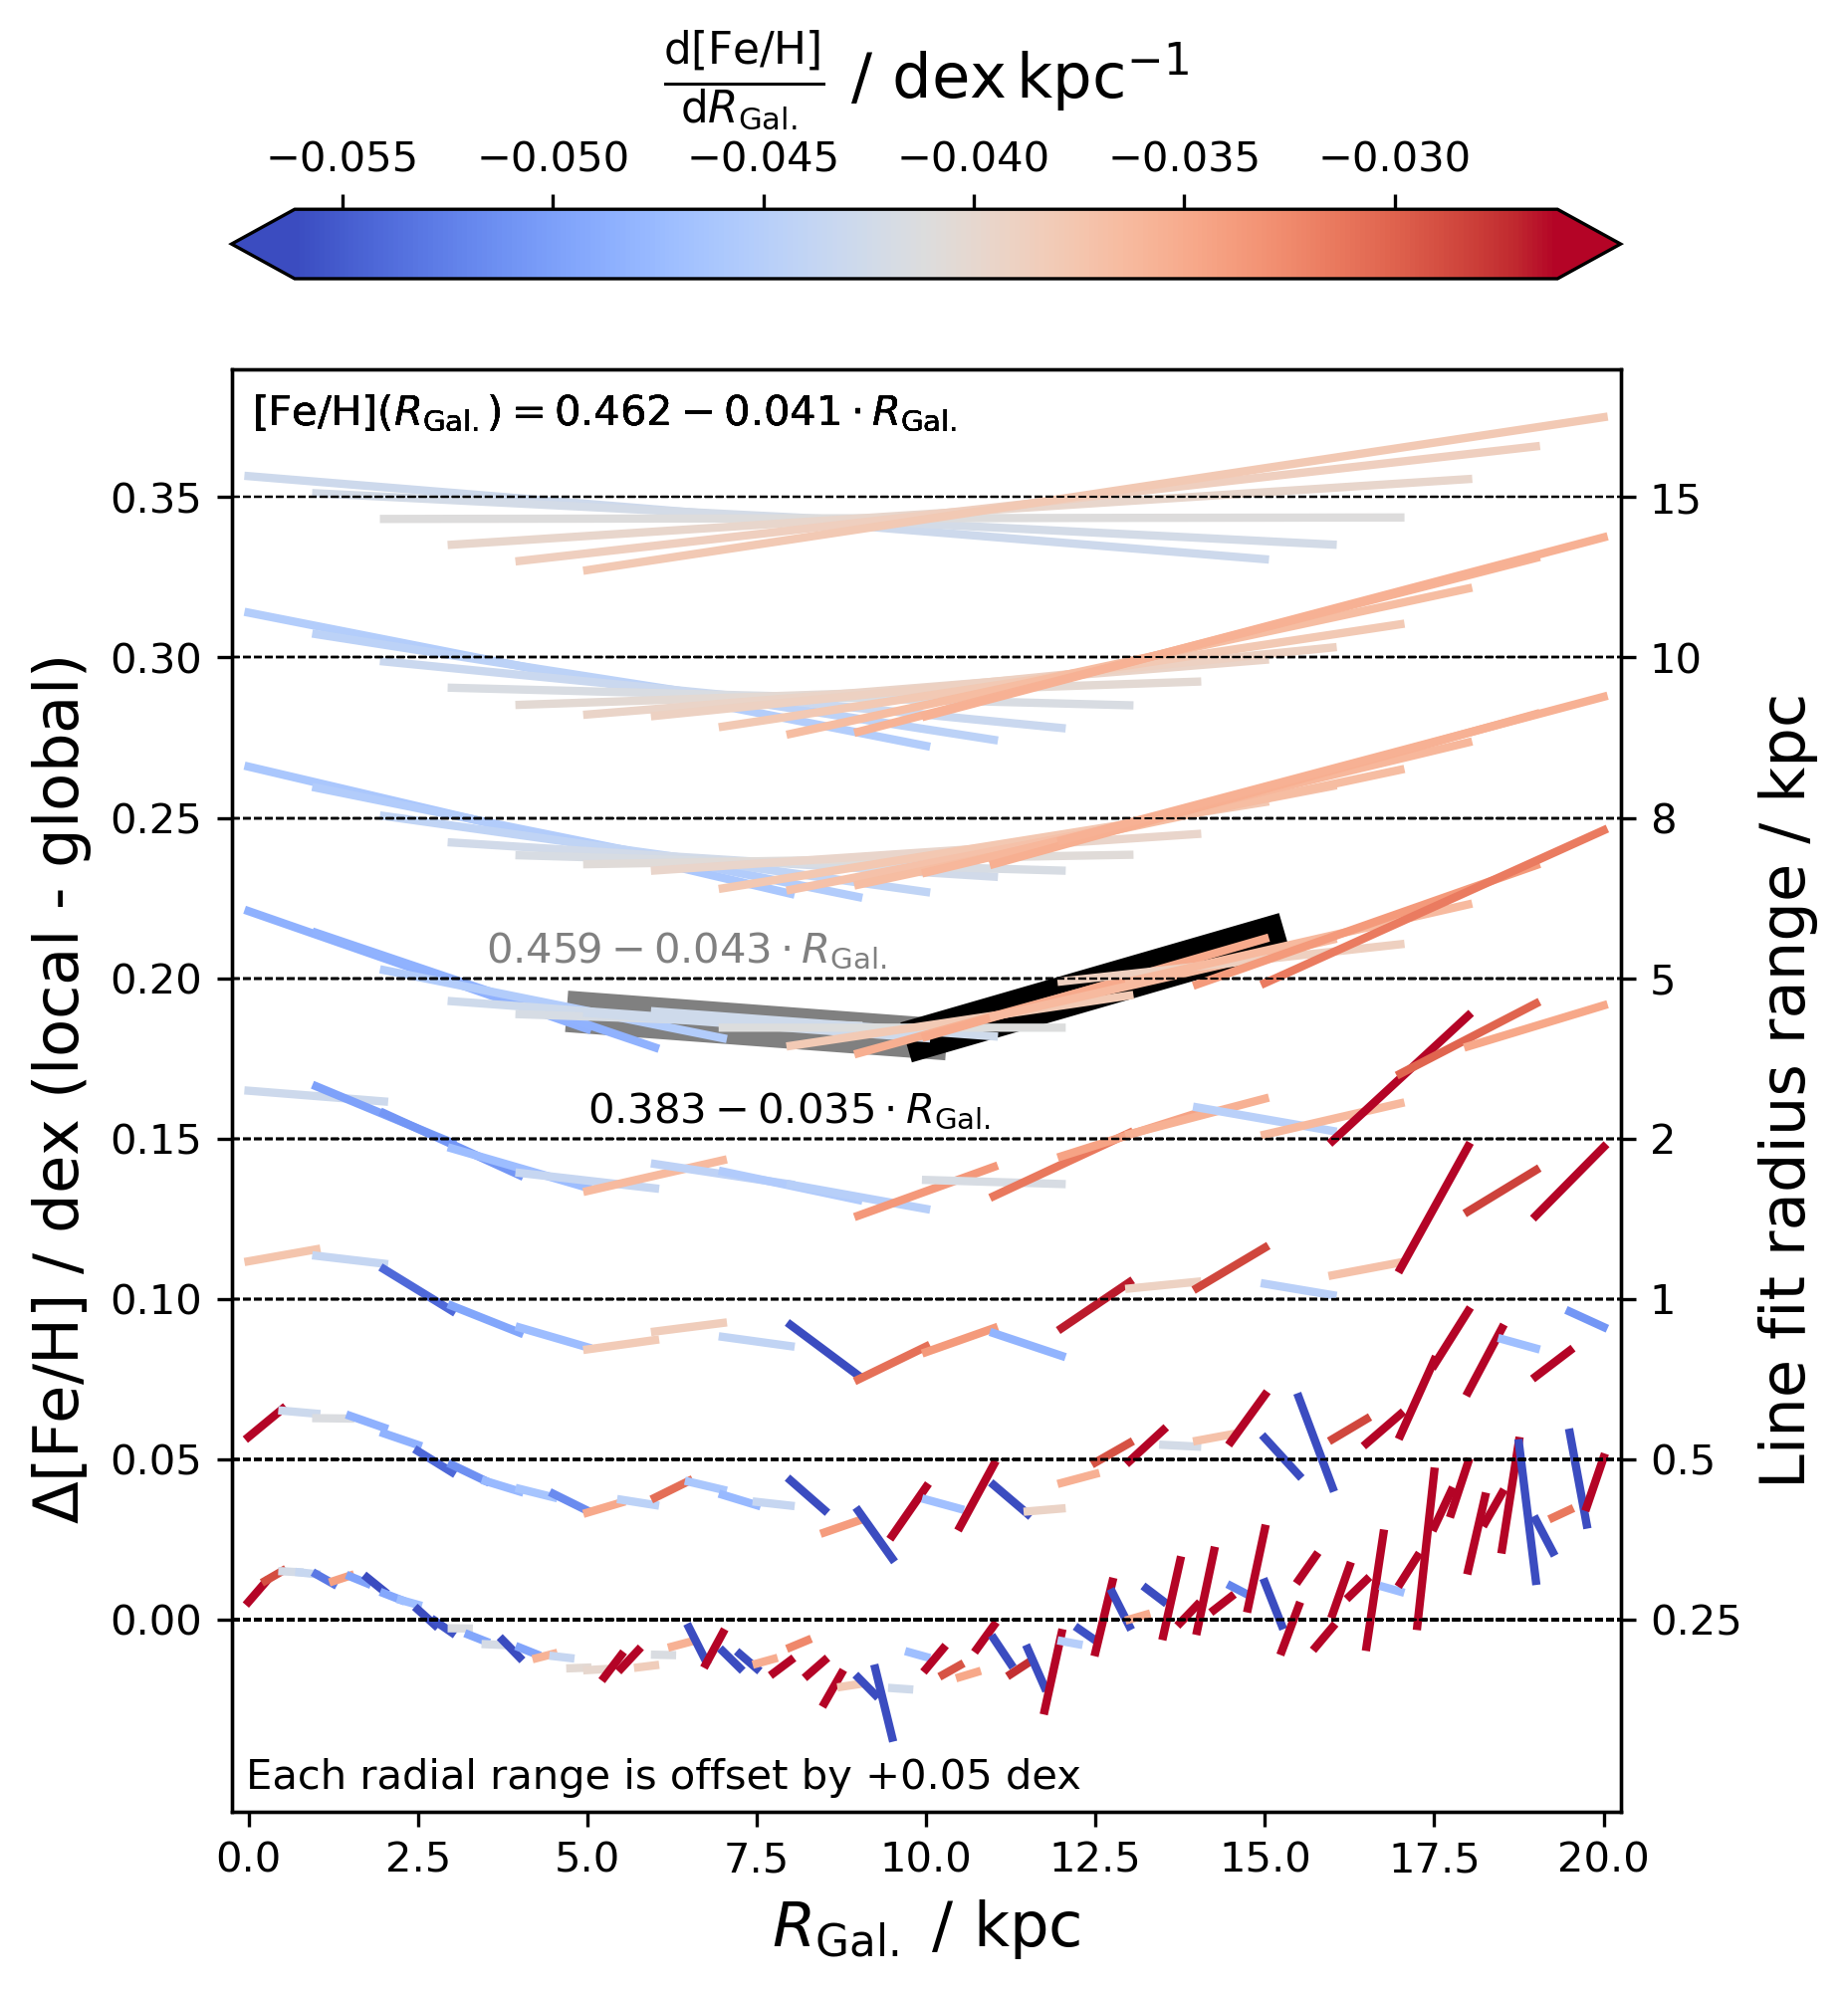
\includegraphics[width=\columnwidth]{figures/radial_range_impact.png}
    \caption{Impact of different coverage in galactocentric radius when fitting a linear radial metallicity gradient to young stars. Each horizontal segment is using a different running radial fitting range between 0.25 and $15\,\mathrm{kpc}$ as outlined on the right. For better contrast, the global linear fit is subtracted from the local gradient estimates and each line is colored by the gradient slope with a color scale centered around the global fit slope. Additionally, the slope of each line segment highlights the difference between global and local slope. This means, if the local fit exactly matches the global fit, we display it as a flat line (zero slope difference) on top of the gray dashed line (zero offset deviation) and give it a gray color signaling the same gradient value as the global fit.}
    \label{fig:radial_range_impact}
\end{figure}

\subsection{Higher-order gradients} \label{sec:non-linear_component}

A quadratic fit (see orange lines in Fig.~\ref{fig:global_r_feh_fit}) results in a slightly steeper linear component of the gradient (from $-0.0411$ to $-0.0497\,\mathrm{dex\,kpc^{-1}}$), which is counteracted by the quadratic flattening term of $+0.0005\,\mathrm{dex\,kpc^{-2}}$. The latter leads to an effective flattening of $-0.172 + 0.200 = 0.028\,\mathrm{dex}$ (linear vs. quadratic terms) at $R_\mathrm{Gal.} = 20\,\mathrm{dex}$. While seemingly only a nuisance correction across the large extend of [Fe/H] and $R_\mathrm{Gal.}$, this quadratic function is evidently superior to the linear fit. This can be best appreciated in Fig.~\ref{fig:global_r_feh_fit}c, where the orange line is tracing the median residuals from the linear function much better across all the radii.

\begin{figure}
    \centering
    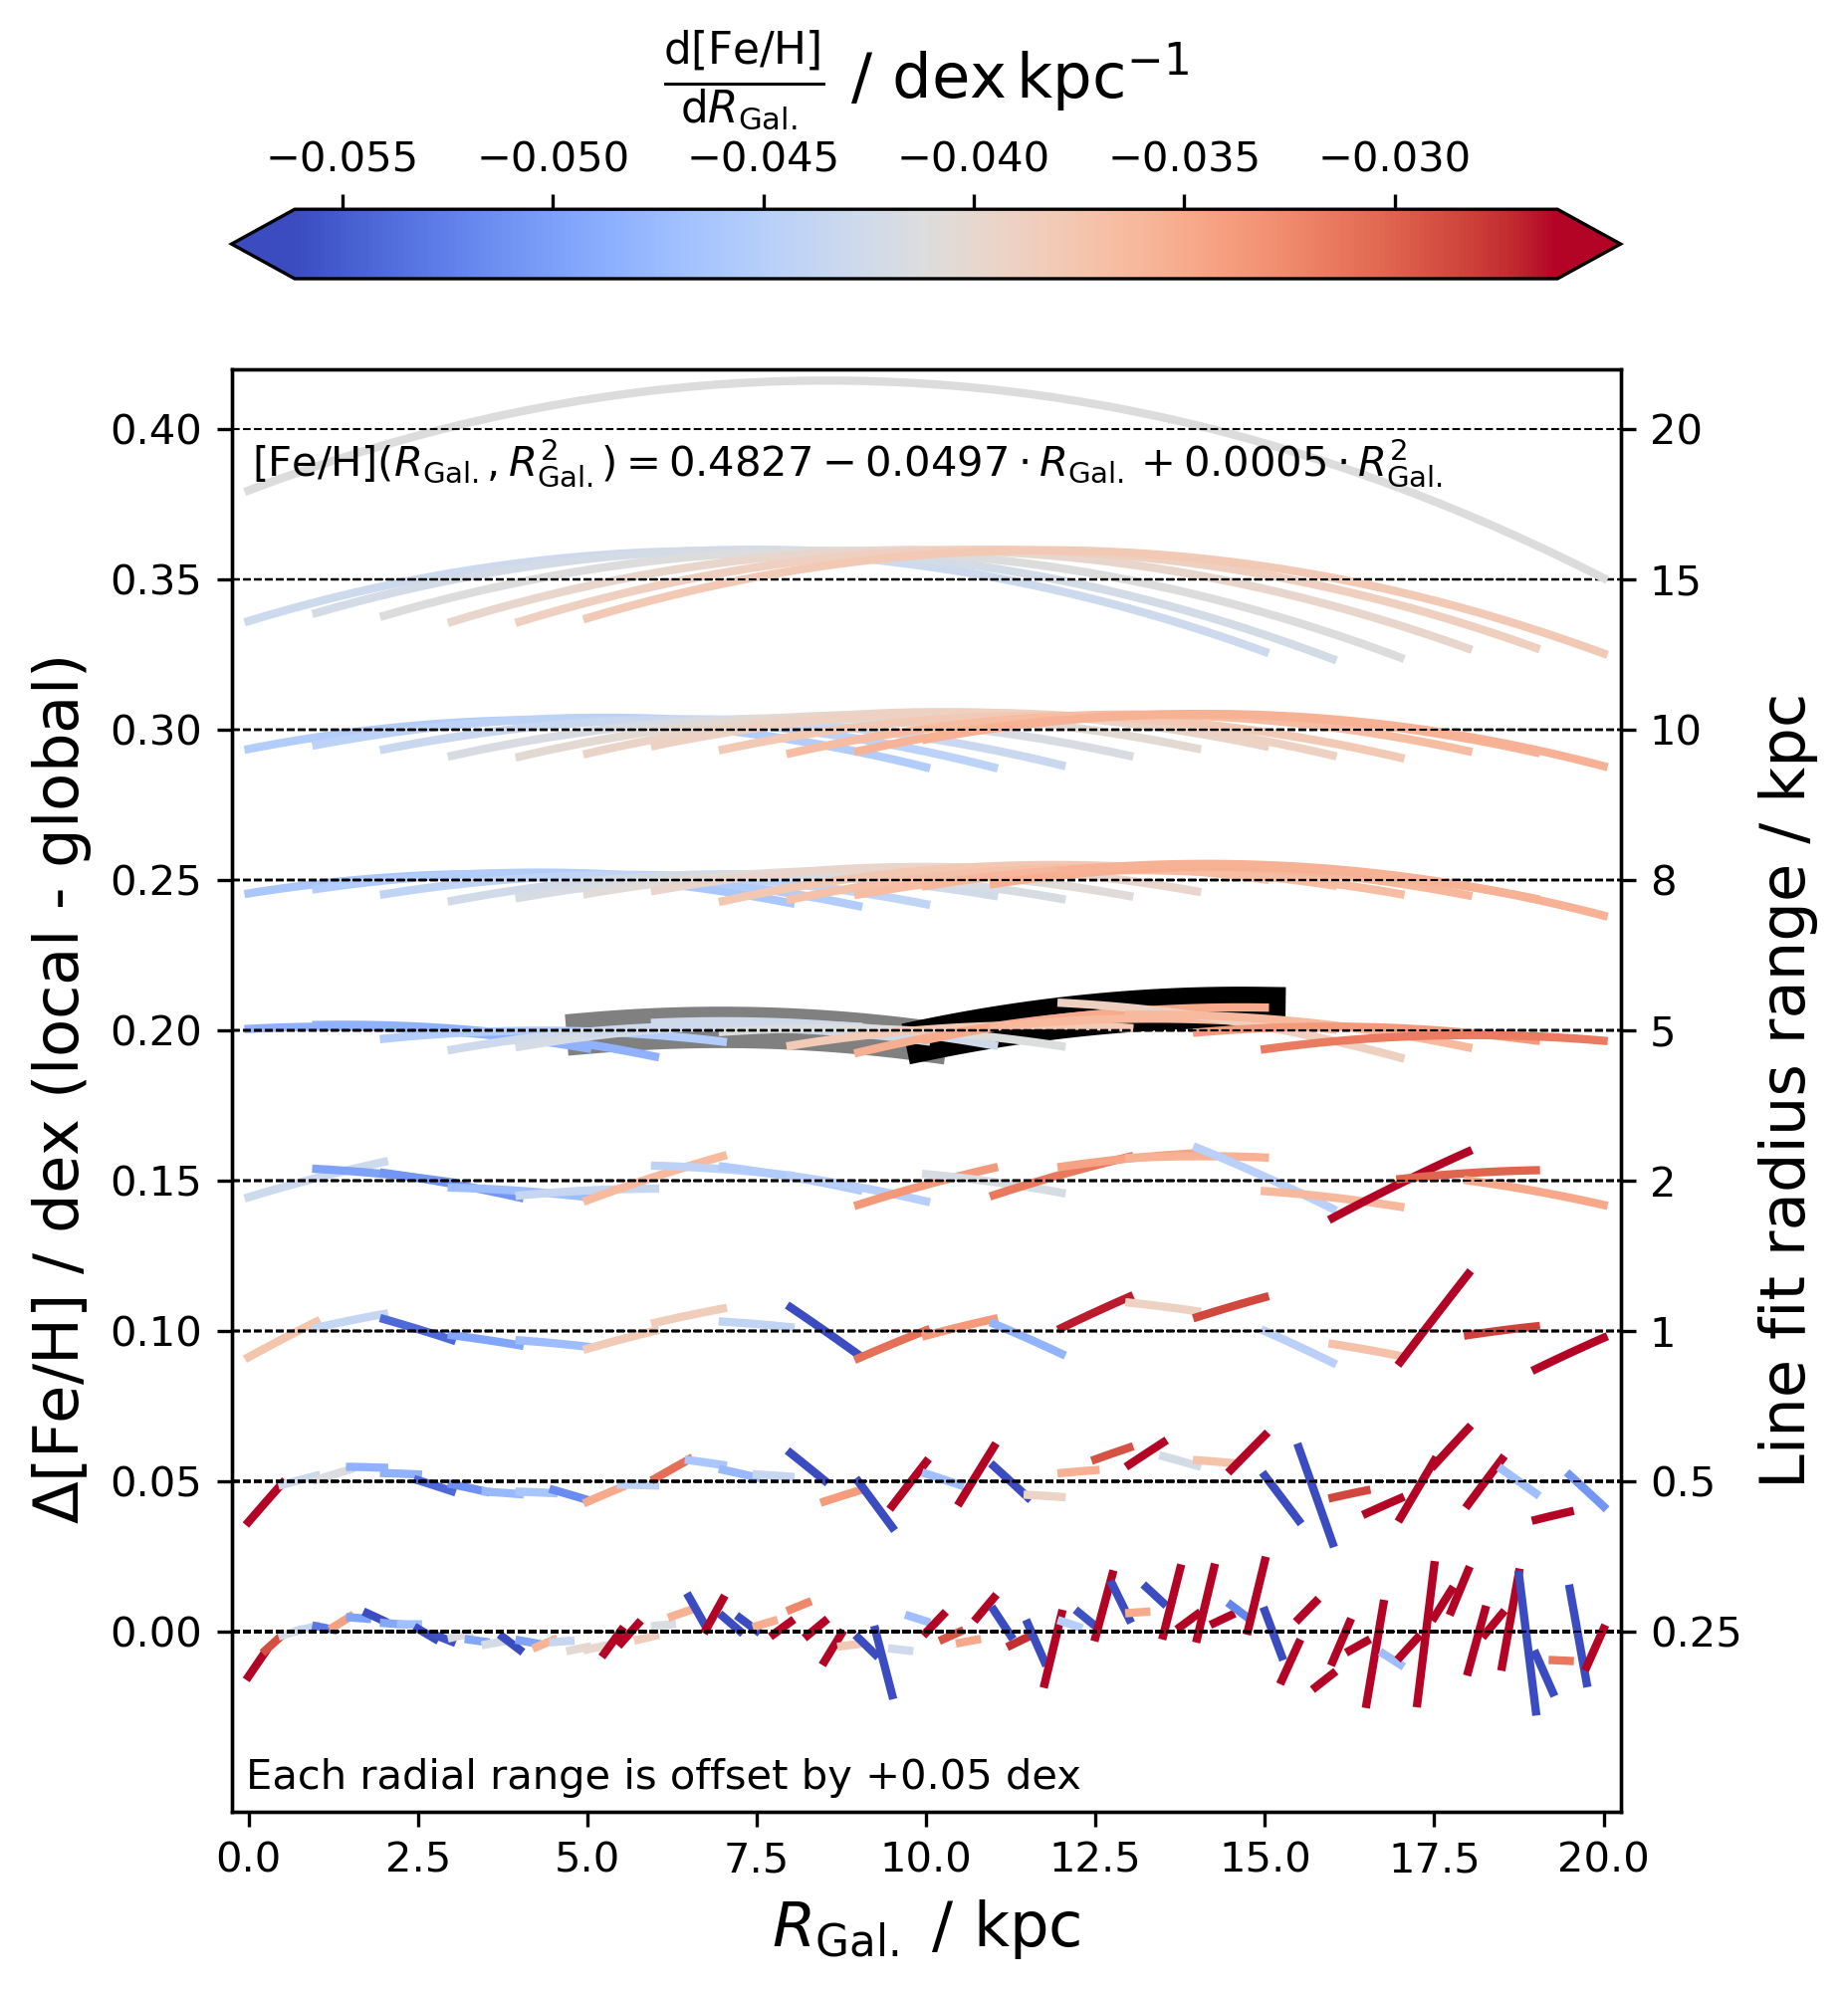
\includegraphics[width=\columnwidth]{figures/radial_range_impact_quadratic.png}
    \caption{Same as Fig.~\ref{fig:radial_range_impact}, but comparing local deviations to a quadratic global fit. Overall deviations have decreased most notably for innermost and outermost radii.}
    \label{fig:radial_range_impact_quadratic}
\end{figure}

\SB{Analyse here both quadratic and piecewise linear fit and how to decide which one works better with RSS, AIC, and BIC with number of free parameters $k$ to fit the $n$ datapoints:}

Having fitted three different models, will use a combination of parameters to judge which model fits better. Firstly, we are computing the residual sum of squares ($RSS$) as 
\begin{equation} \label{eq:rss}
    RSS = \sum_i^n \left( \mathrm{[Fe/H]} - g(R_\mathrm{Gal.}) \right)^2.
\end{equation}


\begin{table*}
\caption{
Fit Evaluation of linear, quadratic, and piecewise linear fits.
Extra parameters are quadratic term and break radius for the quadratic and piecewise fit.
RSS stands for Residual Sum of Squares (Eq.~\ref{eq:rss}).
AIC stands for Akaike Information Criterion and BIC stands for Bayesian Information Criterion (see Eq.~\ref{eq:aic_bic}).
}
\label{tab:global_fit_results_comparison}
\begin{tabularx}{\textwidth}{lCCCccc}
\hline
Function & Intercept ($a_0 \pm \sigma_{a_0}$) & Slope ($a_1 \pm \sigma_{a_1}$) & Extra Parameter & RSS & AIC & BIC \\
\hline
Linear & $0.46849 \pm 0.00159$  & $-0.04169 \pm 0.00035$ & -- & 87.6 & -118050  & -118030 \\ 
Quadratic & $0.48031 \pm 0.00055$  & $-0.04864 \pm 0.00018$ & $0.00045 \pm 0.00001$ & 82.7 & -120150  & -120120 \\ 
Piecewise & $-0.04477 \pm 0.00010$ & $0.47473 \pm 0.00047$ & -- & 82.9 & -120090  & -120050 \\ 
 & -- & $-0.03562 \pm 0.00014$ & $9.3$ & & & \\ 
\hline
Linear (bins)& $0.46849 \pm 0.00567$  & $-0.04169 \pm 0.00127$ & -- & 0.0147 & -200  & -200 \\ 
Quadratic (bins) & $0.47327 \pm 0.00674$  & $-0.04611 \pm 0.00359$ & $0.00031 \pm 0.00024$ & 0.0033 & -260  & -250 \\ 
Piecewise (bins) & $-0.04398 \pm 0.00207$ & $0.47190 \pm 0.00617$ & -- & 0.0026 & -260  & -260 \\ 
 & -- & $-0.03547 \pm 0.00461$ & $10.0$ & & & \\ 
\hline
\end{tabularx}
\end{table*}


We see from Table~\ref{tab:global_fit_results_comparison} that this value is smallest (although only by a small margin) for the quadratic function. When assuming $\sigma^2 = RSS / n$, we can then define a logarithmic likelihood
% in statsmodels:
% https://www.statsmodels.org/dev/_modules/statsmodels/regression/linear_model.html#OLS.loglike
% nobs2 = self.nobs / 2.0
% nobs = float(self.nobs)
% resid = self.endog - np.dot(self.exog, params)
% ssr = np.sum(resid**2)
% llf = -nobs2*np.log(2*np.pi) - nobs2*np.log(ssr / nobs) - nobs2
\begin{equation}
    \ln L = - \frac{n}{2} \ln (2 \pi) - \frac{n}{2} \ln \frac{RSS}{n} - \frac{n}{2}
\end{equation}
for our $n$ data points. For $k$ free parameters, we can then calculate the Akaike Information Criterion (AIC) and the Bayesian Information Criterion (BIC) as
\begin{equation} \label{eq:aic_bic}
    AIC = 2 k  - 2 \ln L \qquad BIC = k \ln n - 2 \ln L.
\end{equation}
Again, the quadratic function performs slightly better than the linear or piecewise linear functions (see Table~\ref{tab:global_fit_results_comparison}).

\SB{CONTINUE STATEMENT HERE WHAT THAT MEANS. Should we also still try MCMC? In any case, we should try to fit in bins.}

When reproducing the local deviations from the linear global fit (Fig.~\ref{fig:radial_range_impact}) with a quadratic global fit (Fig.~\ref{fig:radial_range_impact_quadratic}), we see that the deviations of the local fits no longer have significant offsets with respect to the horizontal lines, while still showing the increasing slope differences at the local levels (especially on scales below $1\,\mathrm{kpc}$). 

%%%%%%%%%%%%%%%%%%%%%%%%%%%%%%%%%%%%%%%%%%%%%%%%%%
\section{Scatter and local deviations from the gradient}
\label{sec:scatter_radial_metallicity_gradients}

Now that we are sufficiently satisfied that our flattening gradient function reproduces the overall shape of the radial metallicity gradient, we are concerned with both the scatter and local slope deviations across the galactocentric radii.

When investigating the change of scatter from the innermost radii to the outermost (see Fig.~\ref{fig:global_r_feh_fit}c), we see a steady increase in $1-\sigma$ spread. This spread increases from
\begin{description}
    \item $\sigma \mathrm{[Fe/H]} = 0.01\,\mathrm{dex}$%
 at $R_\mathrm{Gal.} = 0.25 \pm 0.25\,\mathrm{kpc}$ to
    \item $\sigma \mathrm{[Fe/H]} = 0.06\,\mathrm{dex}$%
 at $R_\mathrm{Gal.} = 8.25 \pm 0.25\,\mathrm{kpc}$ and finally reaches 
     \item $\sigma \mathrm{[Fe/H]} = 0.10\,\mathrm{dex}$%
 at $R_\mathrm{Gal.} = 19.75 \pm 0.25\,\mathrm{kpc}$, the largest $R_\mathrm{Gal.}$.
\end{description}

When reminding ourselves of the observed significant spread in metallicities of young open cluster at the solar radius beyond observational uncertainty \citep[e.g.][]{Donor2020, Spina2021} and our selection of only young ($<$\nihaoAGEmax) stars from the simulation, a strong impact of this scatter by radial migration should be excluded. At this point, we can imagine that this chemical diversity might be caused by less well mixed gas or non-radial effects (such as vertical or azimuthal ones), which we investigate subsequently.

\begin{figure}
    \centering
    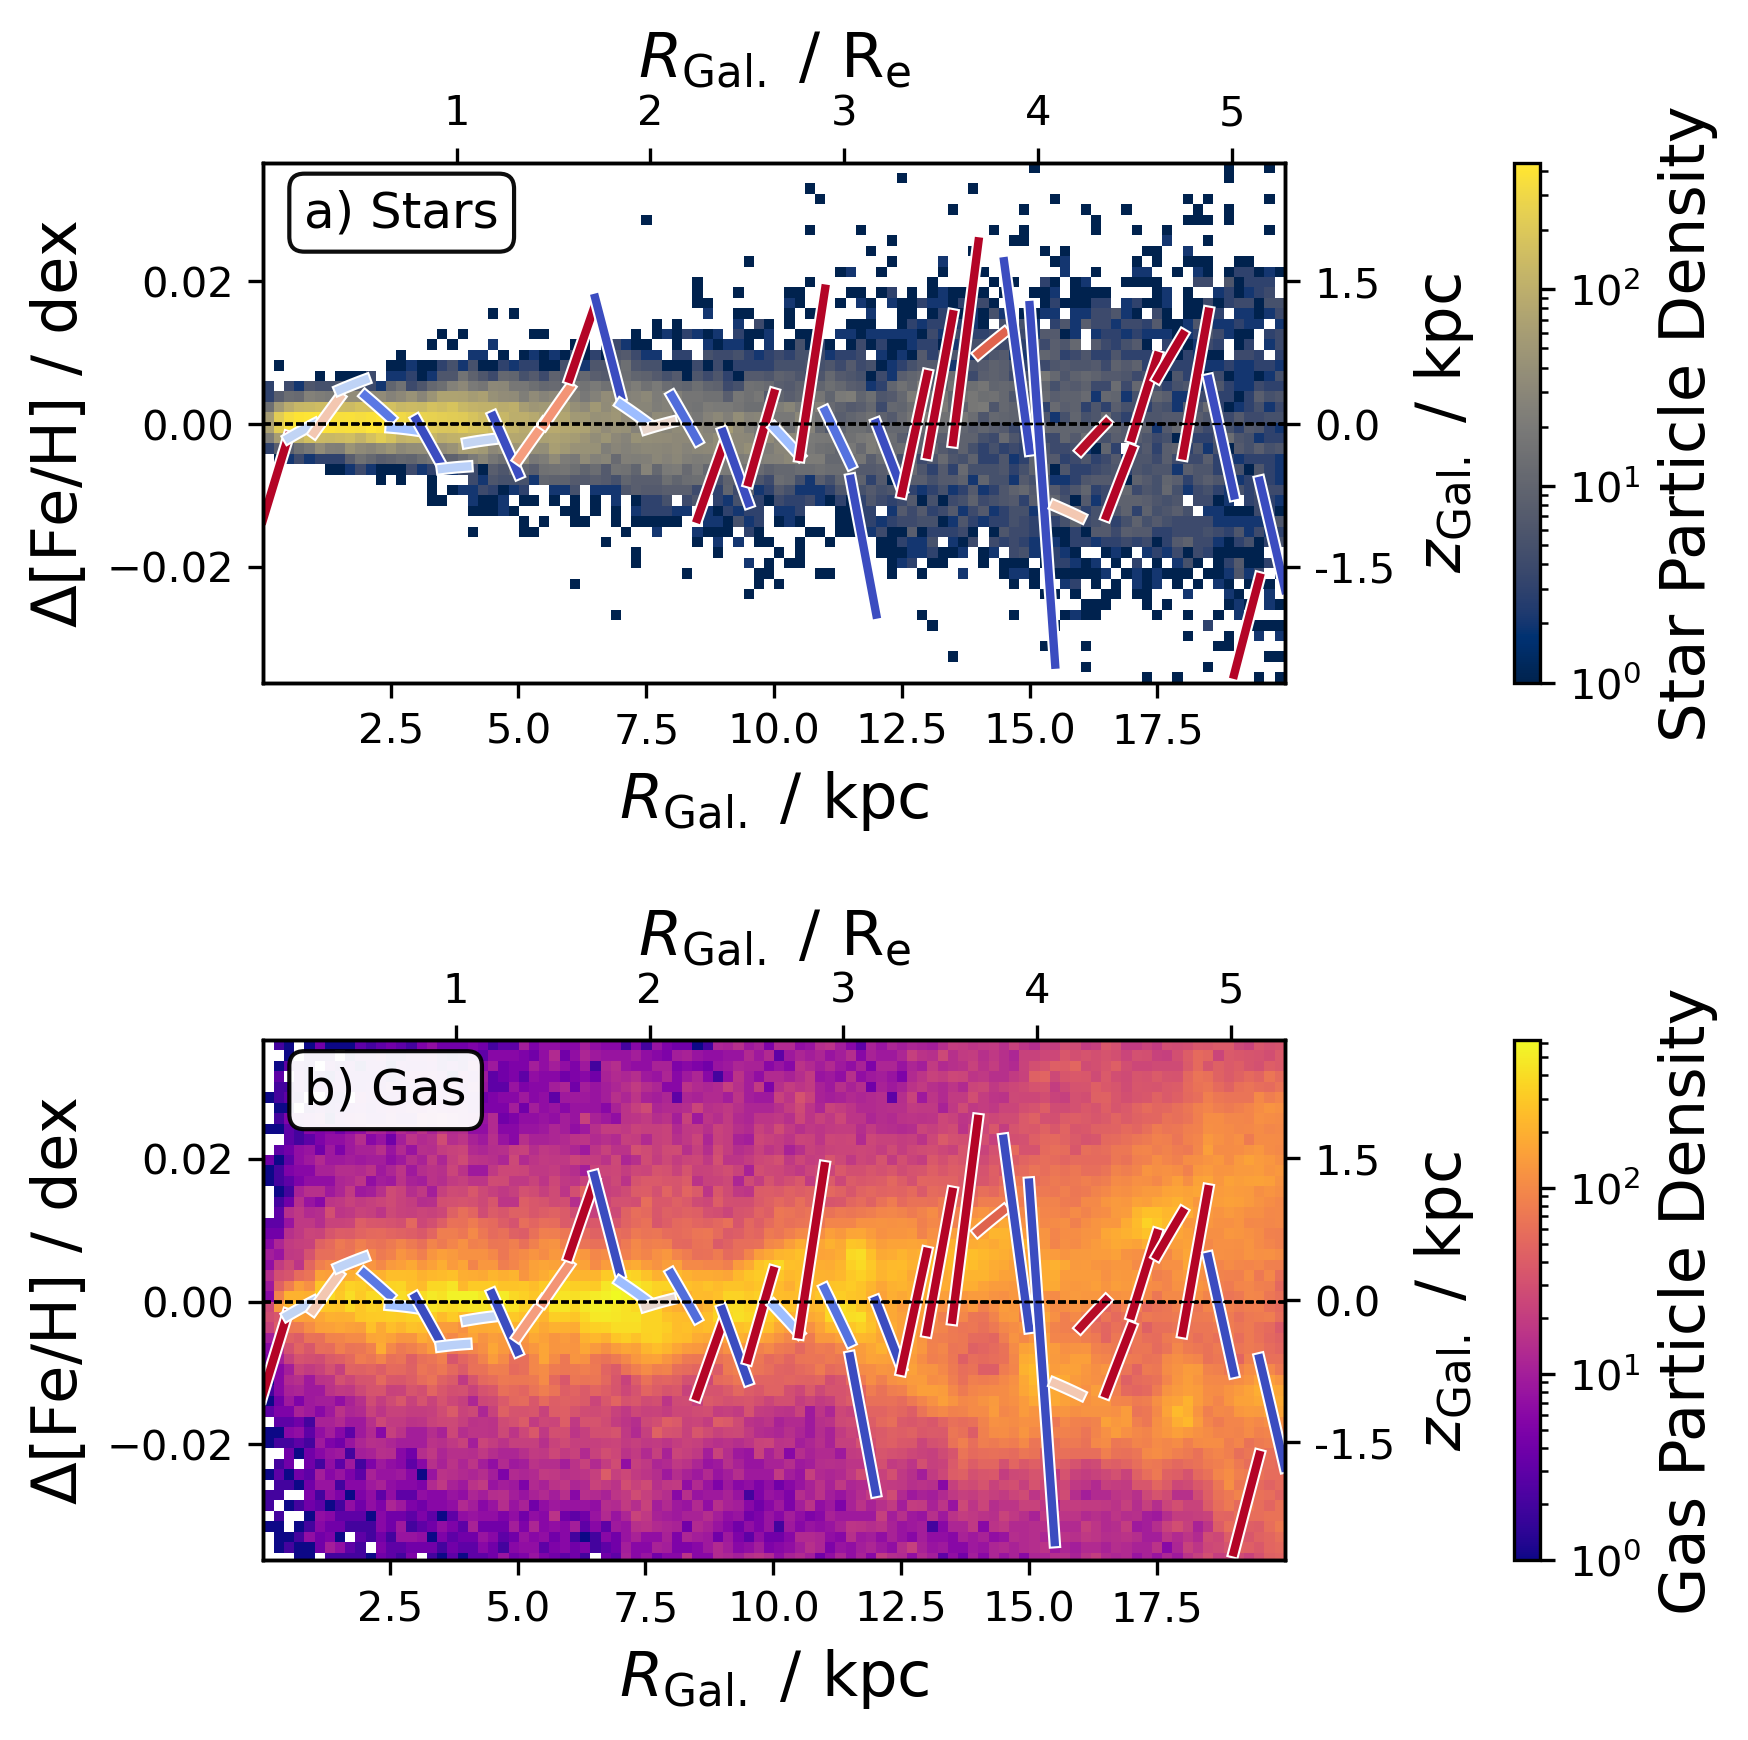
\includegraphics[width=\columnwidth]{figures/overlap_local_variation_gas.png}
    \caption{Local gradient deviations from second lowest row of Fig.~\ref{fig:radial_range_impact_quadratic} for radial gradients in $0.5\,\mathrm{kpc}$ steps overlapped on top of the logarithmic density distribution in $R-z$ for $\vert z \vert < 3\,\mathrm{kpc}$ of gas (panel a) and stars (panel b).}
    \label{fig:overlap_local_variation_gas}
\end{figure}

\subsection{Gradient deviations with vertical position}
\label{sec:coherence_vertical_radial_metallicity_gradients}

In this section, we are now looking into deviations with respect to the vertical dimension. In Fig.~\ref{fig:overlap_local_variation_gas} we are showing the previously identified gradient deviations (lines following the left axis label) on top of the vertical density distribution ($R-z$) of gas (Fig.~\ref{fig:overlap_local_variation_gas}a) and young stars (Fig.~\ref{fig:overlap_local_variation_gas}b) between $-3 < z < 3\,\mathrm{kpc}$. While the quickly decreasing amount of young stars (Fig.~\ref{fig:overlap_local_variation_gas}b) at outer radii does not show substructure in the density plots for reasonable bin sizes, we see more substructure for the gaseous component in Fig.~\ref{fig:overlap_local_variation_gas}a). In particular, we see rather minor deviations at small radii (where most stars and gas are close to the plane). At increasing radii, we notice an increase in both the vertical distribution of stars, as well as increasing local gradient deviations. In particular, we note a significant deviation of the slope around $R_\mathrm{Gal.} \sim 15\,\mathrm{kpc}$, where the gradient deviation line is steep and blue (indicating a much steeper gradient at this radius), and we notice a significant overdensity of gas around $z \sim 1\,\mathrm{kpc}$.

While such an edge-on view of the galaxy may indeed be the only observable one for extra-galactic targets, for example of the GECKOS survey of edge-on galaxies \citep{GECKOS2023}, we have the luxury of being able to analyse the azimuthal direction of our simulated galaxy, too. This seems especially important, as we have seen a significant warping of the gaseous and stellar disk of our simulated galaxy (see Figs.~\ref{fig:stars_and_gas_overview}b and \ref{fig:stars_and_gas_overview}e). While the warp of the stellar disk in Fig.~\ref{fig:stars_and_gas_overview}b is not as clear, we confirm that both the gas disk and the youngest stars below \nihaoAGEmax\ are tracing each other across the simulation in both galactocentric radius $R_\mathrm{Gal.}$ and height $z_\mathrm{Gal.}$ for different sectors in azimuthal direction.

\begin{figure*}
    \centering
    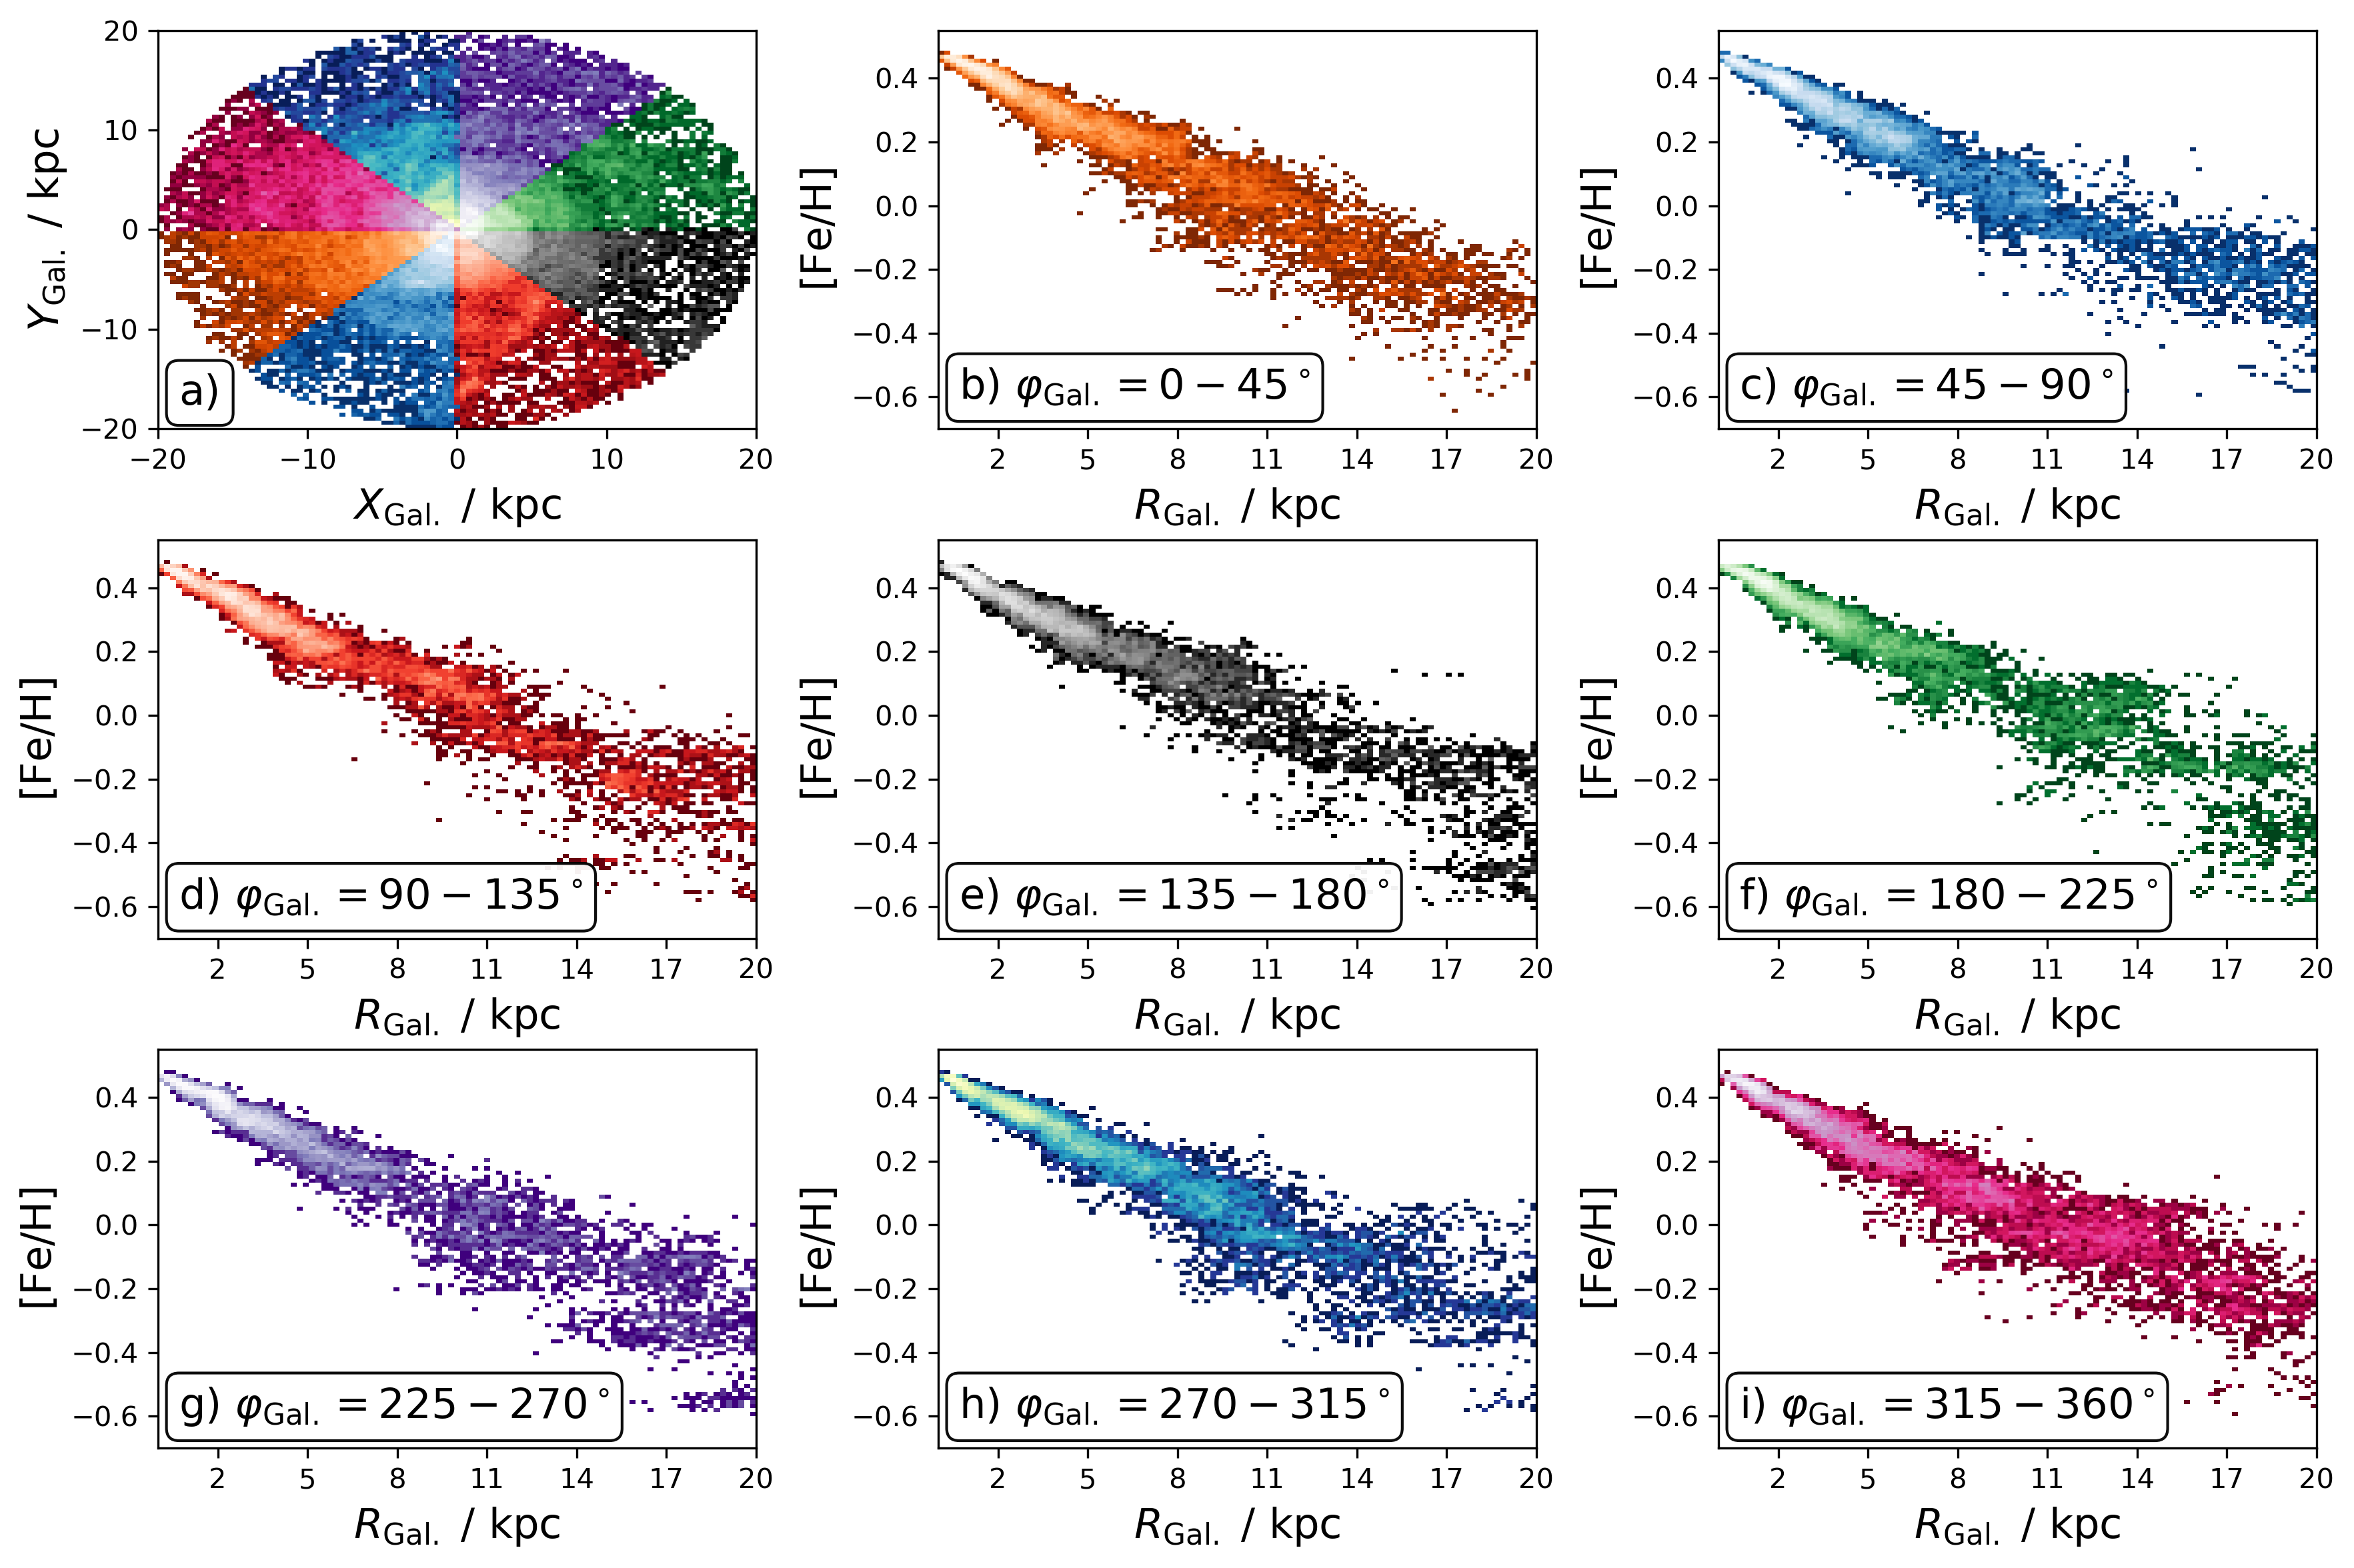
\includegraphics[width=0.875\textwidth]{figures/radial_metallicity_gradients_mw_in_angles.png}
    \caption{Stellar density variation across 8 different sectors (with color-code visualised in panel a) of the radial metallicity gradient $R-\mathrm{[Fe/H]}$ across 8 different azimuth ranges (panels b-i). A rotating lighthouse-like GIF animation of the median age and median density of the $R-\mathrm{[Fe/H]}$-relation across different azimuths is freely available on a \href{https://github.com/svenbuder/nihao_radial_metallicity_gradients/blob/main/figures/xyz_rfeh.gif}{repository}.}
    \label{fig:radial_metallicity_gradients_mw_in_angles}
\end{figure*}

\begin{figure*}
    \centering
    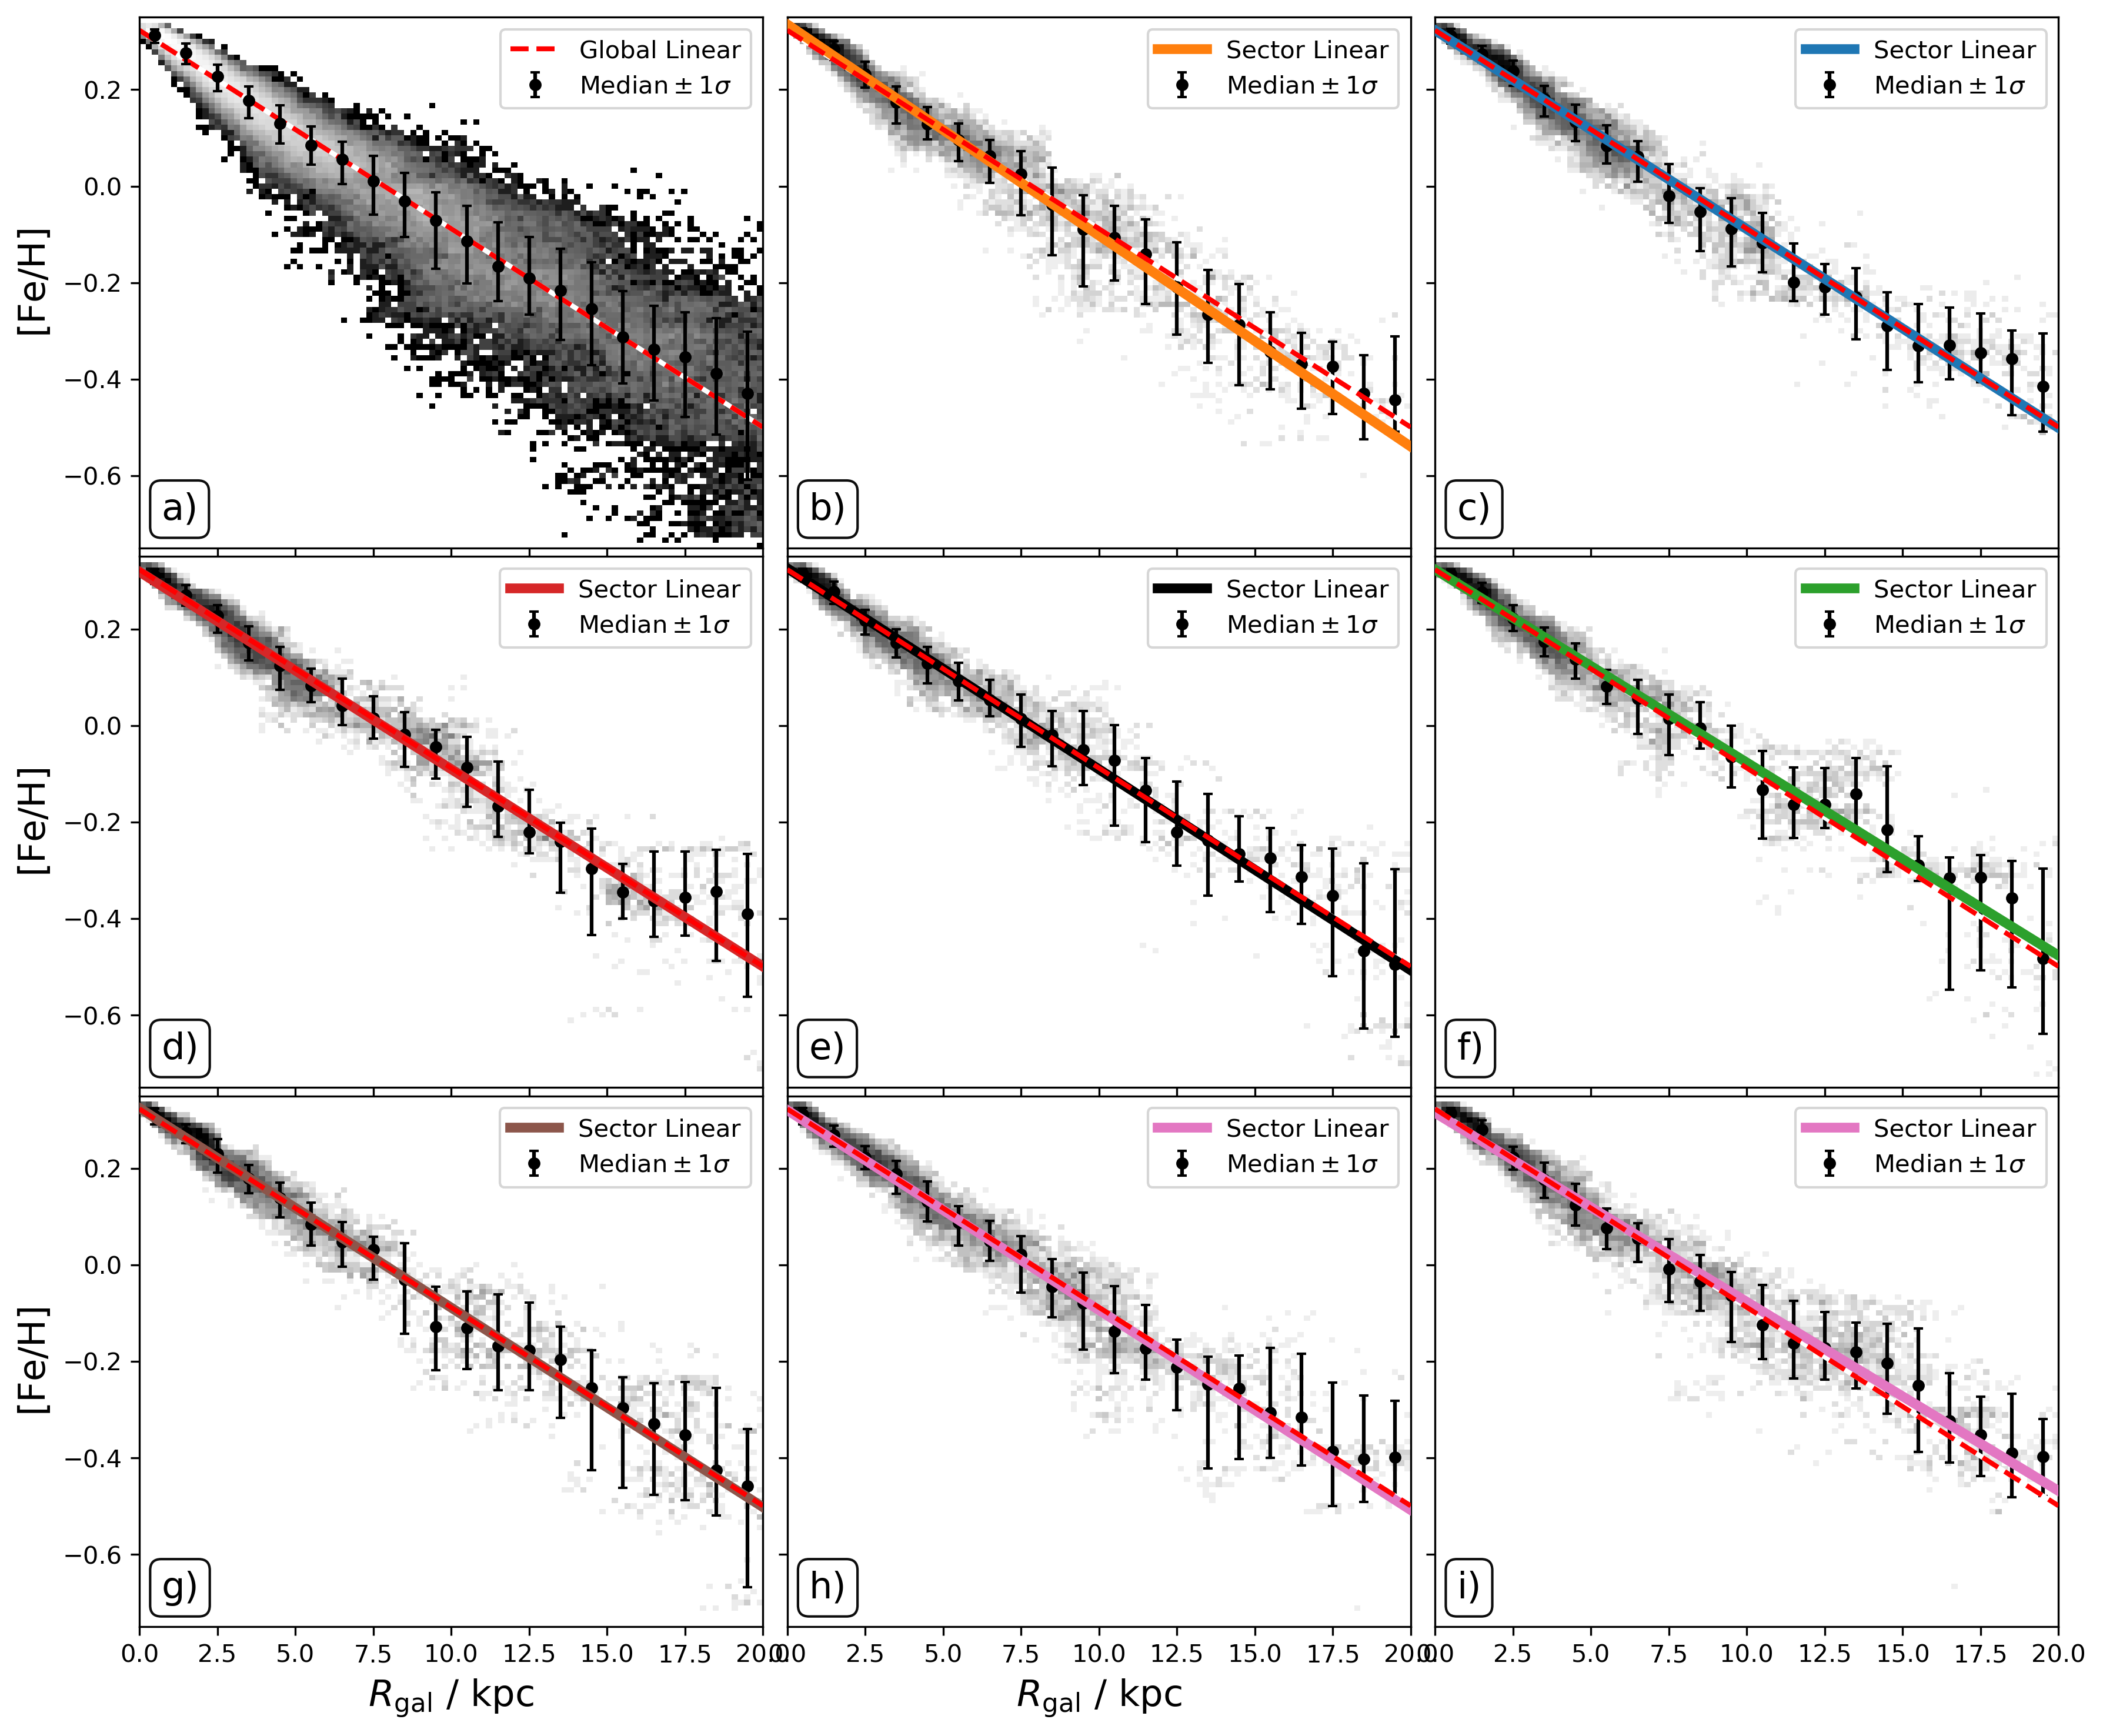
\includegraphics[width=0.875\textwidth]{figures/linear_radial_metallicity_gradients_mw_in_angles.png}
    \caption{Stellar density variation of the radial metallicity gradient $R-\mathrm{[Fe/H]}$ across full stellar disk (panel a) and 8 different sectors (same panel order as for Fig.~\ref{fig:radial_metallicity_gradients_mw_in_angles}). Linear radial metallicity gradients have been fit globally (red dashed line) and for each sector with colors following the same color code as in Fig.~\ref{fig:radial_metallicity_gradients_mw_in_angles}.}    \label{fig:linear_radial_metallicity_gradients_mw_in_angles}
\end{figure*}

\subsection{Gradient deviations with azimuthal position}
\label{sec:coherence_azimuth_radial_metallicity_gradients}

To analyse the deviations from a global gradient across different azimuthal viewing angles, we divide the galaxy into 8 sectors with $\Delta \varpi_\mathrm{Gal.} = 45\,\mathrm{deg}$ (see Fig.~\ref{fig:radial_metallicity_gradients_mw_in_angles}a). This allows us to study the positions around the upturn and downturn of the galactic warp with the median azimuth of young star particles below and above the plane being $\varphi_\mathrm{Gal.} \sim 183\,\mathrm{deg}$ and $\varphi_\mathrm{Gal.} \sim 4\,\mathrm{deg}$, respectively (see Fig.~\ref{fig:stars_and_gas_overview}e).

\SB{CONTINUE}

\begin{itemize}
    \item Density variation of the radial metallicity gradient $R-\mathrm{[Fe/H]}$ across 8 different sectors in Fig.~\ref{fig:radial_metallicity_gradients_mw_in_angles}
    \item Deviation from global radial metallicity gradient across 8 different sectors in Fig.~\ref{fig:linear_radial_metallicity_gradients_mw_in_angles}
    \item Fig.~\ref{fig:linear_radial_metallicity_gradients_mw_in_angles}f shows impressively, that if you look at a rather narrow range of $R_\mathrm{gal}$, such as $7 < R_\mathrm{gal} < 13\,\mathrm{kpc}$, the radial metallicity gradient could actually look like it is damping towards larger radii. Actually one can see this effect even better in Fig.~\ref{fig:radial_metallicity_gradients_mw_in_angles}b,d,e,f,h and i! Is this possibly what is happening in local studies of our galaxy, where many researchers are actually fitting 2 linear gradients with a break radius?
    \item Fig.~\ref{fig:tracing_fe_h_young_stars_in_angles}
    \item Fig.~\ref{fig:tracing_fe_h_residuals_young_stars_in_angles}
    \item Idea: Compute gradient over a radius R and then plot this one in color in the xy direction (like hogg/eilers). Maybe 2kpc is the best radius to do that? Can also try 5kpc.
\end{itemize}


\subsection{Coherence of the gradient with age}
\label{sec:coherence_age_radial_metallicity_gradients}

\begin{itemize}
    \item Fig.~\ref{fig:quadratic_fit_across_maximum_ages}: Test how much the radial metallicity gradient flattens/steepens if we consider only younger or also older stars than our current cut-off.
    \item Do the same as Fig.~\ref{fig:radial_metallicity_gradients_mw_in_angles}, but with bins colored by median age: Fig.~\ref{fig:radial_metallicity_gradients_mw_in_angles_age}
    \item We track the scatter across age in Fig.~\ref{fig:scatter_with_increasing_age}.
    \item The maximum scatter in radius bins varies between $0.073\,\mathrm{dex}$ and $0.195\,\mathrm{dex}$ across the $0..0.1..1.0\,\mathrm{Gyr}$ bins.%

    \item Note the diagonal streaks in each of the small age bins (half a dynamic timescale) -> Could this be related to the spiral arms triggering star formation? How could we further trace this? color this by age or $\varphi_\mathrm{Gal.}$? These are the same features that are popping up in the GIF: same age, same [Fe/H], but different azimuth and slightly different radius (thus deviation from linear fit).
    \item Test gradient for different ages above 1 Gyr? Maybe not necessary. We see that in Fig.~\ref{fig:scatter_with_increasing_age}k and especially \ref{fig:scatter_with_increasing_age}l the gradient flattens for larger radii for larger ages, that is, the deviation from a line fitted with young stars becomes positive.
\end{itemize}


\begin{figure}
    \centering
    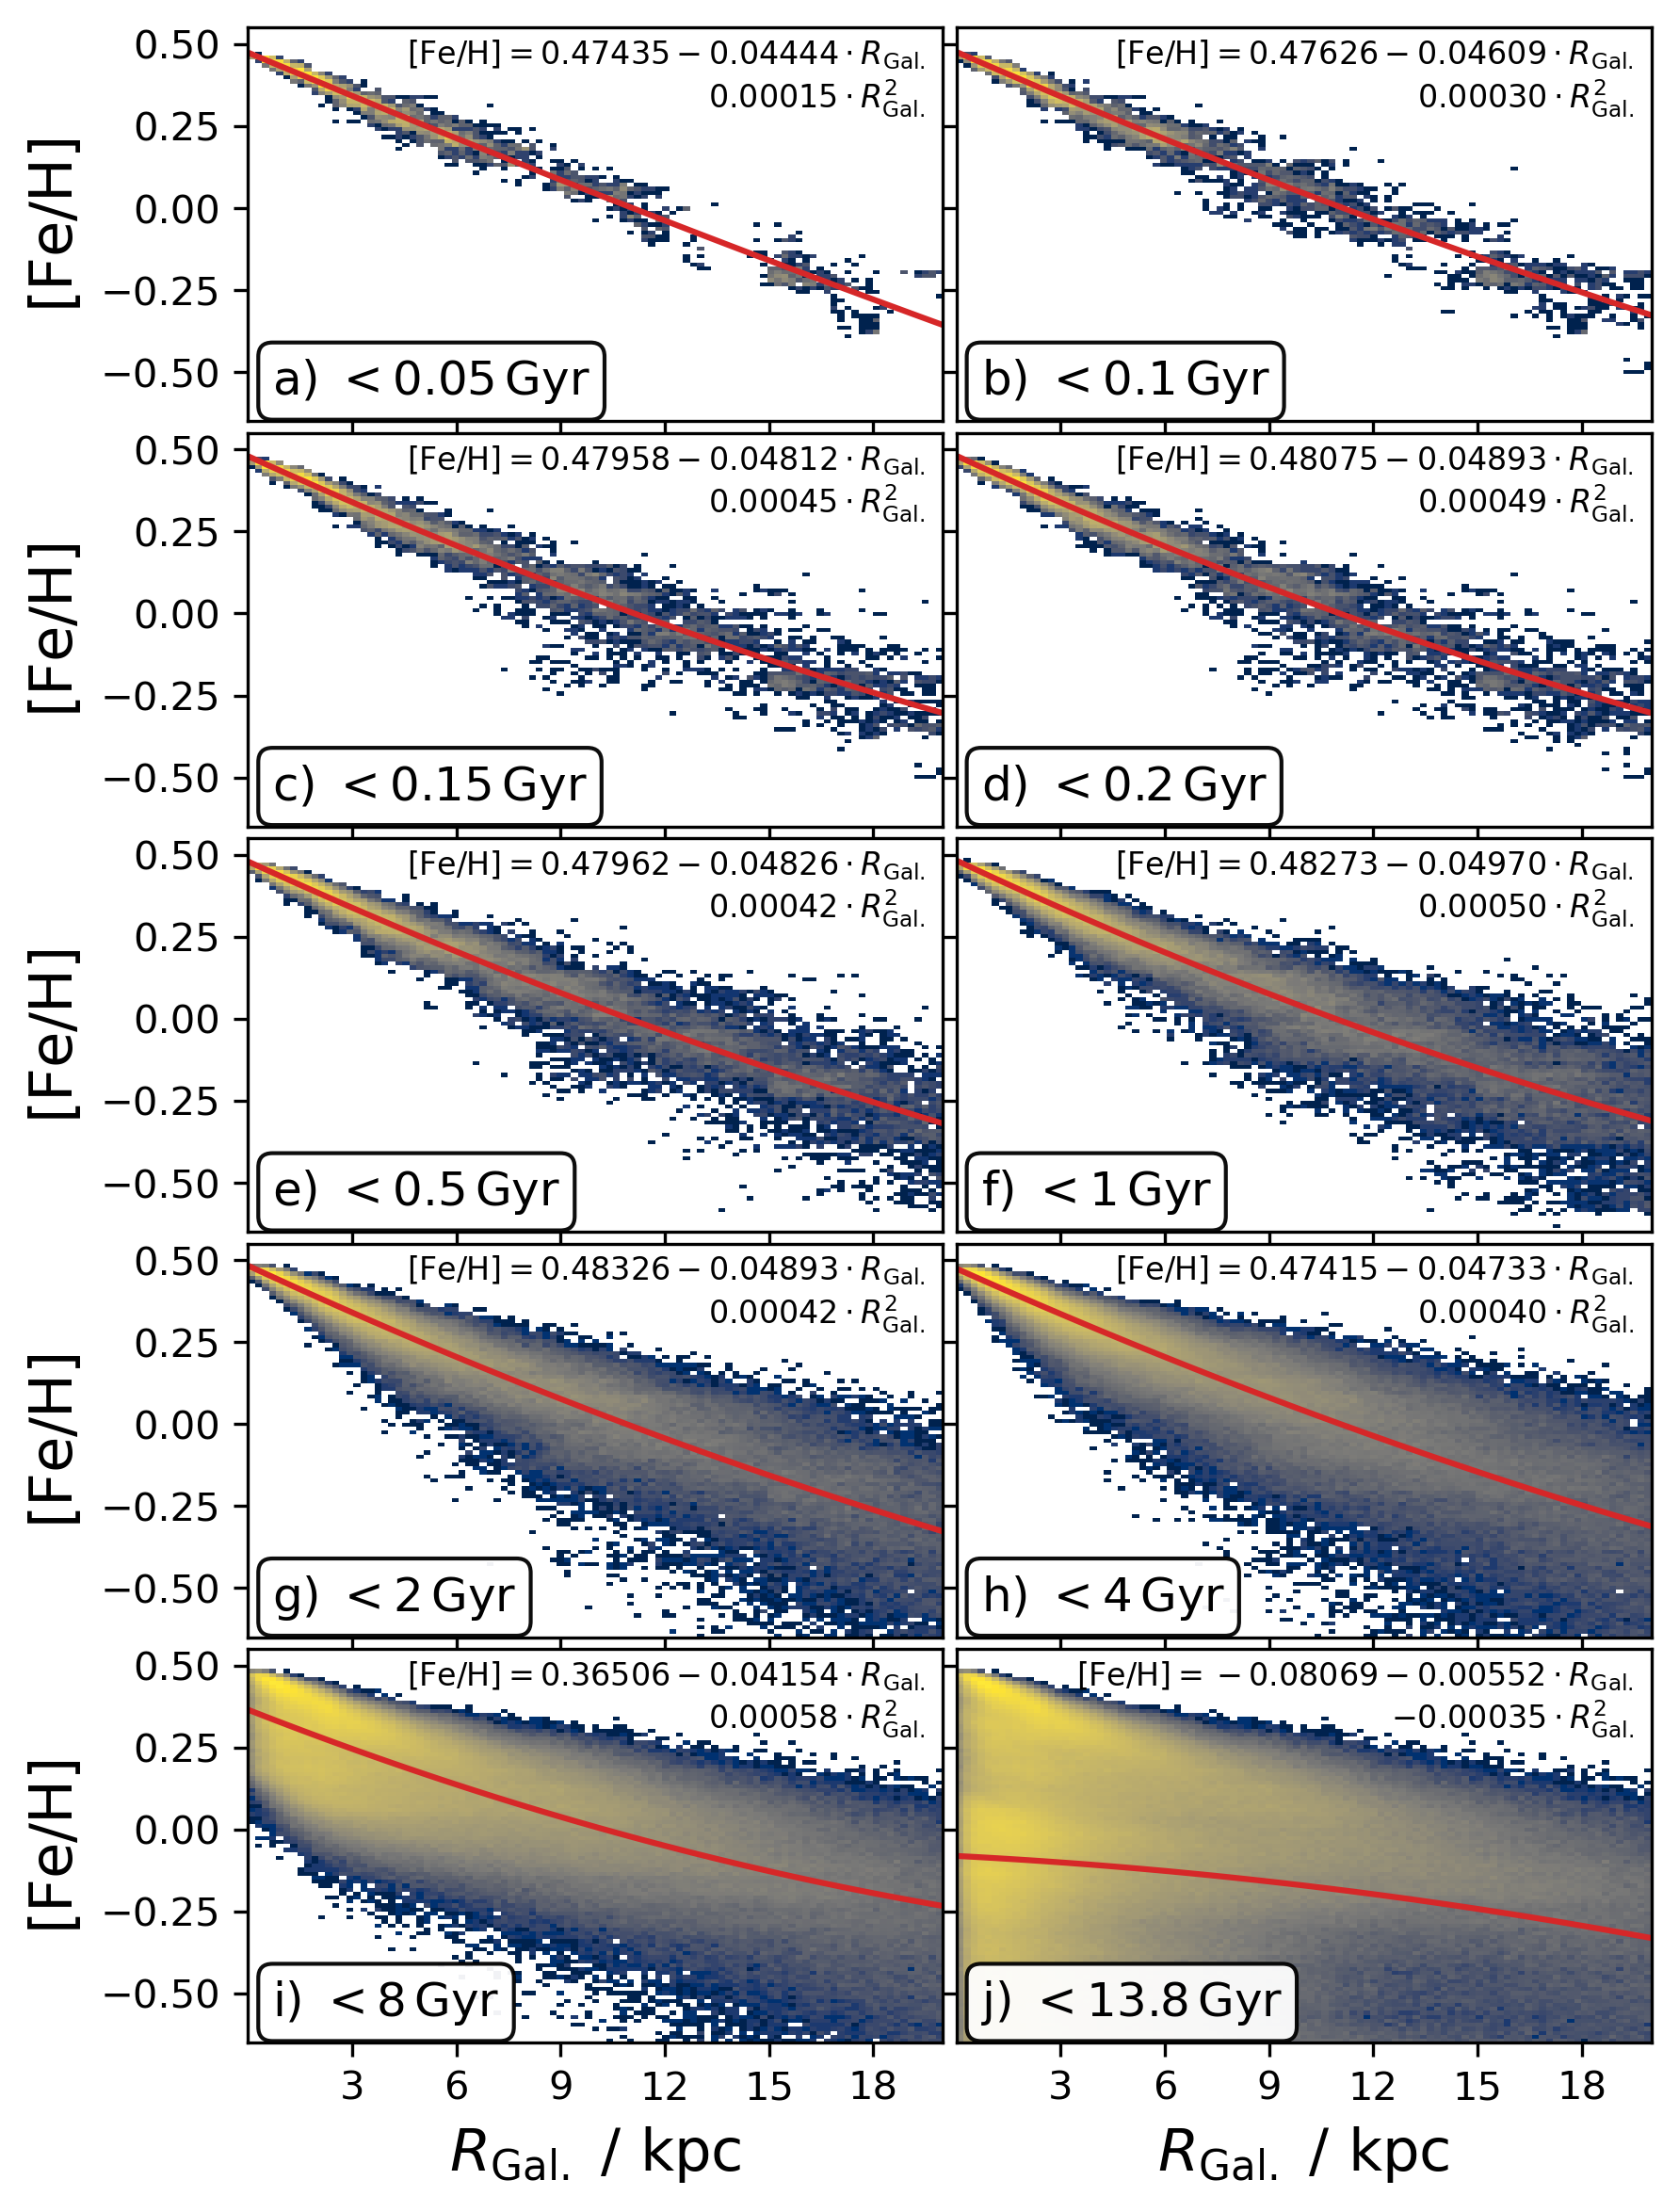
\includegraphics[width=\columnwidth]{figures/quadratic_fit_across_maximum_ages.png}
    \caption{Radial metallicity gradients and quadratic fits for different maximum age ranges.}
    \label{fig:quadratic_fit_across_maximum_ages}
\end{figure}



\begin{figure*}
    \centering
    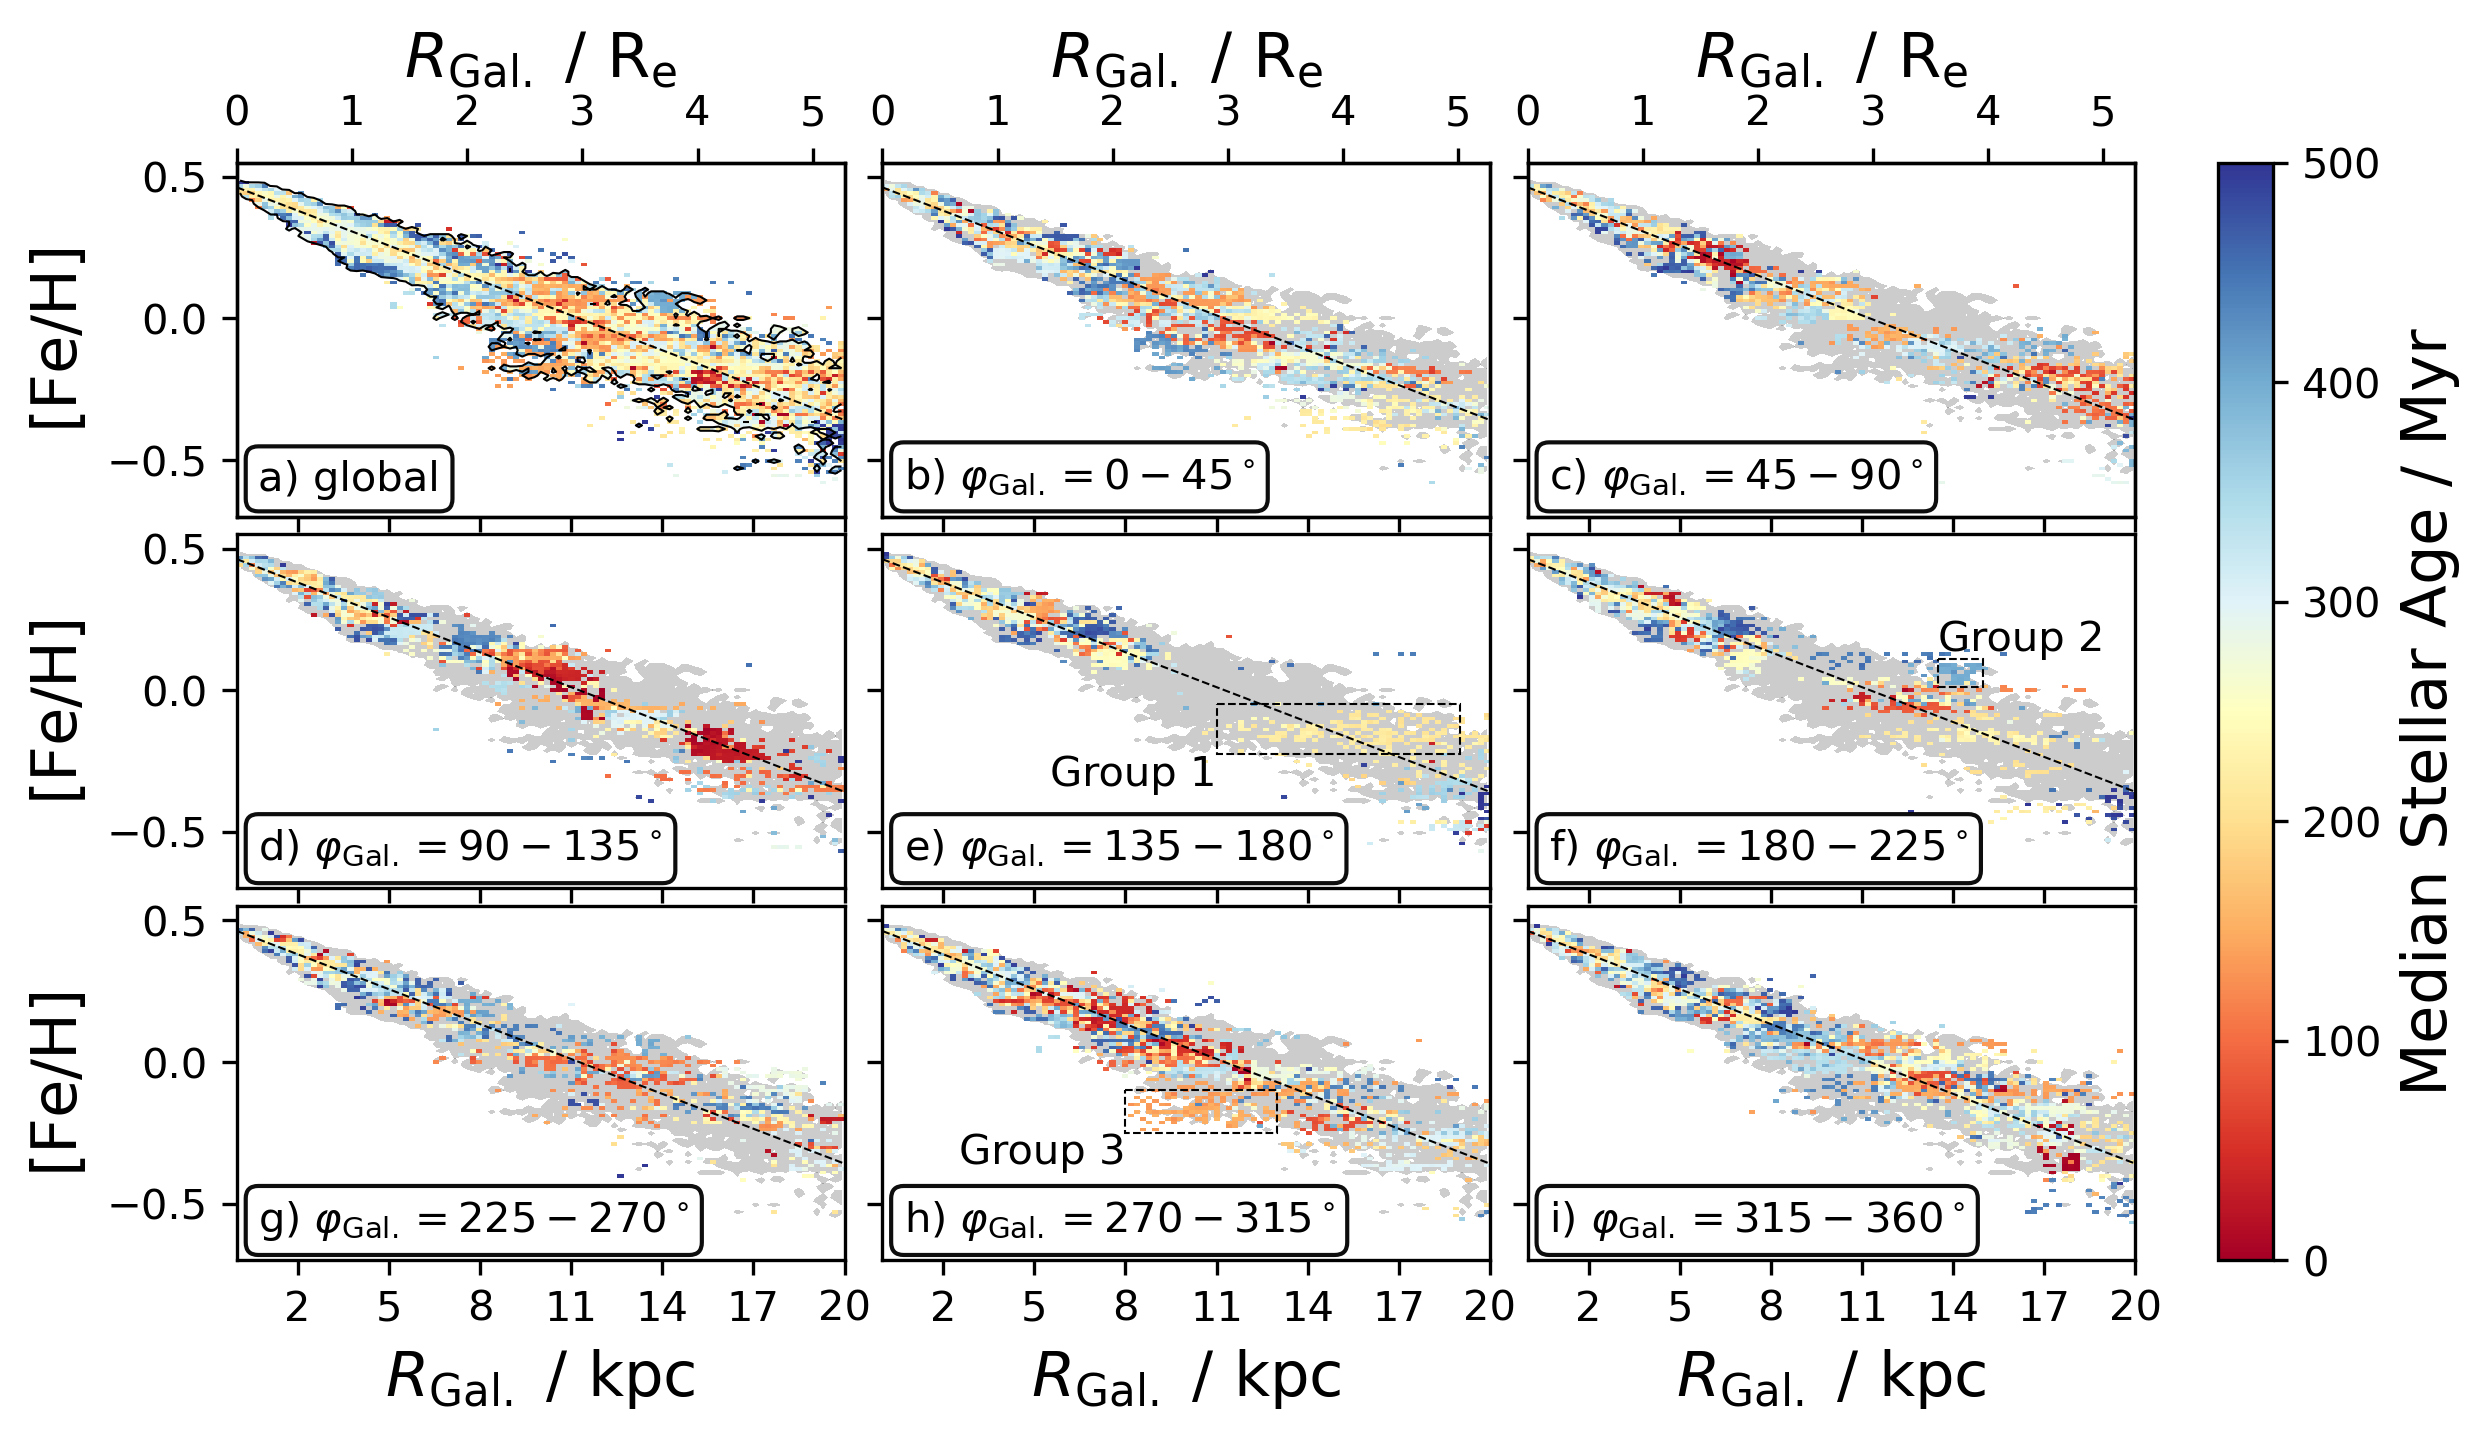
\includegraphics[width=\textwidth]{figures/radial_metallicity_gradients_mw_in_angles_age.png}
    \caption{Same as Fig.~\ref{fig:linear_radial_metallicity_gradients_mw_in_angles}, but colored by median age per bin. A rotating lighthouse-like GIF animation of the median age and median density of the $R-\mathrm{[Fe/H]}$-relation across different azimuths is freely available a \href{https://github.com/svenbuder/nihao_radial_metallicity_gradients/blob/main/figures/xyz_rfeh.gif}{repository}.}
    \label{fig:radial_metallicity_gradients_mw_in_angles_age}
\end{figure*}

\begin{figure}
    \centering
    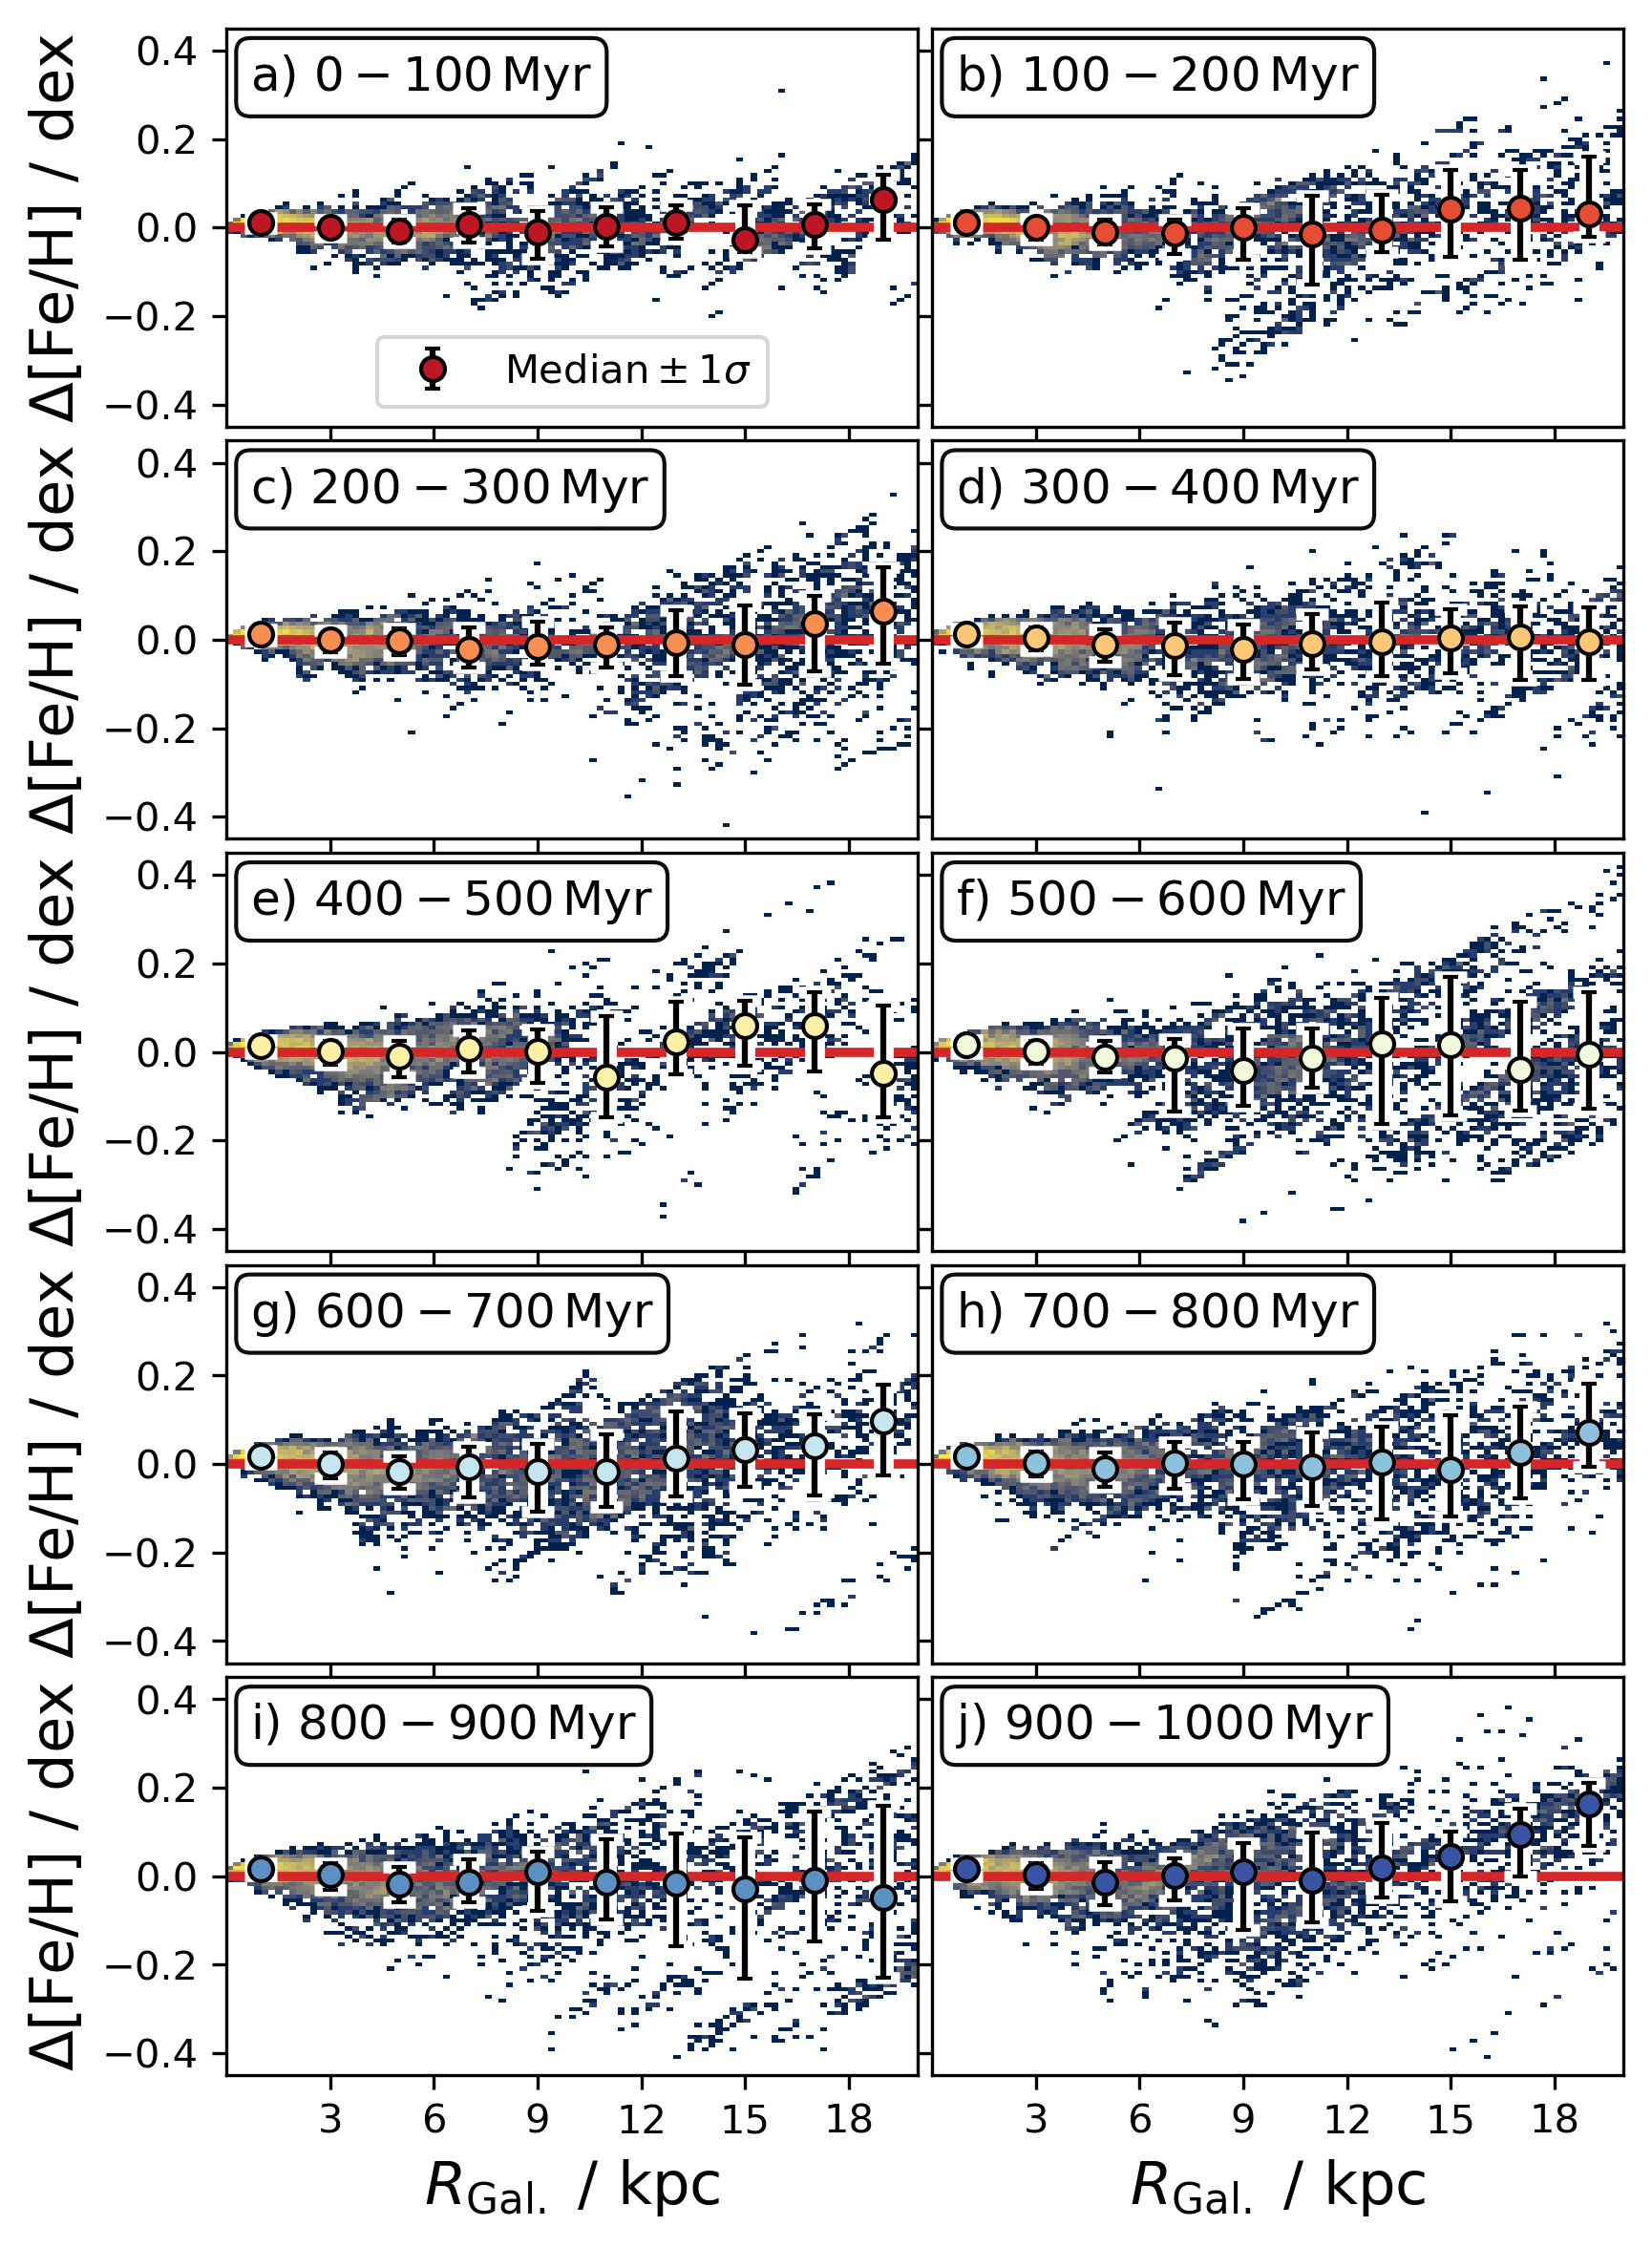
\includegraphics[width=\columnwidth]{figures/scatter_with_increasing_age.png}
    \caption{Stellar density distribution and spread of [Fe/H] across different galactocentric radii with respect to a global linear radial metallicity gradient across different age ranges. Panels a-j) show young stars and exhibit a rather similar trend, whereas the scatter increases significantly for stars above \nihaoAGEmax\ in panels panels k) and l).}
    \label{fig:scatter_with_increasing_age}
\end{figure}

\subsection{Young stars vs. gas}
\label{sec:young_stars_vs_gas}

After having investigated vertical and azimuthal variations of the gradient in Sections~\ref{sec:coherence_vertical_radial_metallicity_gradients} and \ref{sec:coherence_azimuth_radial_metallicity_gradients} as well as its change in smaller age steps in Section~\ref{sec:coherence_age_radial_metallicity_gradients}, we are now aiming to compare the gradient of the youngest stars to that of the gas in the galaxy at redshift zero.

\begin{itemize}
    \item Fig.~\ref{fig:overlap_local_variation_gas}
    \item Follow up Fig.~\ref{fig:tracing_young_stars_and_gas_in_angles} by looking at the stellar and gas [Fe/H] for these regions!
    \item Talk about significant overdensities in Fig.~\ref{fig:tracing_young_stars_and_gas_in_angles}, e.g. 7kpc for 0-45deg, 7, 11, 16 kpc for 135-180 or 9-11 for 270-315. Should we follow up the radial gas metallicity gradient as well?!
    \item Comparing Fig.~\ref{fig:tracing_young_stars_and_gas_in_angles} with Fig.~\ref{fig:linear_radial_metallicity_gradients_mw_in_angles}: overlap these figures? looks like sometimes the $\Delta z$ tracks the $\Delta\mathrm{[Fe/H]}$, e.g. panels f? Also in oposite direction with panels b and i. So maybe better trace $\Delta \vert z \vert$ vs. $\Delta \mathrm{[Fe/H]}$! Can we use this to identify a warp?
    \item Also include gas metallicity gradient: Fig.~\ref{fig:global_r_feh_fit_gas}. Gas gradient is interestingly more linear!
\end{itemize}

\begin{figure}
    \centering
    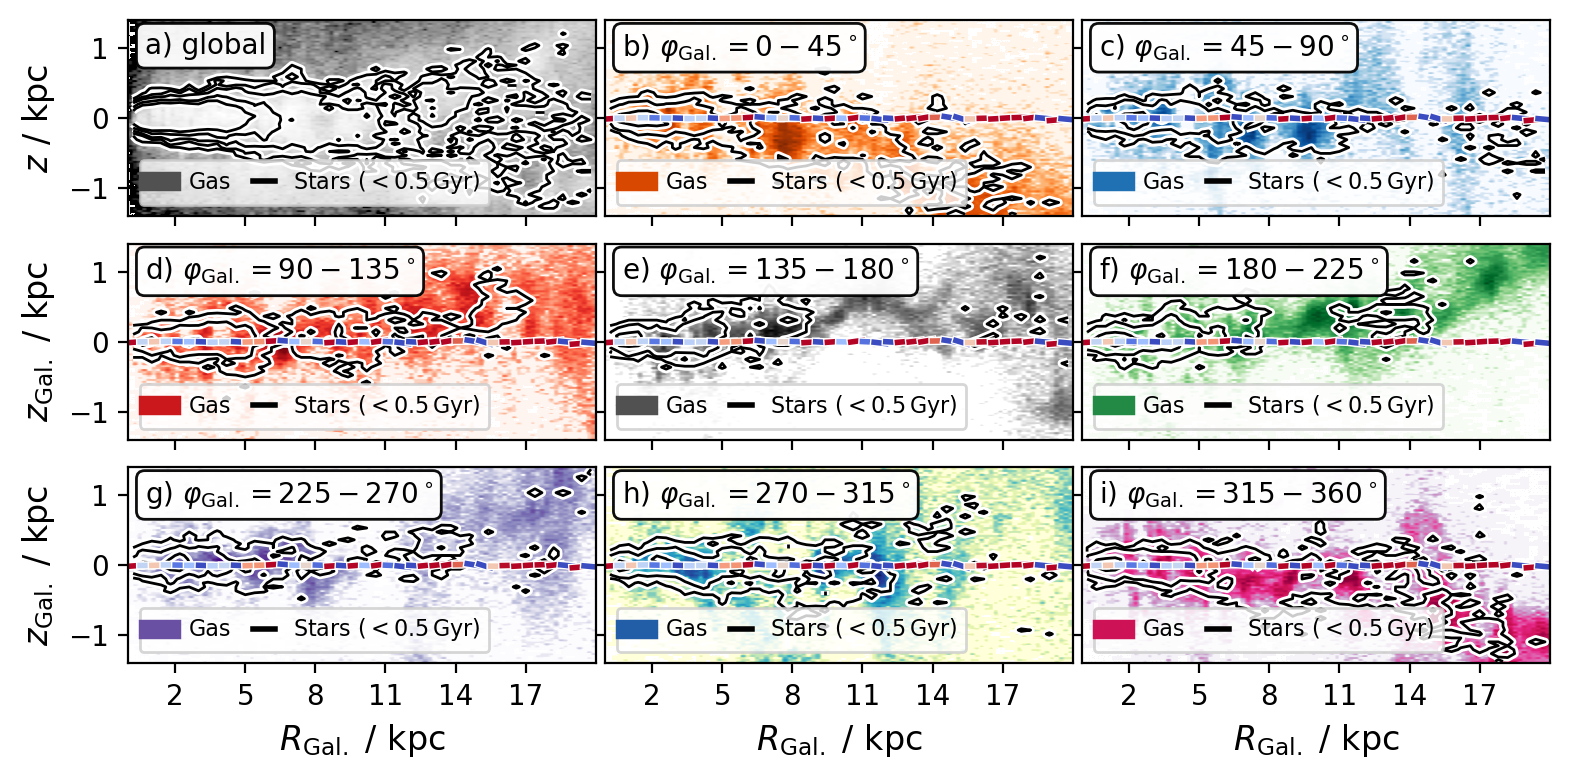
\includegraphics[width=\columnwidth]{figures/tracing_young_stars_and_gas_in_angles.png}
    \caption{Tracing young stars and gas across galactocentric radii $R_\mathrm{Gal.}$ and height $z_\mathrm{Gal.}$ across the whole galaxy (panel a) and different azimuthal ranges/sectors (panels b-i). Small rectangles with cool-warm colors along the horizontal axis indicate the local gradient slopes as in Fig.~\ref{fig:overlap_local_variation_gas}.}
    \label{fig:tracing_young_stars_and_gas_in_angles}
\end{figure}

\begin{figure}
    \centering
    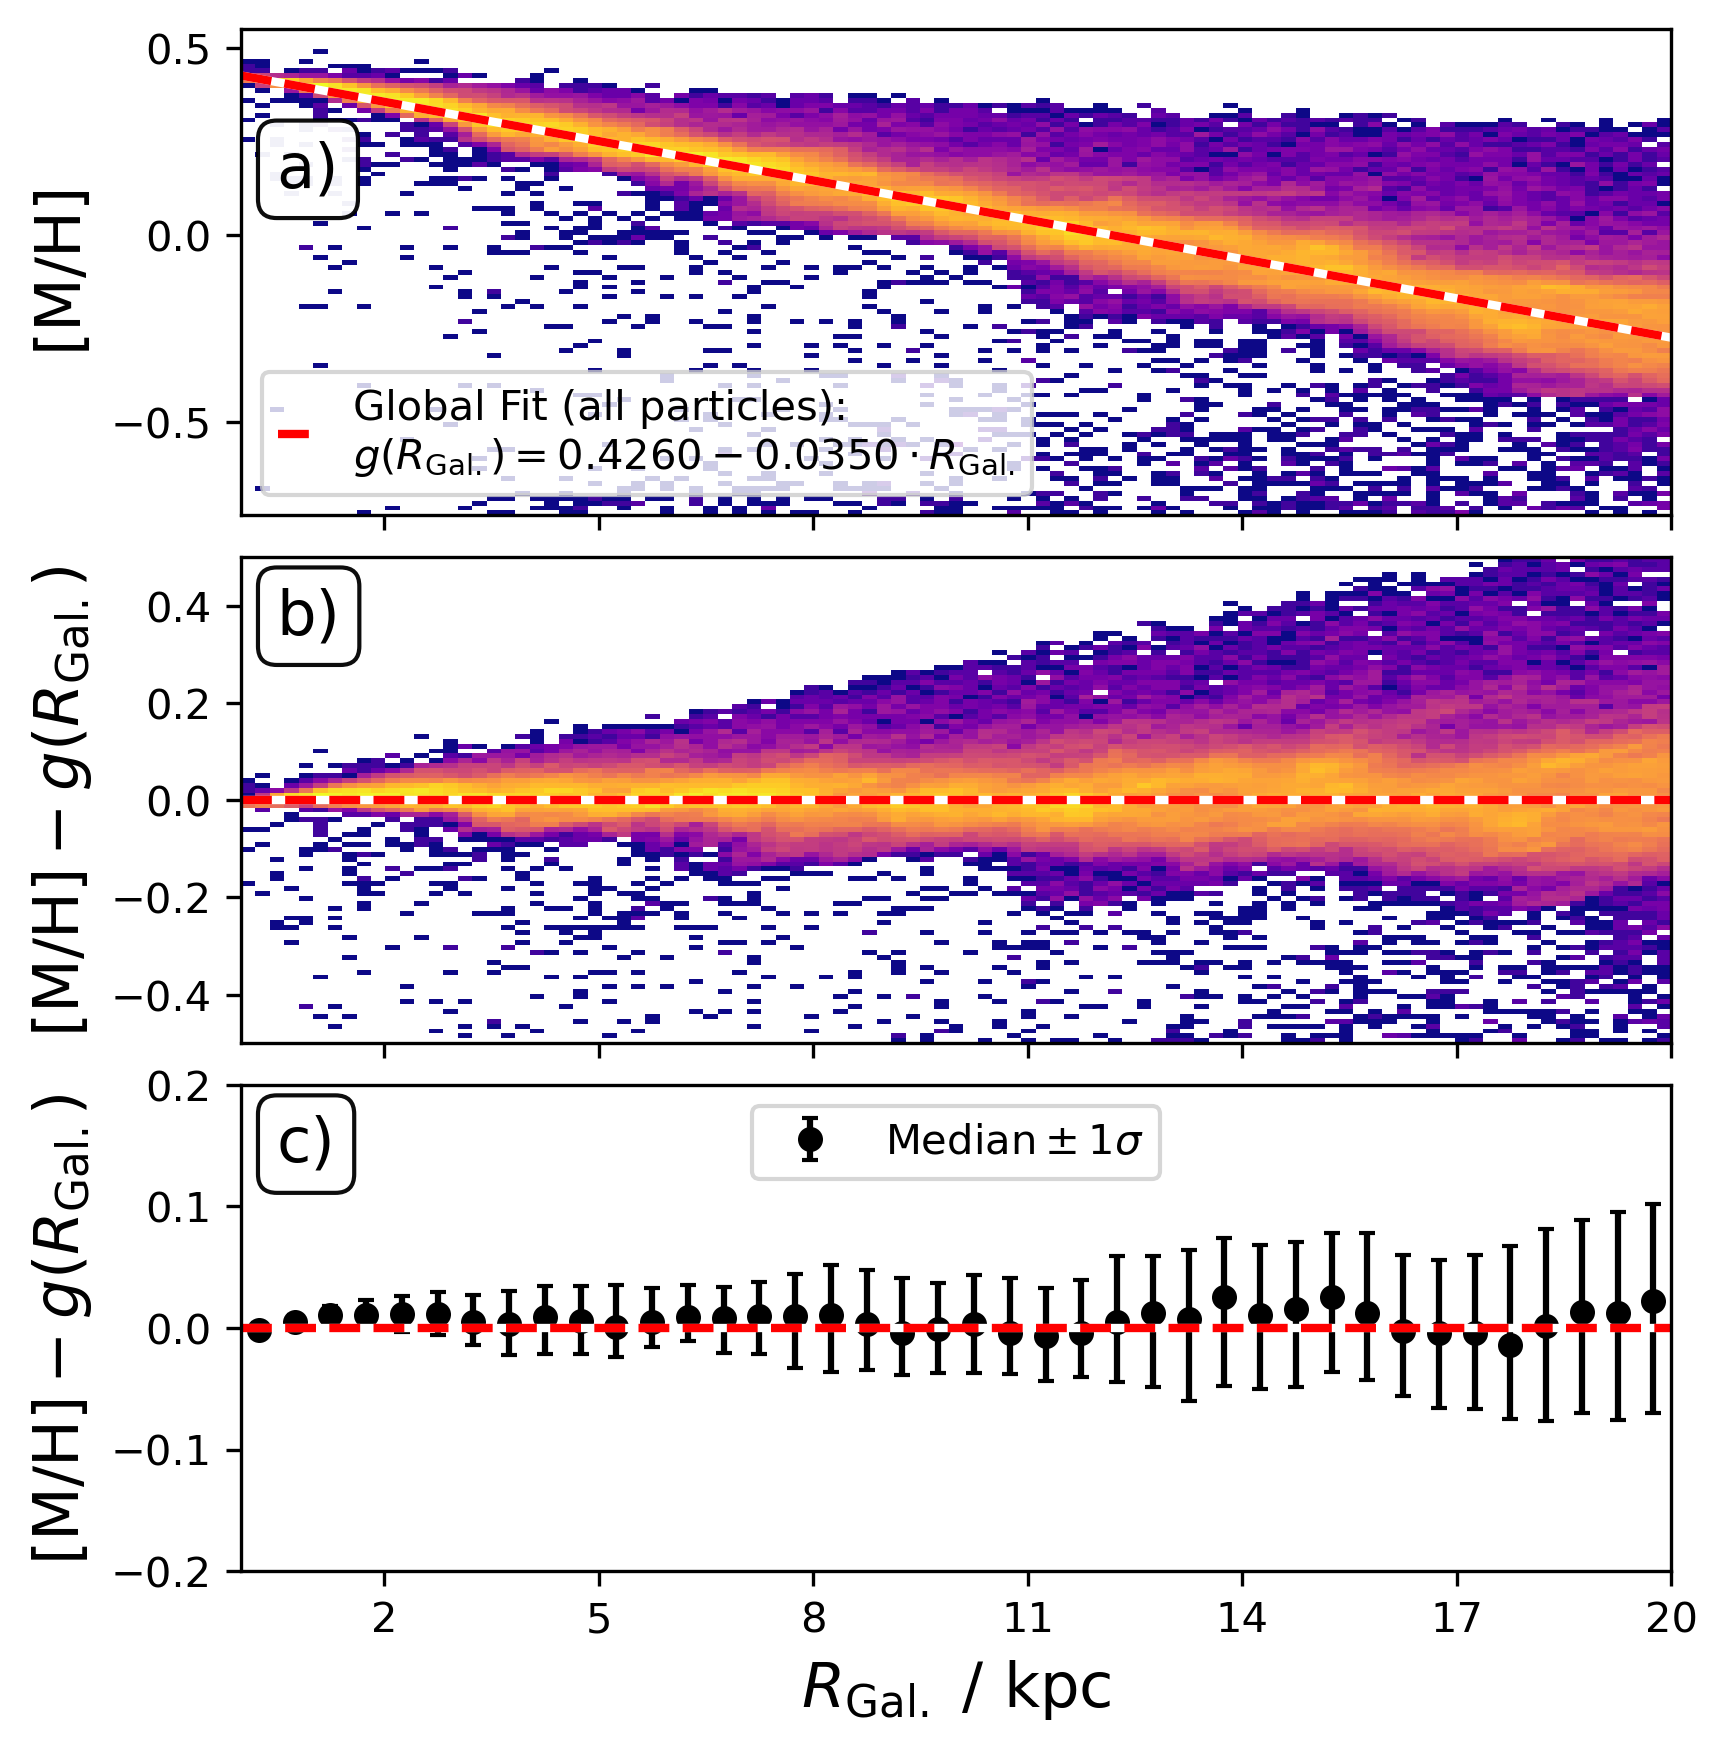
\includegraphics[width=\columnwidth]{figures/global_r_feh_fit_gas.png}
    \caption{Same as Fig.~\ref{fig:global_r_feh_fit}, but for gas.}
    \label{fig:global_r_feh_fit_gas}
\end{figure}

%%%%%%%%%%%%%%%%%%%%%%%%%%%%%%%%%%%%%%%%%%%%%%%%%%
\section{Discussion} \label{sec:discussion}

Comparison to \citet[][see their Fig. 10]{Minchev2014b}: They see significant decrease of stars towards larger radii (note to myself: their bins are not scatter, but number density in Fig. 10). How does this compare to our number densities?

\subsection{Linearity of the gradient} \label{sec:discussion_linearity}

\SB{How are the linear metallicity gradients usually measured? Any binning? If so, can we study what effect that has? How are uncertainties treated?}

To what extent is the radial metallicity gradient of young stars linear? Alternatively, would it be better described by two linear relations, with a break radius at corotation radius \citep[][and references therein]{Bresolin2012} or further out \citep{Donor2020} or a more sophisticated function \citep[see e.g.][]{Chiappini2001, Kubryk2015}? Investigating the gradient's form helps in understanding the galactic processes influencing metallicity at different radii \citep{Minchev2014b}.

\SB{"However, a simple, linear gradient may not be the better way to describe the distribution of the elements in the Galactic disk. From Cepheids, Andrievsky et al. (2002b), Pedicelli et al. (2009, 2010), and Genovali et al. (2013) found a steeper gradient in the very inner disk ($\leq 7\,\mathrm{kpc}$)." from \citet{Lemasle2013}}

\SB{"There are numerous abundance studies of open clusters from different groups: [...] They all reach the same conclusion: a linear gradient of approximately $-0.06\,\mathrm{dex/kpc}$ extending quite far into the outer disk, and a flattening at a level of $\mathrm{[Fe/H]} \approx -0.3\,\mathrm{dex}$, somewhere between 10 and 14 kpc." from \citet{Lemasle2013}.}

\SB{\citet{Lemasle2008} find $\mathrm{d[Fe/H]}/\mathrm{d}R = -0.050 \pm 0.008\,\mathrm{dex\,kpc^{-1}}$ in the 5-17 kpc range, but $\mathrm{d[Fe/H]}/\mathrm{d}R = -0.012 \pm 0.014\,\mathrm{dex\,kpc^{-1}}$ in a smaller 10-15 kpc range.}

\SB{How significant is the difference of linear to quadratic when looking at 5-19 kpc, like MW studies \citep{Genovali2014}?}

\SB{Put some of these results into context of the Milky Way in Fig.~\ref{fig:radial_metallicity_gradients_mw_vs_nihao}. Don't forget to cite all the people who contributed to the G+14 compilation, as well as Spina for GALAH and \citet{Myers2022, Donor2020} for APOGEE}

\begin{figure*}
    \centering
    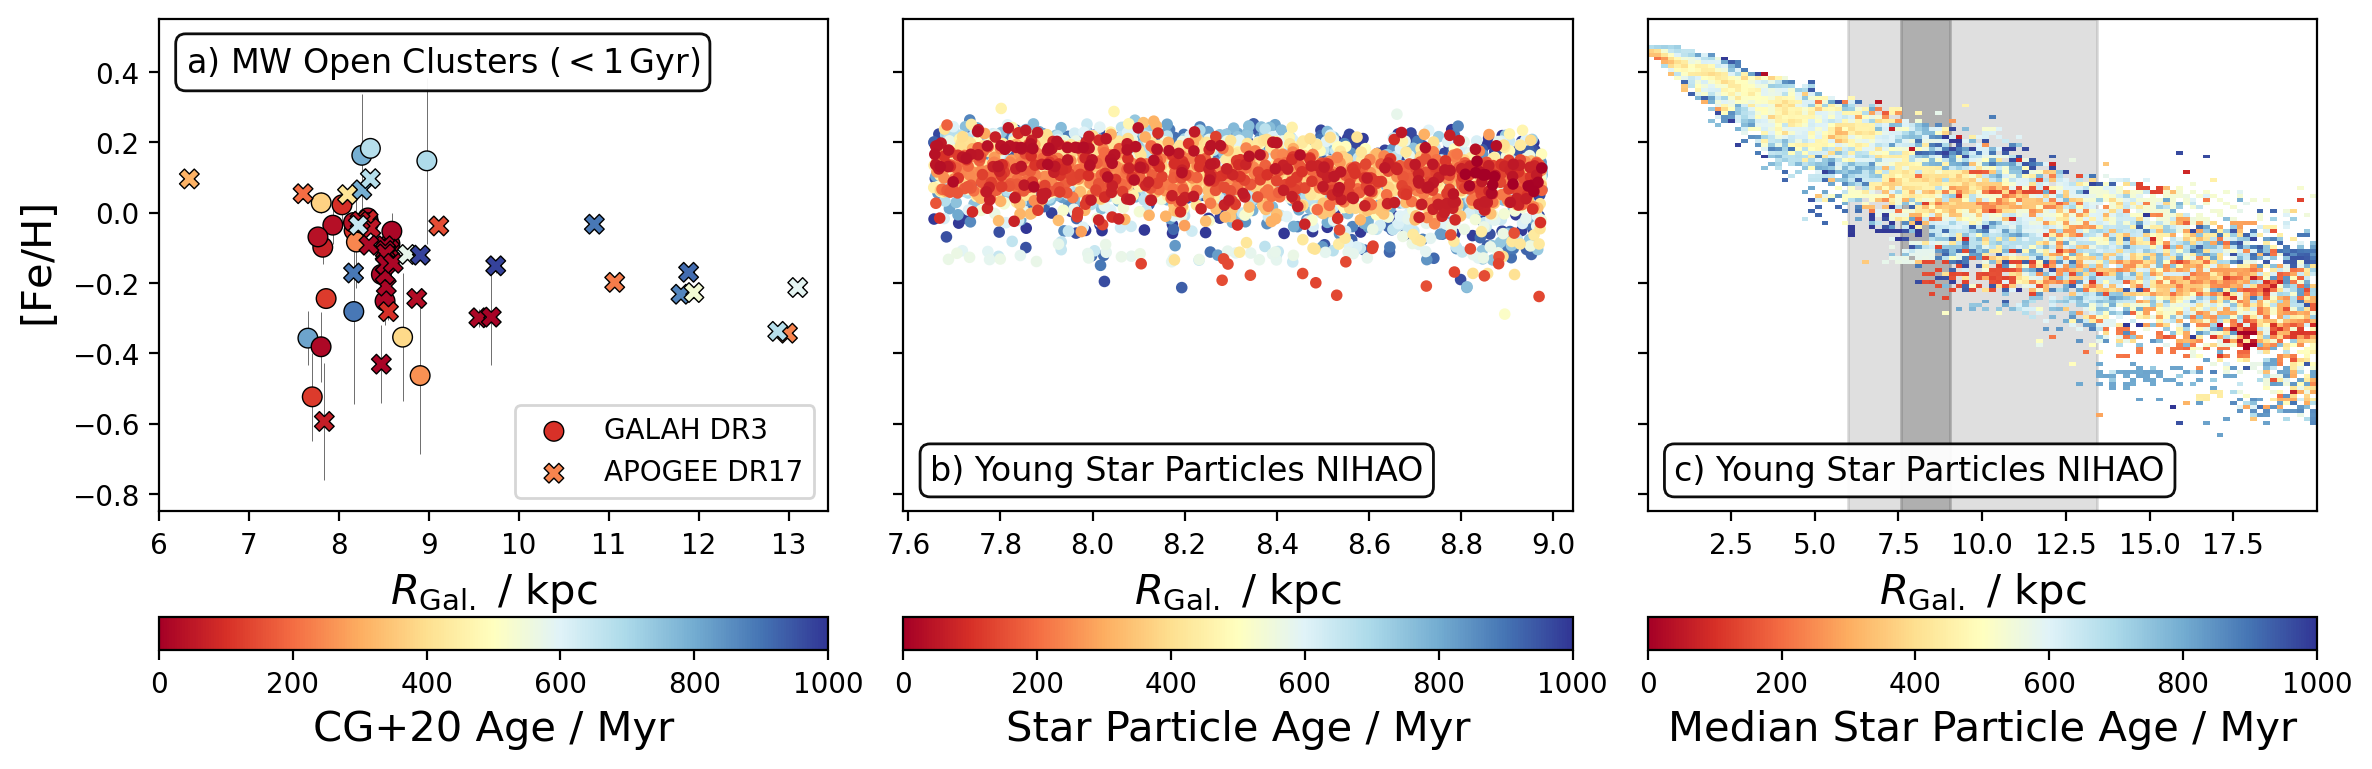
\includegraphics[width=\textwidth]{figures/radial_metallicity_gradients_mw_vs_nihao.png}
    \caption{Comparison of the Milky Way's radial metallicity trend as traced by Cepheids \citep[black triangles, compiled from literature by][G+14]{Genovali2014} as well as young ($<$\nihaoAGEmax) open cluster of the Milky Way as traced by the literature compilation from \citet[][G+14 as squares]{Genovali2014}, APOGEE DR17 from \citet[][M+22 as crosses]{Myers2022}, and GALAH DR3 from \citet[][S+21 as circles]{Spina2021}. The latter two are compiled based on the membership and age catalogue by \citet[][CG+20]{CantatGaudin2020}.
    }
    \label{fig:radial_metallicity_gradients_mw_vs_nihao}
\end{figure*}

\SB{Point out the low [Fe/H] outliers with ages below $200\,\mathrm{Gyr}$ in both observation (below $R_\mathrm{Gal.} < 10\,\mathrm{kpc}$ and $\mathrm{[Fe/H]} < -0.25$ in Fig.~\ref{fig:radial_metallicity_gradients_mw_vs_nihao}a) and simulation (few red dots around $\mathrm{[Fe/H]} \sim -0.15$ in Fig.~\ref{fig:radial_metallicity_gradients_mw_vs_nihao}c.}



\subsection{Scatter in the gradient} \label{sec:discussion_scatter}

How much scatter in the radial metallicity gradient of young stars is expected based on simulations? Quantifying the scatter can provide insights into the effects of transient events like mergers, star formation bursts, and gas accretion.

\SB{Put gas and star results into context of the Milky Way in Fig.~\ref{fig:overdensities_mw_vs_nihao}, inspired by \citet{Poggio2021} and \citet{Hackshaw2024}. We do not have enough star particles to really see substructure. But the gas shows similar substructure as the actual Milky Way.}

\begin{figure*}
    \centering
    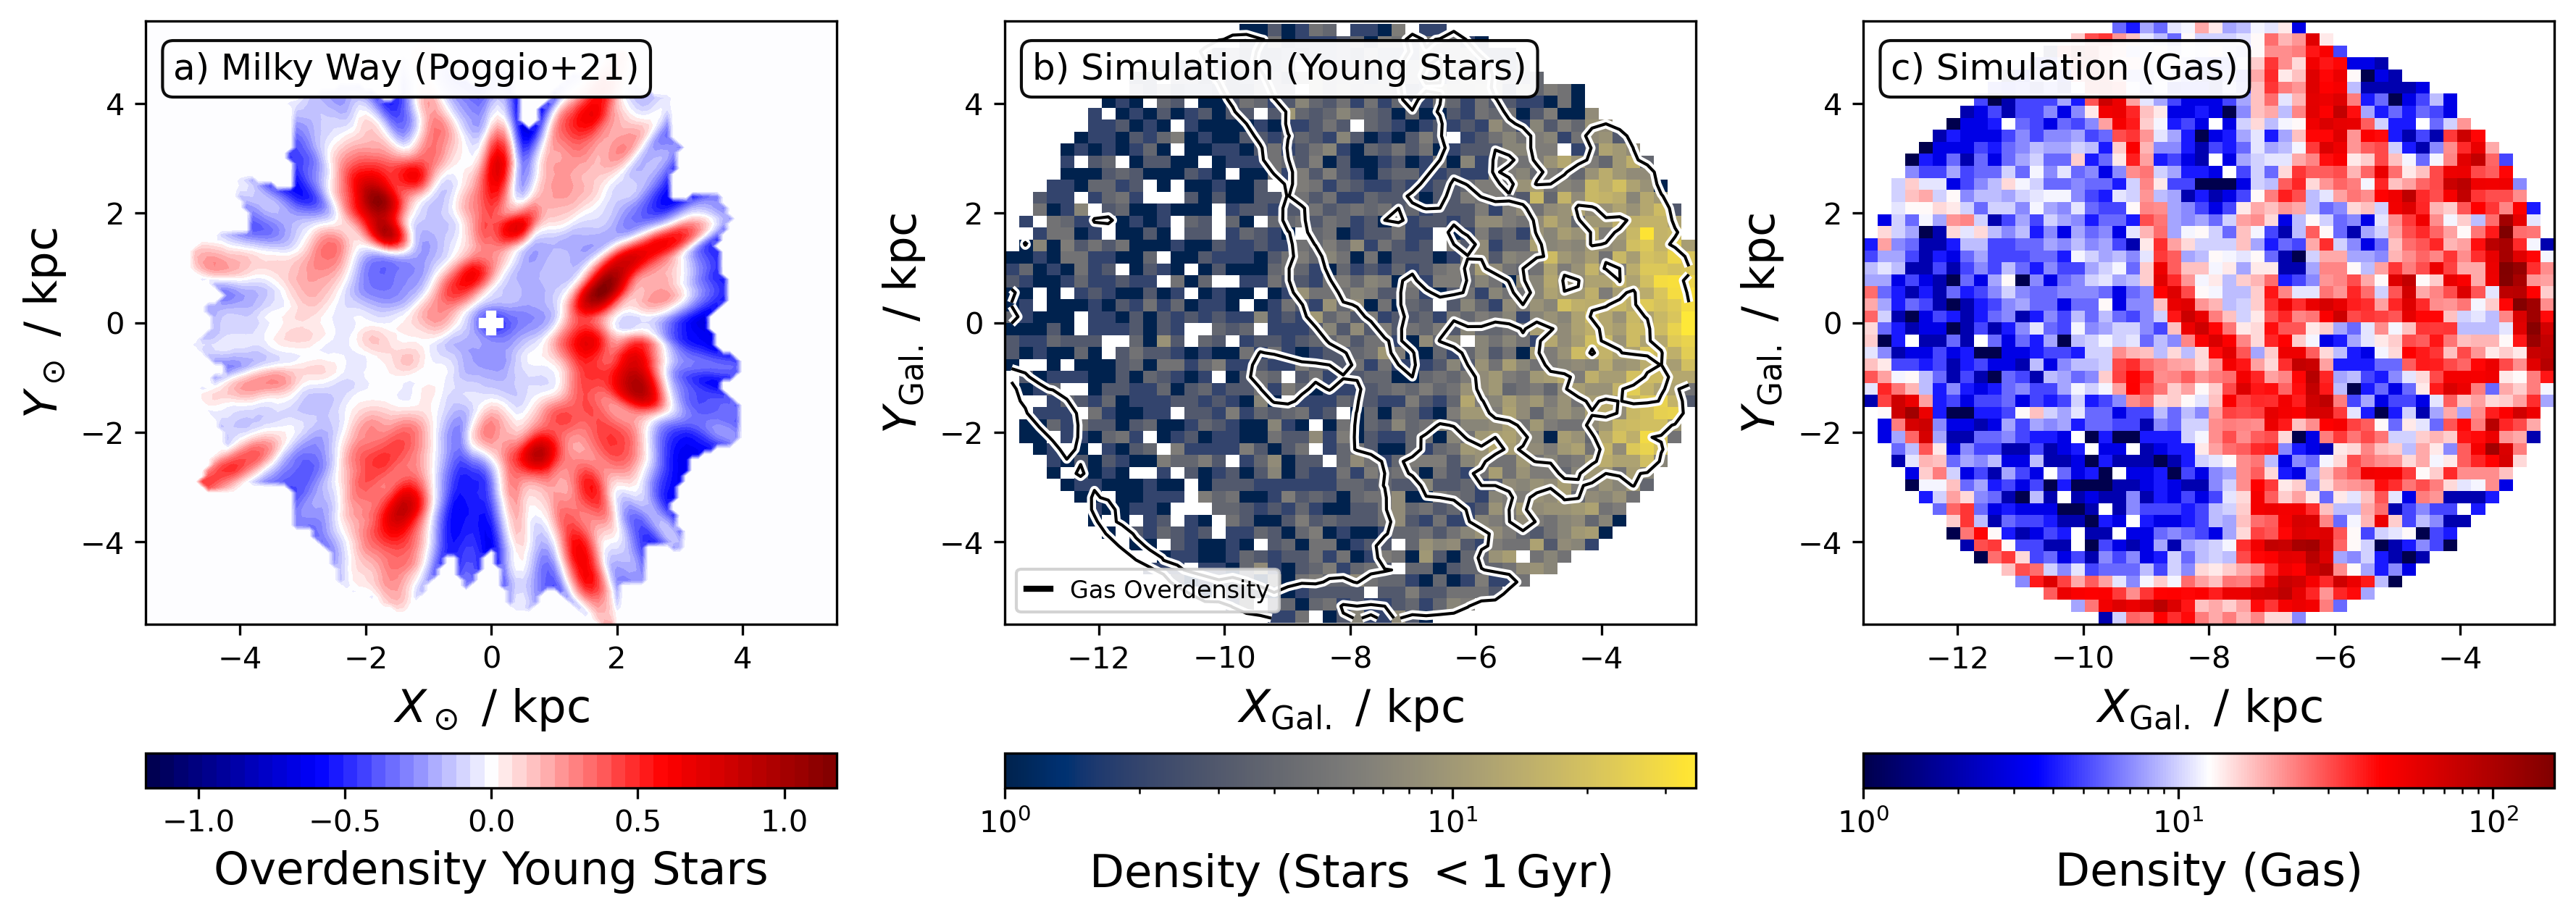
\includegraphics[width=\textwidth]{figures/overdensities_mw_vs_nihao.png}
    \caption{Comparison of density distribution of young stars and gas in the Milky Way and the NIHAO Milky Way analogue simulation. Panel a) shows the measurements of the Solar vicinity within $5\,\mathrm{kpc}$ by \citet{Poggio2021}. Panels b) and c) show young stars and gas NIHAO, respectively, for a selected region similar to panel a). Black and white contour lines in panel b) trace overdensities in the gas distribution of panel c).}
    \label{fig:overdensities_mw_vs_nihao}
\end{figure*}

\SB{How well can we resolve the differences of [Fe/H] in a similar regions as for the Milky Way? Fig.~\ref{fig:global_r_feh_fit_gas} shows this for gas and stars, respectively. Clear metallicity decrease in Fig.~\ref{fig:global_r_feh_fit_gas}a towards left (away from galactic centre). Residuals from linear gradient fit are more scattered towards left (away from galactic centre). Low number statistics (typically less than 5 particles per bin)? Gas (Fig.~\ref{fig:global_r_feh_fit_gas}c) also show lower iron abundances with increasing distance from centre. However, it is significantly more nuanced and shows step-like behaviour of [Fe/H] changes around edges of gas overdensities. Significant deviations from global gradient expectation especially in the large void around $-12 < X_\mathrm{Gal} < -10\,\mathrm{kpc}$. Follow-up would be interesting but is beyond scope of this paper.}

\SB{Fig.~\ref{fig:nihao_gas_stars_density_overlay}: put this into context of finding by \citet{Grand2016}: "Owing to the negative radial metallicity gradient, this systematic motion drives, at a given radius, an azimuthal variation in the residual metallicity that is characterized by a metal-rich trailing edge and a metal-poor leading edge."}

\begin{figure*}
    \centering
    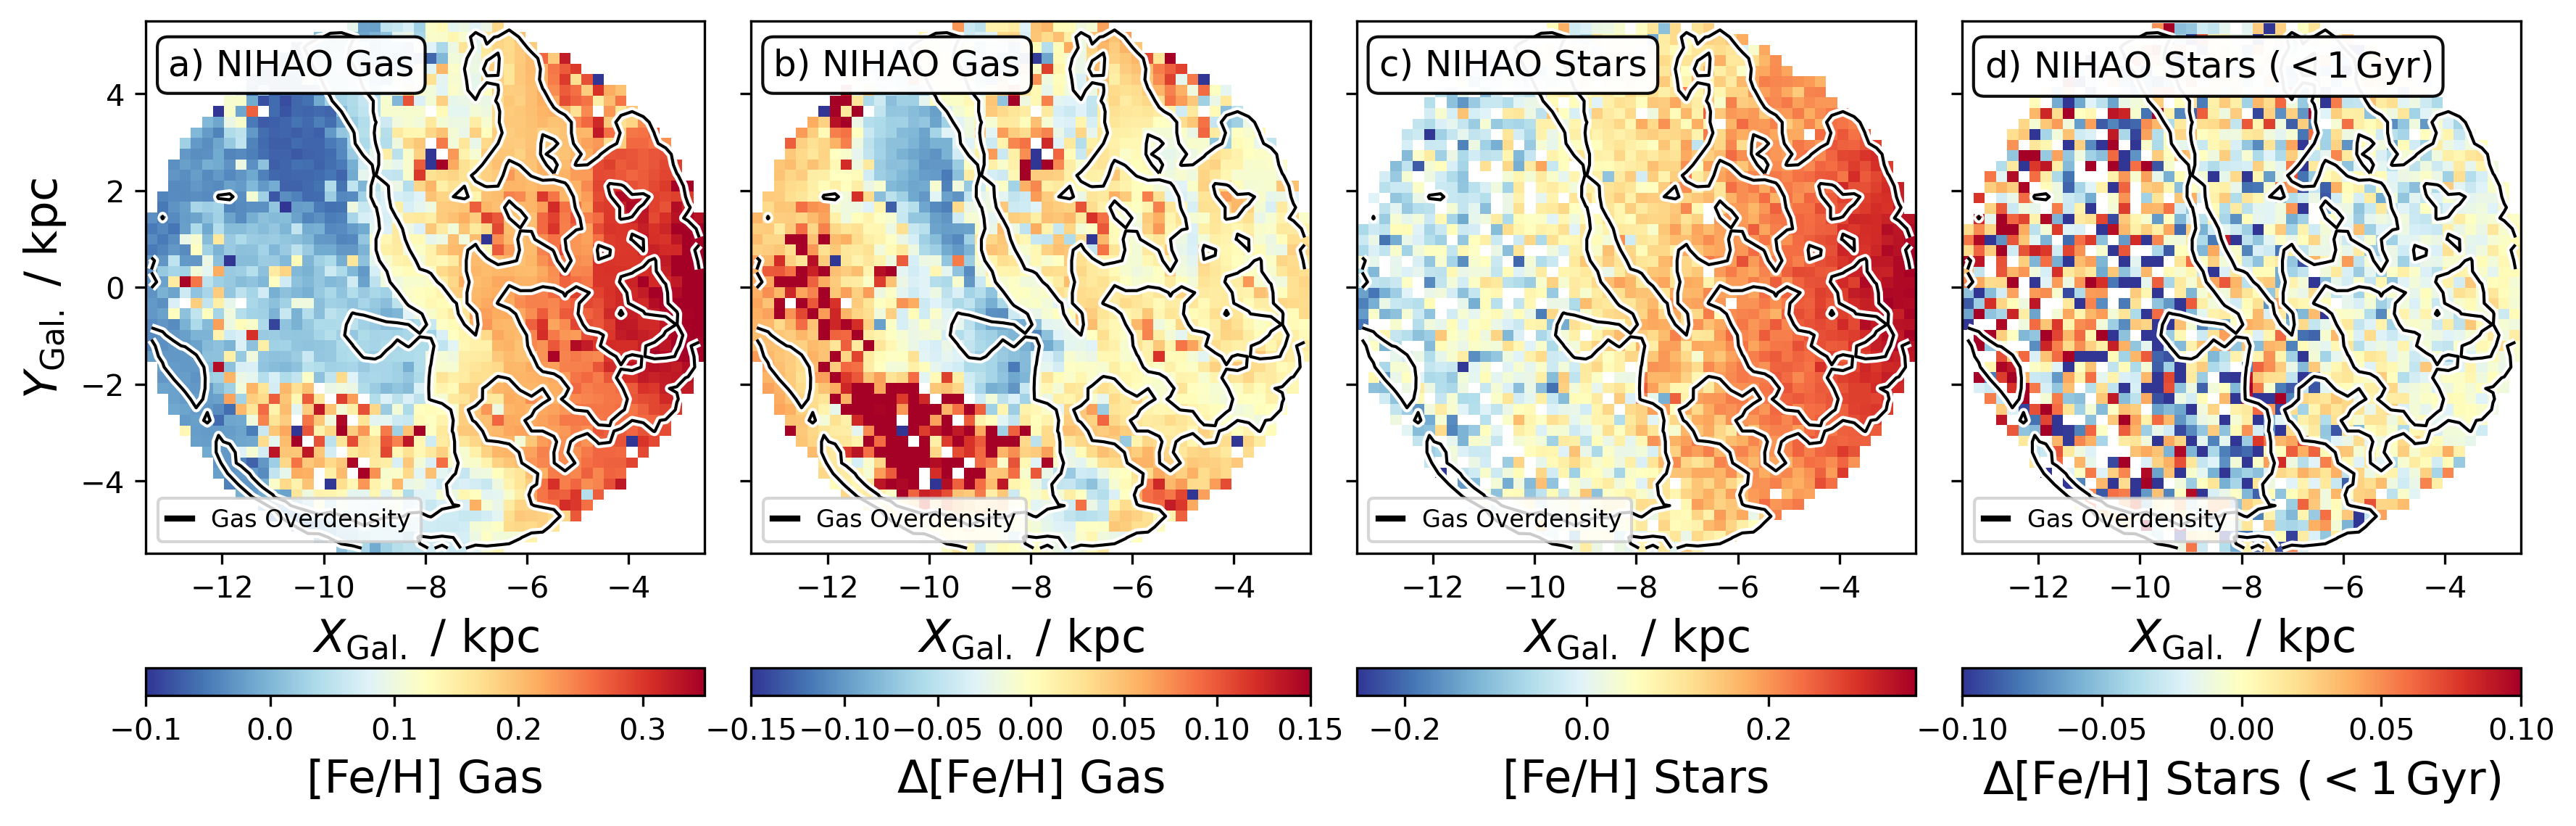
\includegraphics[width=\textwidth]{figures/nihao_gas_stars_density_overlay.png}
    \caption{Comparison of density distribution of young stars and gas NIHAO Milky Way analogue simulation for the same regions as Figs.~\ref{fig:overdensities_mw_vs_nihao}b and \ref{fig:overdensities_mw_vs_nihao}c. Panels a) and c) trace median gas and young star iron abundances, respectively. Panels b) and c) plot the residual [Fe/H] of gas and stars, respectively, when correcting with a radial metallicity gradient fit. Black and white contour lines in panel b) trace overdensities in the gas distribution of Fig.~\ref{fig:overdensities_mw_vs_nihao}c).}
    \label{fig:nihao_gas_stars_density_overlay}
\end{figure*}


\subsection{Coherence of the gradient with position} \label{sec:discussion_coherence_position}

How significant is the change in the radial metallicity of young stars gradient as a function of position, both in terms of radial coverage and azimuth? Understanding these variations can reveal the underlying processes affecting metallicity distribution, such as spiral arm dynamics and bar-driven mixing \citep[see their Figs. 5-8][]{DiMatteo2013}.

\subsection{Coherence of the gradient with age} \label{sec:discussion_coherence_age}

Until what stellar age can stars be used as reliable tracers of the gas disk in simulations, in terms of both chemical composition and position? This question is pivotal for interpreting observed gradients across different ages \citep[e.g.][]{Willett2023} and comparing them with model predictions, particularly concerning the migration and heating of stellar populations \citep{Binney2008, Frankel2018}.

Radial migration?
\begin{itemize}
    \item \citet{Grand2016} as recommended by Qian-Hui.
\end{itemize}

\subsection{The connection of young stars and gas}

\begin{itemize}
    \item Discuss both Fig.~\ref{fig:tracing_young_stars_and_gas_in_angles} and Fig.~\ref{fig:global_r_feh_fit_gas}
    \item Gas-phase metallicity break in IllustrisTNG \citep{Hemler2021, Garcia2023}?
    \item compare quadratic profiles we find to the flattening profiles in Fig.~4 by \citet{Hemler2021}, which resemble decreasing, flattening quadratic or inverse proportional ($\propto R_\mathrm{Gal.}^{-1}$) shapes. See also Fig.~4 by \citet{Garcia2023}.
    \item Flattening due to N/O \citep{Grasha2022}, constant below $\mathrm{A(O)} \sim 8.0$? -> compare to Fig.~\ref{fig:trace_stars_and_gas_100kpc}d -> in turn compare to young thin disk stars being born with with lower metallicity due to inside-out metallicity enhancement.
\end{itemize}

\subsection{Application of quadratic gradient function onto observations}

\begin{itemize}
    \item Can we apply our functional form onto MW data? e.g. \citet{Yong2012, Andrievsky2004, Genovali2014}?
    \item Can we apply our functional form onto extragalactic data? e.g. \citet{Chen2023, Bresolin2012}?
\end{itemize}

\citet{Sanchez2014} analysed a sample of 306 galaxies and found that breaks in metallicity gradients are common in both spiral and barred galaxies, often occurring at radii between 1 and 2 effective radii (Re): "Beyond $\sim 2$ disk effective radii our data show evidence of a flattening in the abundance"

Using data from the MaNGA survey, \citet{Belfiore2017} found that many galaxies exhibit breaks in their metallicity gradients: "At large radii, a flattening of the metallicity gradient with respect to the value $0.5 < R/R_e < 2.0$ is detected for $\log10(M_\star/M_\odot) > 9.5$, although with varying degrees of significance. " \SB{look into their text on the shape and description of the flattening!}

\citet{Bresolin2012} break in gradient for M83, NGC 1512, NGC3621, and NGC4625.
\citet{Vlajic2009} maybe most reasonable fit with 2 lines and a break radius for NGC 300.

\SB{this NIHAO galaxy has a strong warp \citep[compared to other NIHAO-UHD simulations][]{Buck2020}. How does the metallicity gradient look like for other galaxies without a warp?!}

\subsection{Limitations}

\begin{itemize}
    \item Outer break radius for Milky Way with stellar mass $\log(M_\star/\mathrm{M_\odot} = 10.7$ \citep{BlandHawthorn_Gerhard2016} at redshift $z \sim 0$ would be expected to be roughly around $25-35\,\mathrm{kpc}$ based on IllustrisTNG simulations \citep[][their Appendix A]{Garcia2023}.
    \item By going beyond the typically traced radii of around $20\,\mathrm{kpc}$, we trace the limitations of our findings for the outskirts of a galaxy. In Fig.~\ref{fig:trace_stars_and_gas_100kpc}, we are tracing all stars, young stars, and all gas out to $R_\mathrm{Gal.} \leq 100\,\mathrm{kpc}$, as done by \citet{Garcia2023} for IllustrisTNG. We also restrict our sample to $\vert z_\mathrm{Gal.} \vert \leq 50\,\mathrm{kpc}$, neglecting a smaller ($M_\star = 1.4\cdot 10^8\,\mathrm{M_\odot}$) galaxy around (X,Y,Z) = $(0,60,190)\,\mathrm{km\,s^{-1}}$, that is, $200\,\mathrm{kpc}$ distance.
\end{itemize}

\begin{figure}
    \centering
    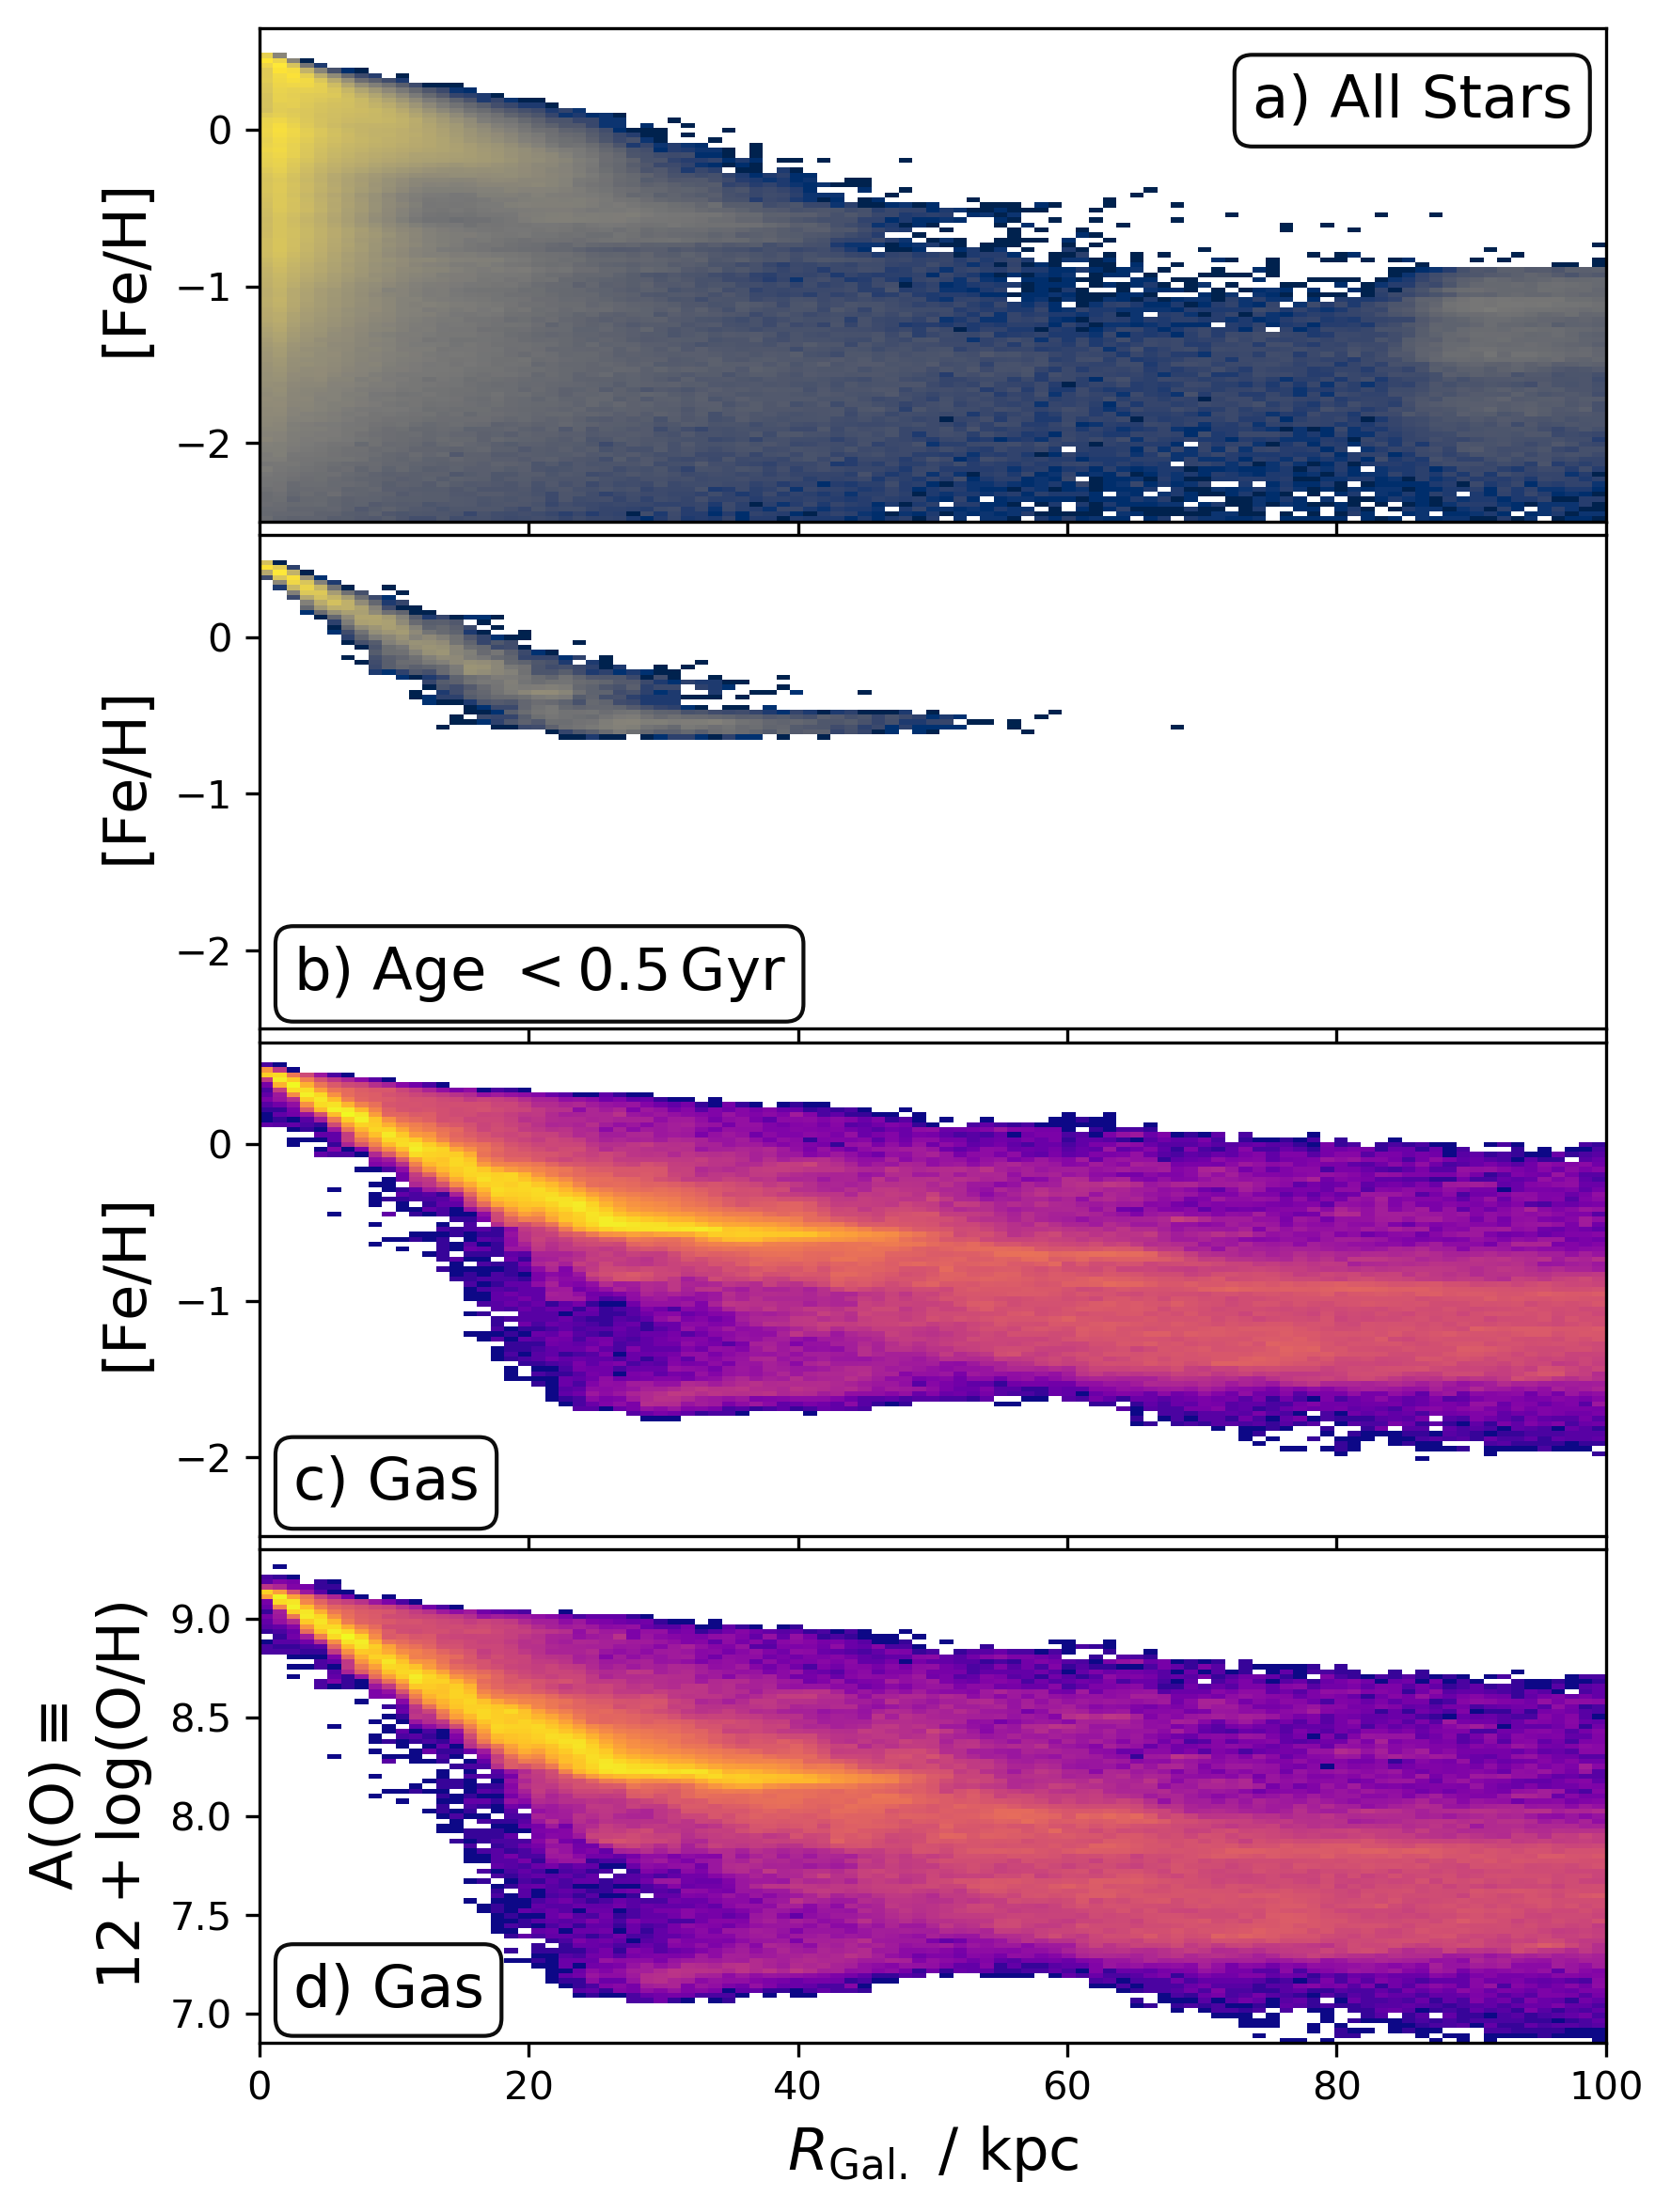
\includegraphics[width=\columnwidth]{figures/trace_stars_and_gas_100kpc.png}
    \caption{Radial metallicity functions for all stars (panel a), young stars (panel b), and gas (panels c and d for iron and oxygen as metallicity tracers) out to $R_\mathrm{Gal.} \leq 100\,\mathrm{kpc}$. Panels b and c are comparable to Figs.~\ref{fig:global_r_feh_fit}a and \ref{fig:global_r_feh_fit_gas}a for a smaller radial coverage.}
    \label{fig:trace_stars_and_gas_100kpc}
\end{figure}

%%%%%%%%%%%%%%%%%%%%%%%%%%%%%%%%%%%%%%%%%%%%%%%%%%
%%%%%%%%%%%%%%%%%%%%%%%%%%%%%%%%%%%%%%%%%%%%%%%%%%
\section{Conclusions}
\label{sec:conc}

\subsection{Main Take-Away}

\subsection{Future Research}

\begin{itemize}
    \item Can we say what the linear gradient and flattening part is for $R_\text{eff}$ for our NIHAO Milky Way analogue. Can we relate this to the MW effective radius and other galaxies?
\end{itemize}

\section*{Acknowledgements}

\begin{CJK}{UTF8}{gbsn}
We thank Kathryn Grasha and Qian-Hui Chen (陈千惠) for valuable discussions.
\end{CJK}

We acknowledge the traditional owners of the land on which the ANU stands, the Ngunnawal and Ngambri people. We pay our respects to elders past, and present and are proud to continue their tradition of surveying the night sky and its mysteries to better understand our Universe.

This work was supported by the Australian Research Council Centre of Excellence for All Sky Astrophysics in 3 Dimensions (ASTRO 3D), through project number CE170100013. SB acknowledges support from the Australian Research Council under grant number DE240100150 which enabled SB to continue researching at the end of a fixed-term position and finalising this study. TB acknowledges funding from the Carl Zeiss Stiftung and support from the European Research Council under ERC-CoG grant CRAGSMAN-646955. We gratefully acknowledge the Gauss Centre for Supercomputing e.V. (\url{www.gaus s-centre.eu}) for funding this project by providing computing time on the GCS Supercomputer SuperMUC at Leibniz Supercomputing Centre (\url{www.lrz.de}). Simulations were partially computed with High Performance Computing resources at New York University, Abu Dhabi.

\section*{Software}

The research for this publication was coded in \textsc{python} (version 3.7.4) and included its packages
\textsc{astropy} \citep[v. 3.2.2;][]{Robitaille2013,PriceWhelan2018},
\textsc{IPython} \citep[v. 7.8.0;][]{ipython},
\textsc{matplotlib} \citep[v. 3.1.3;][]{matplotlib},
\textsc{NumPy} \citep[v. 1.17.2;][]{numpy},
\textsc{pynbody} \citep[v. 1.1.0;][]{pynbody},
\textsc{scipy} \citep[v. 1.3.1;][]{Scipy},
\textsc{sklearn} \citep[v. 1.5.1][]{scikit-learn}
\textsc{statsmodels} \citep[v. 0.14.2][]{statsmodels}
We further made use of \textsc{topcat} \citep[version 4.7;][]{Taylor2005};

%%%%%%%%%%%%%%%%%%%%%%%%%%%%%%%%%%%%%%%%%%%%%%%%%
\section*{Data Availability}

All code and data to reproduce the analysis and figures can be publically accessed via \url{https://github.com/svenbuder/nihao_radial_metallicity_gradients}.

% The repository also includes the chemical and kinematic data of the simulated Milky Way analogue \texttt{g8.26e11} for last snapshot of the simulation for the observable footprint that were used for this study as well as the cleaned catalogue of GALAH DR3. All GALAH DR3 data is also published by \citet{Buder2021} and can be accessed publicly via \url{https://docs.datacentral.org.au/galah/dr3/overview/}. The full simulation data of \texttt{g8.26e11} can be obtained upon reasonable request from the authors. Currently the only limitation in making all data public is limited cloud space to host the data. We encourage interested readers to get in contact with the authors for full data access. Redshift zero snapshots from the original NIHAO-UHD simulations can be found here: \url{https://tobias-buck.de/\#sim_data}.

% If you are using either of these data to follow up on this research, remember to give appropriate credit to the researchers who created and curated either data set, that is, at least to \citet{Buder2021, Buder2022} and \citet{Buck2020b, Buck2021}.

%%%%%%%%%%%%%%%%%%%% REFERENCES %%%%%%%%%%%%%%%%%%

% The best way to enter references is to use BibTeX:
\bibliographystyle{mnras}
\bibliography{bib} % if your bibtex file is called example.bib

%%%%%%%%%%%%%%%%%%%%%%%%%%%%%%%%%%%%%%%%%%%%%%%%%%
%%%%%%%%%%%%%%%%% APPENDICES %%%%%%%%%%%%%%%%%%%%%

% \newpage
\appendix

\section{Interesting but not main focus of this paper}

Fig.~\ref{fig:stars_and_gas_overview_100kpc} for an extended $R_\mathrm{Gal.} \leq 100\,\mathrm{kpc}$ and $\vert z_\mathrm{Gal.} \vert \leq 50\,\mathrm{kpc}$.

\begin{figure*}
    \centering
    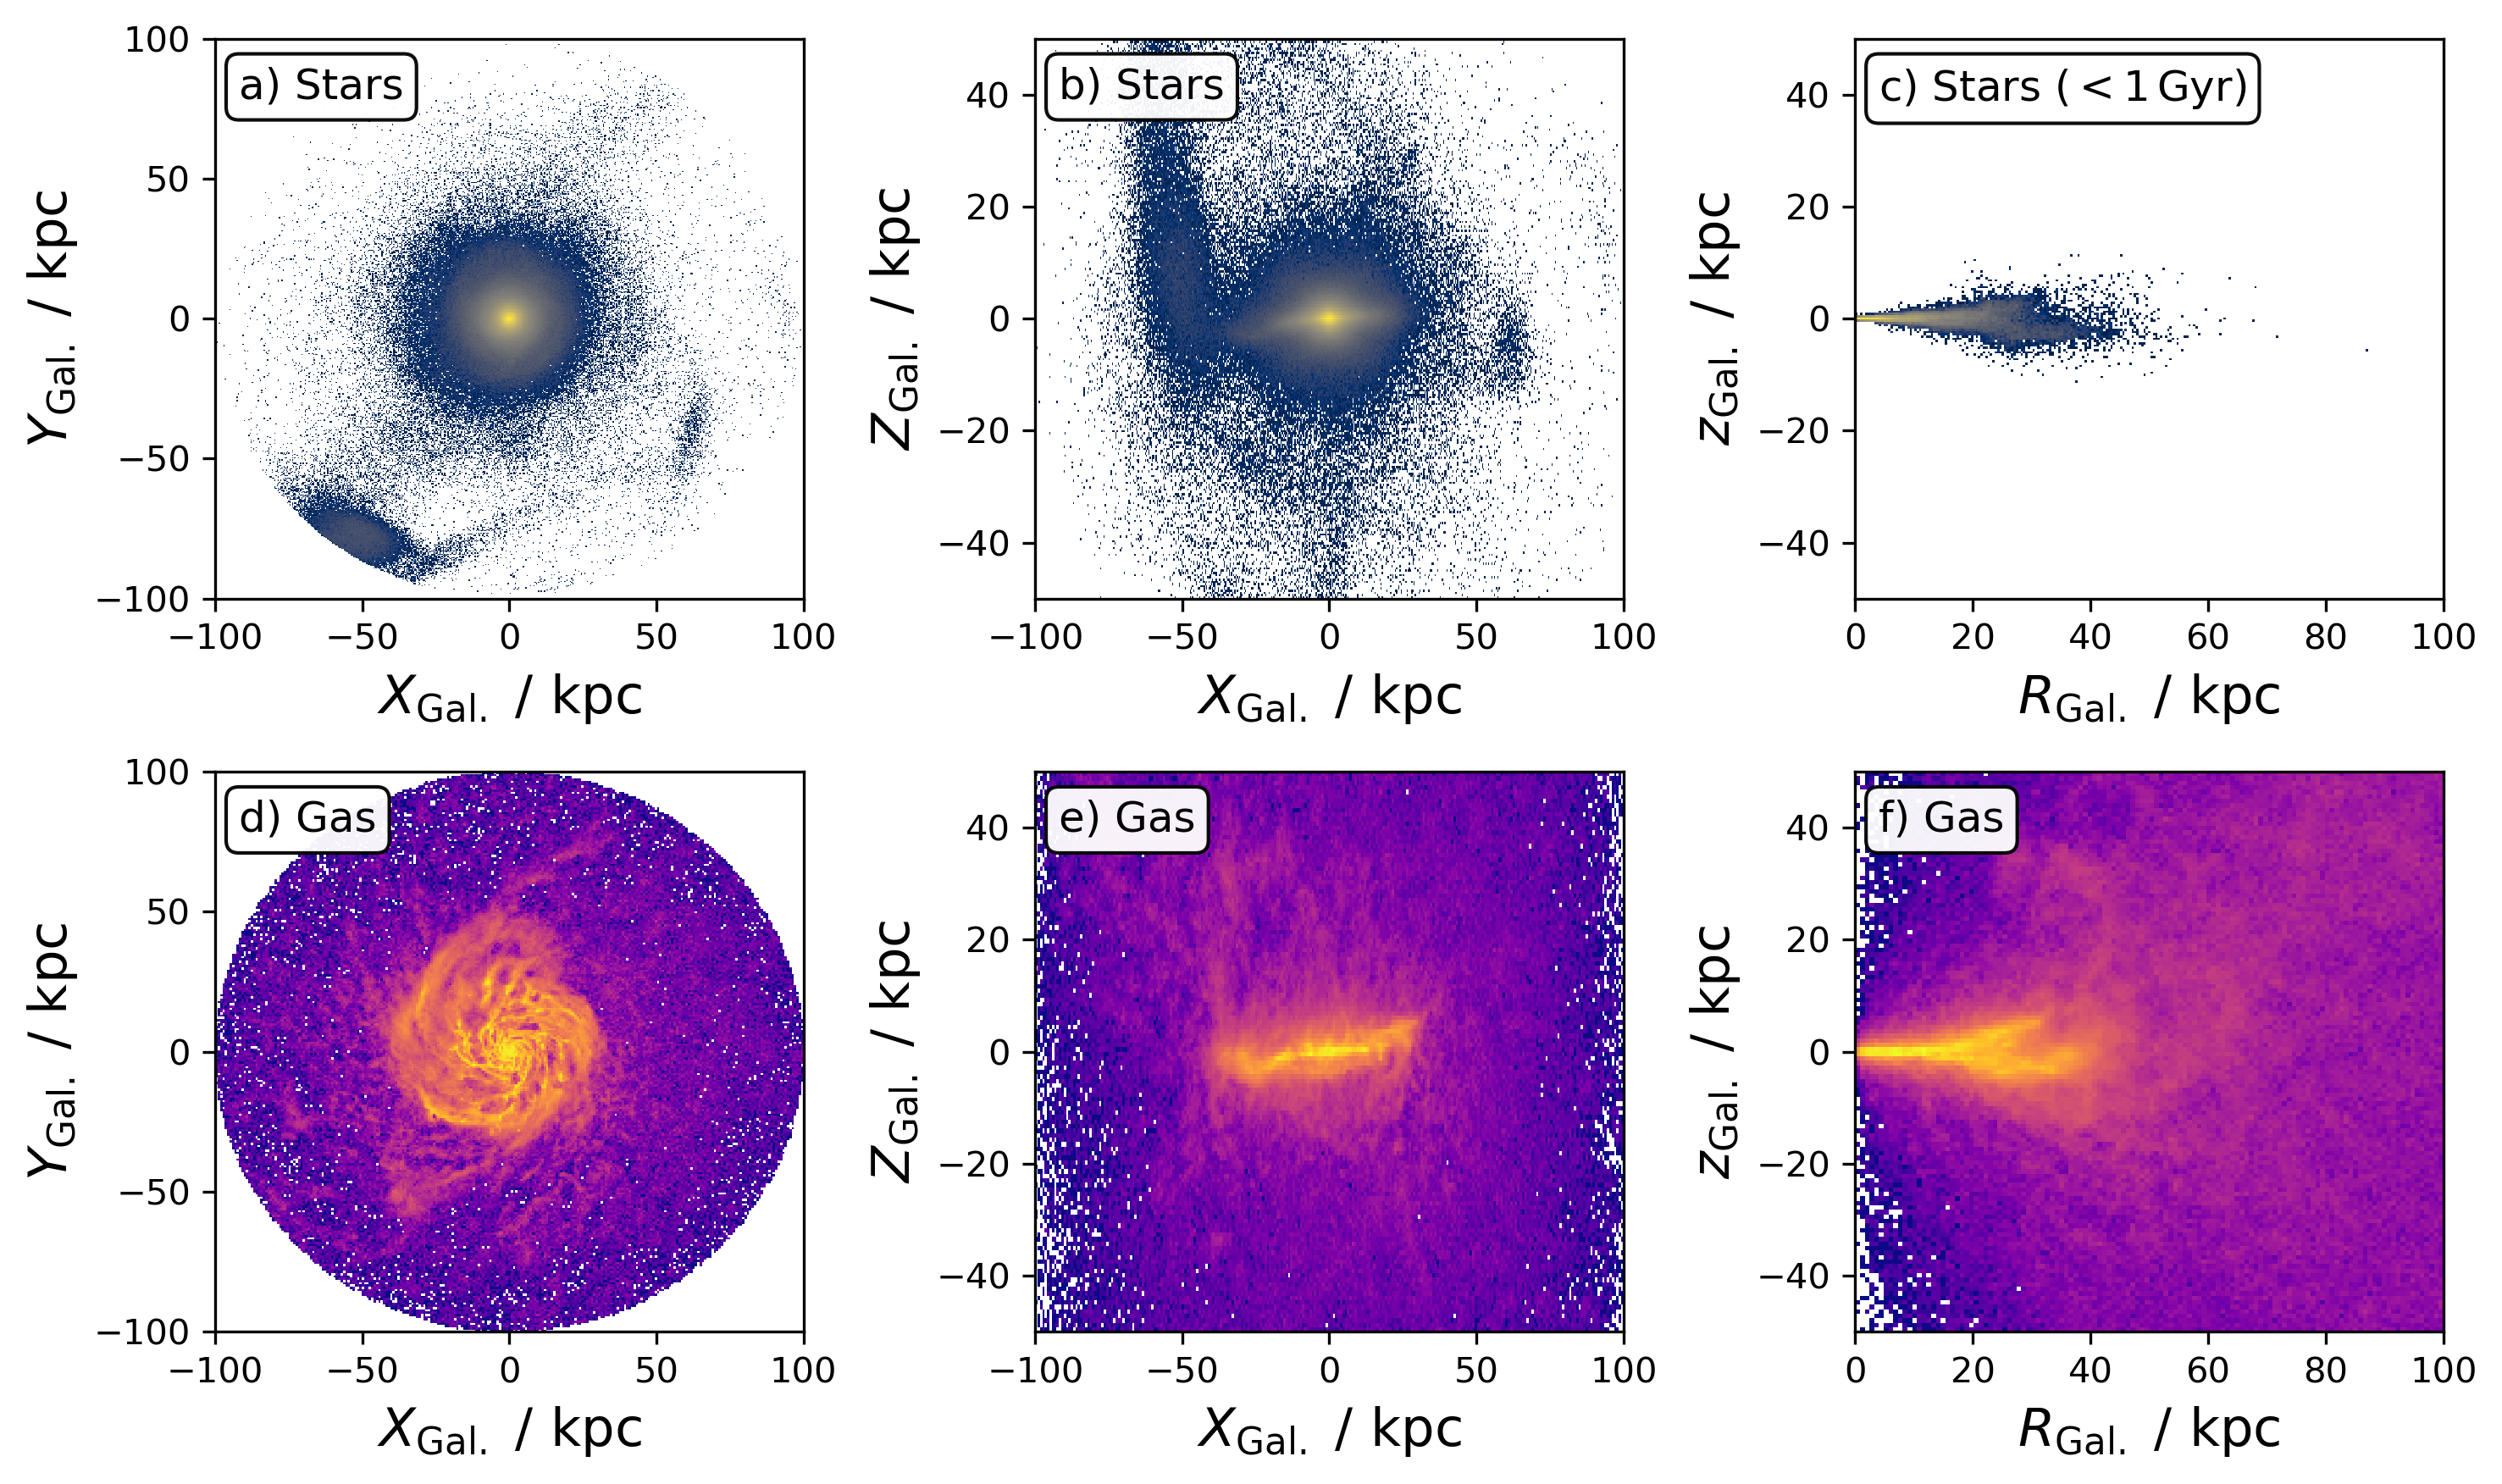
\includegraphics[width=\textwidth]{figures/stars_and_gas_overview_100kpc.png}
    \caption{Same as Fig.~\ref{fig:stars_and_gas_overview}, but for an extended $R_\mathrm{Gal.} \leq 100\,\mathrm{kpc}$ and $\vert z_\mathrm{Gal.} \vert \leq 50\,\mathrm{kpc}$.}
    \label{fig:stars_and_gas_overview_100kpc}
\end{figure*}

Figs.~\ref{fig:tracing_fe_h_young_stars_in_angles} and \ref{fig:tracing_fe_h_residuals_young_stars_in_angles}

\begin{figure}
    \centering
    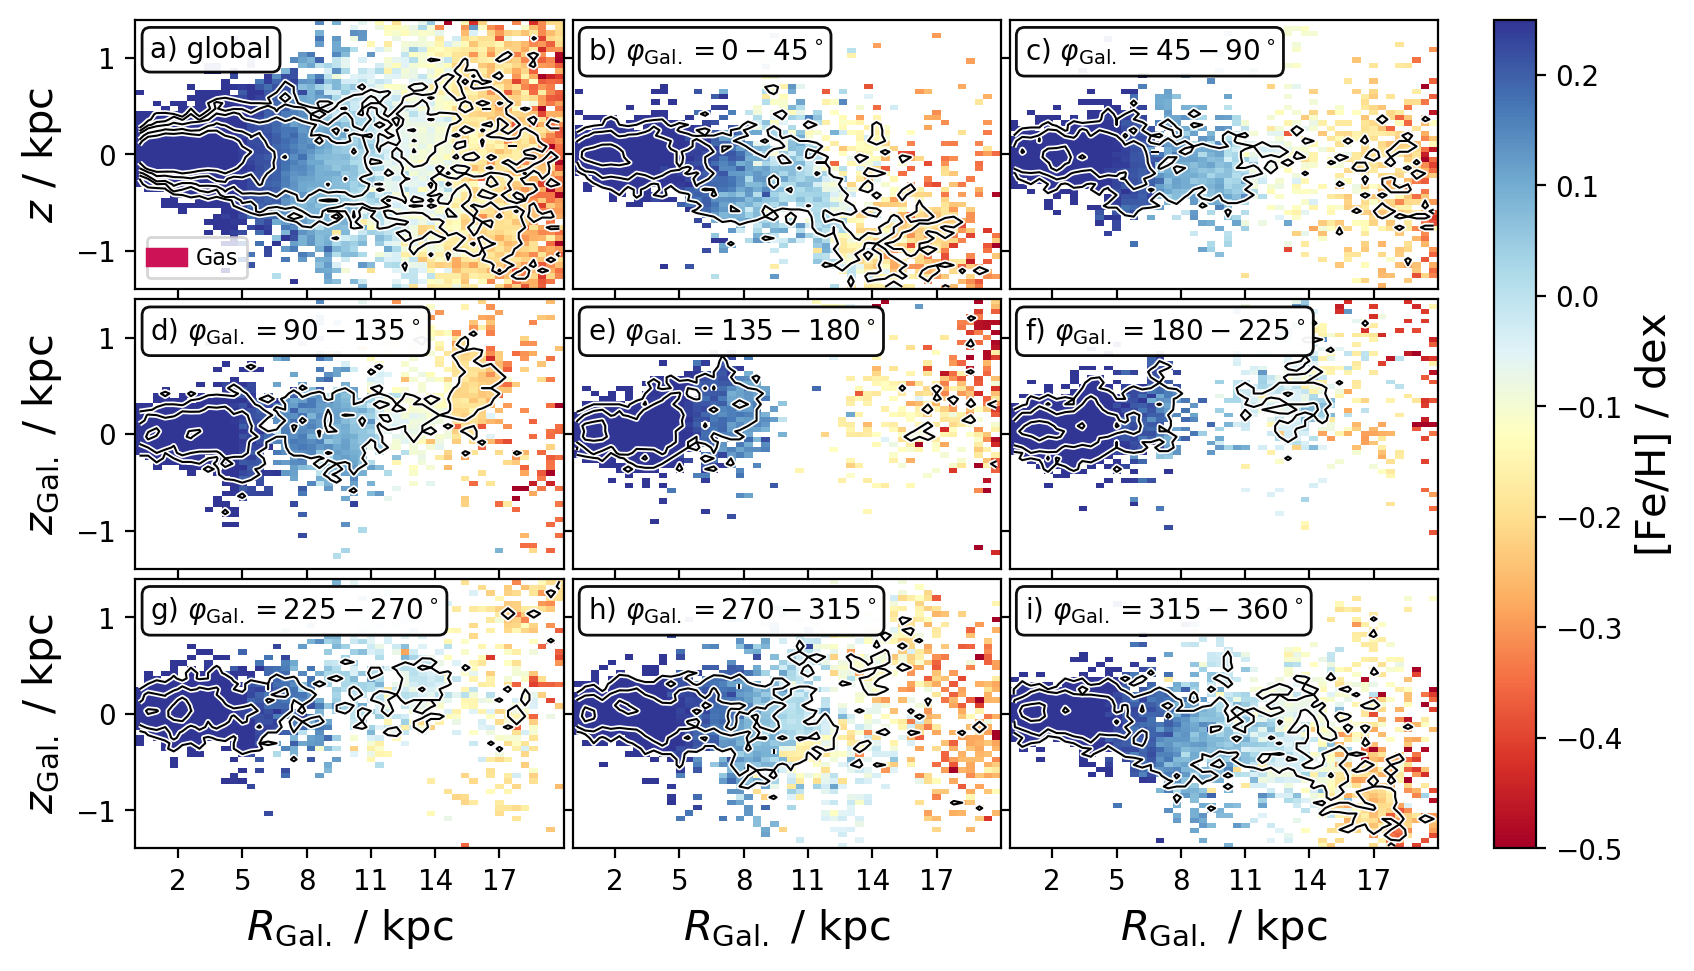
\includegraphics[width=\columnwidth]{figures/tracing_fe_h_young_stars_in_angles.png}
    \caption{Tracing young stars' iron abundance [Fe/H] across galactocentric radii $R_\mathrm{Gal.}$ and height $z_\mathrm{Gal.}$ across the whole galaxy (panel a) and different azimuthal ranges/sectors (panels b-i).}
    \label{fig:tracing_fe_h_young_stars_in_angles}
\end{figure}

\begin{figure}
    \centering
    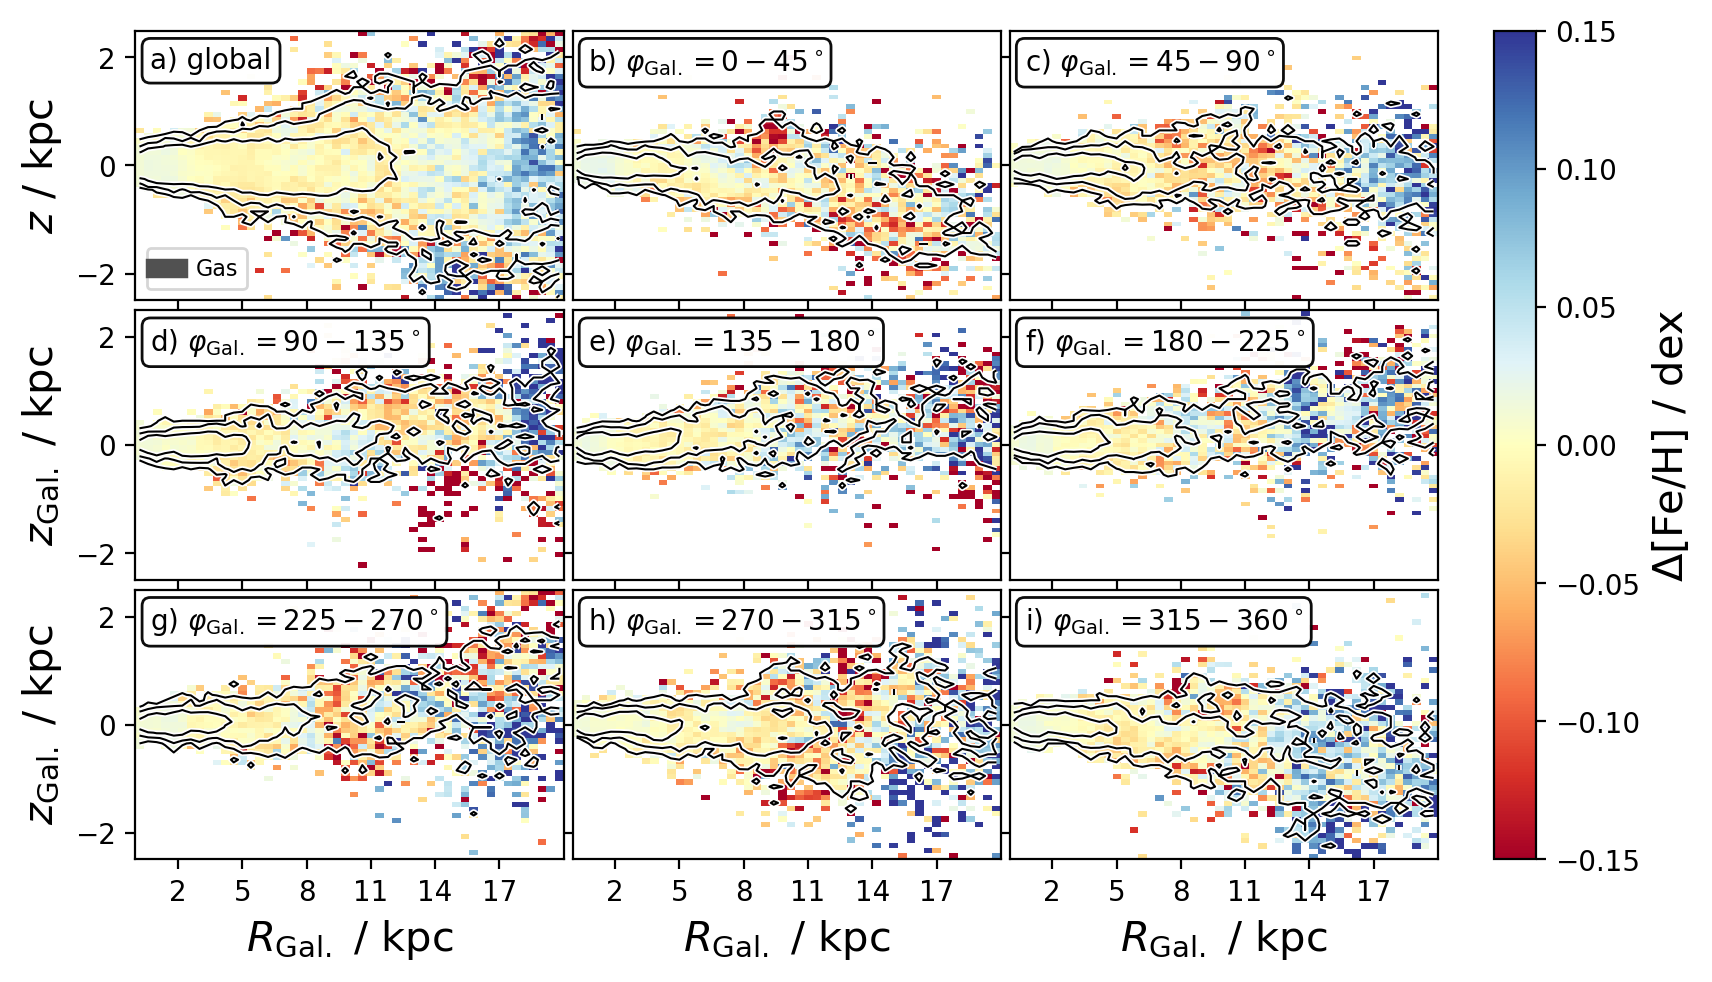
\includegraphics[width=\columnwidth]{figures/tracing_fe_h_residuals_young_stars_in_angles.png}
    \caption{Tracing young stars' iron abundance [Fe/H] residuals (relative to global gradient) across galactocentric radii $R_\mathrm{Gal.}$ and height $z_\mathrm{Gal.}$ across the whole galaxy (panel a) and different azimuthal ranges/sectors (panels b-i).}
    \label{fig:tracing_fe_h_residuals_young_stars_in_angles}
\end{figure}

Fig.~\ref{fig:quadratic_fit_across_ages}

\begin{figure}
    \centering
    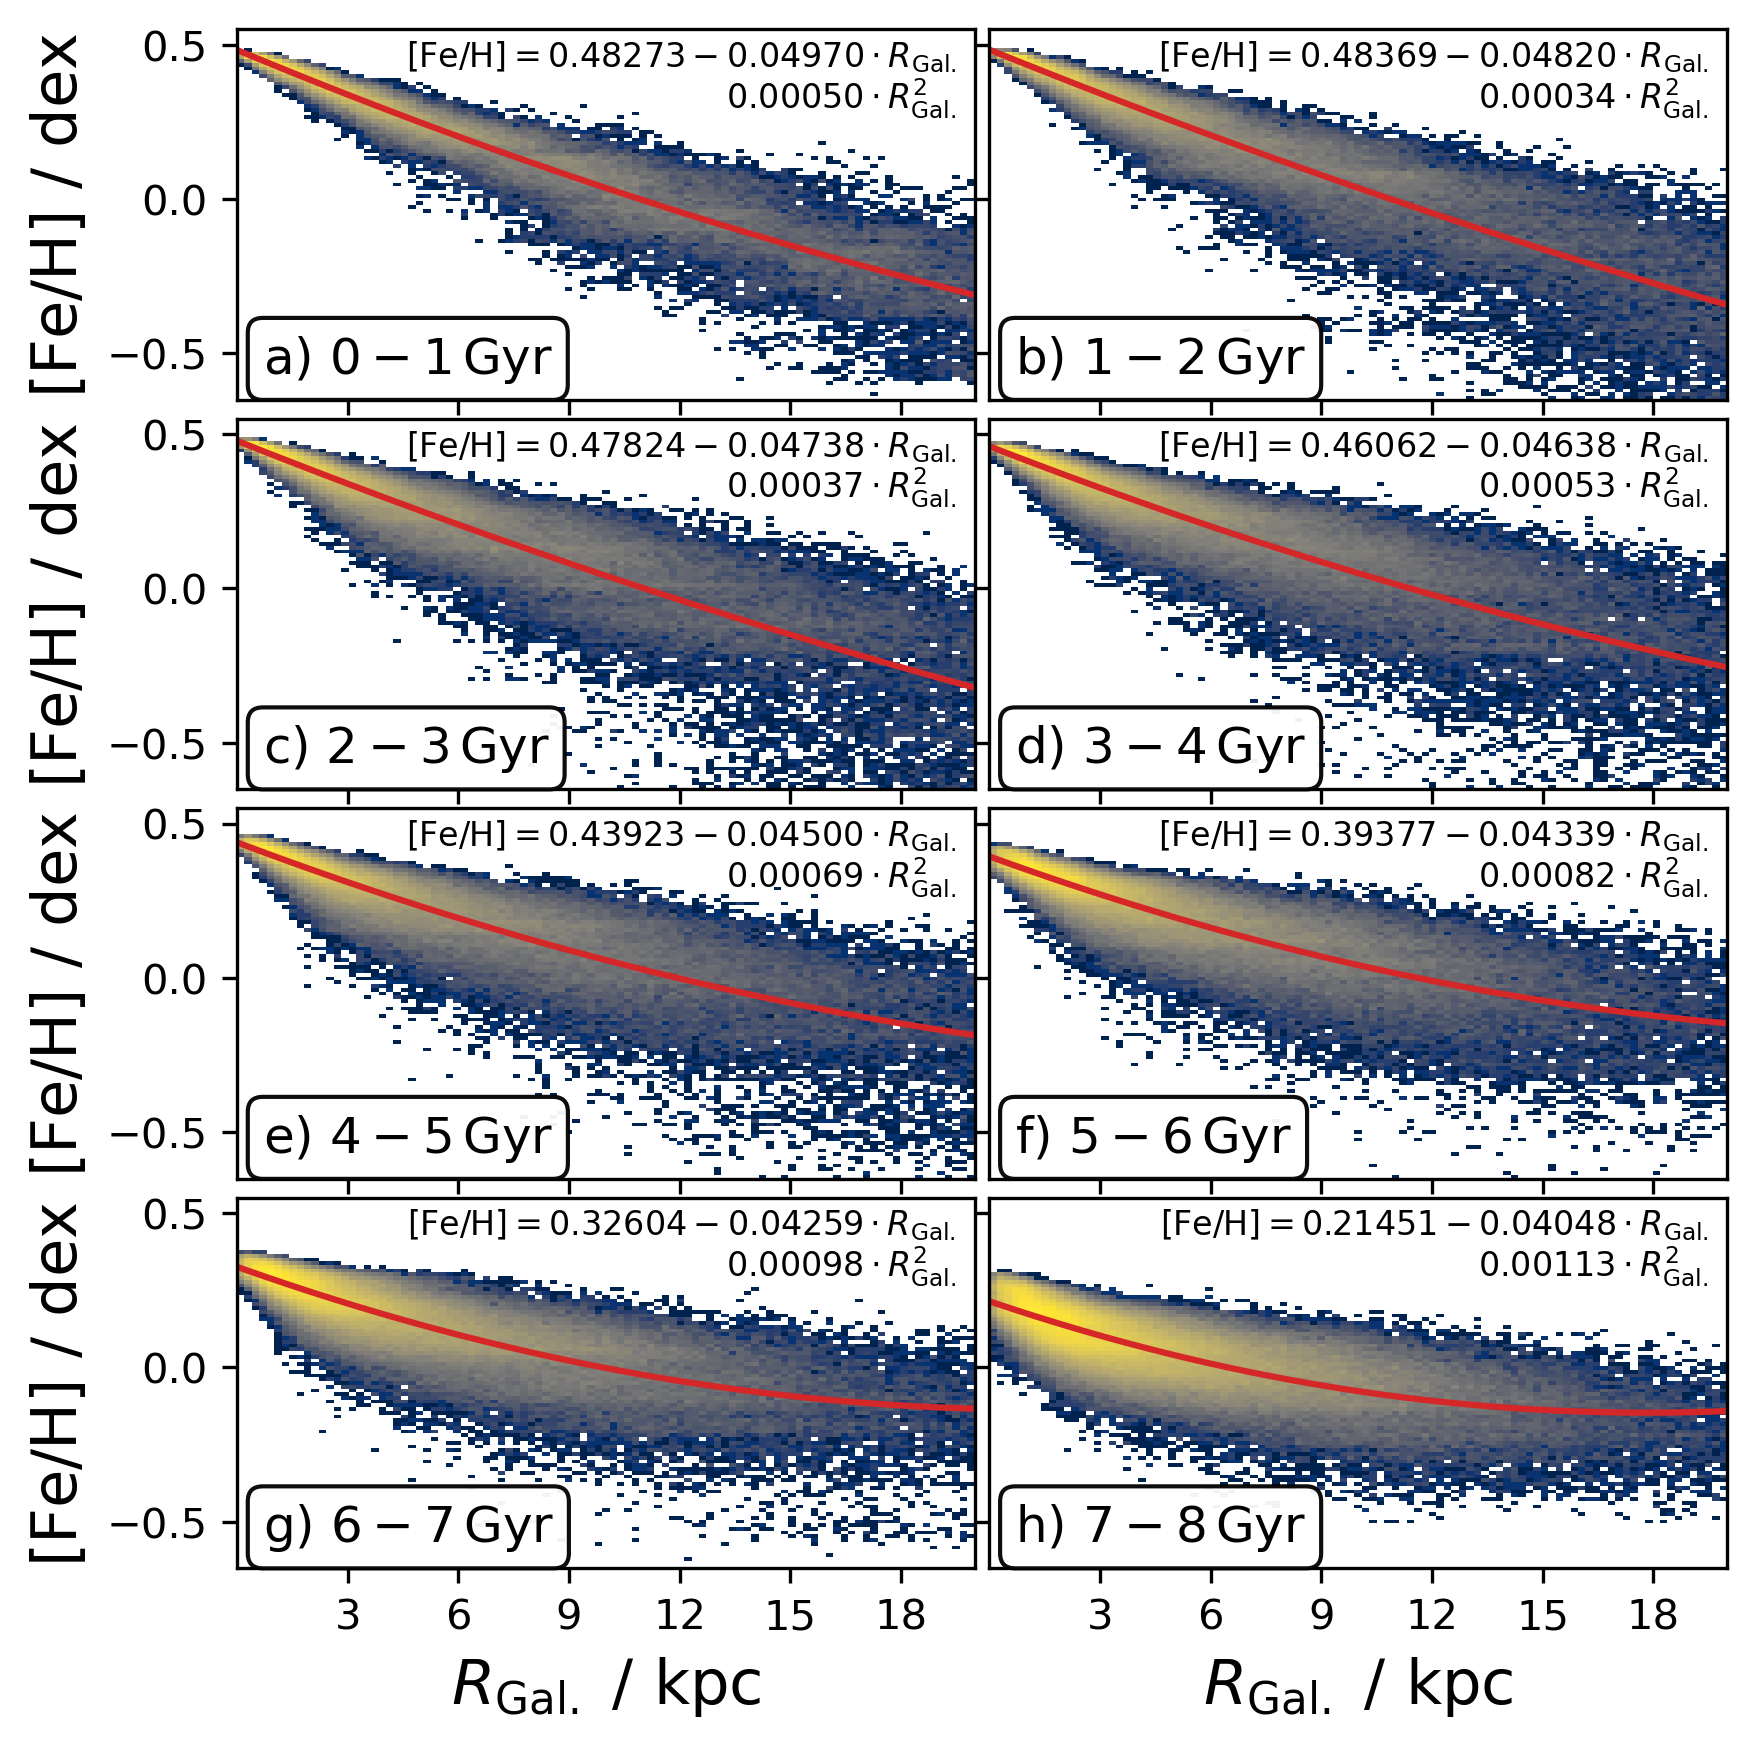
\includegraphics[width=\columnwidth]{figures/quadratic_fit_across_ages.png}
    \caption{Radial metallicity gradients and quadratic fits for $1\,\mathrm{Gyr}$ age bins.}
    \label{fig:quadratic_fit_across_ages}
\end{figure}


%%%%%%%%%%%%%%%%%%%%%%%%%%%%%%%%%%%%%%%%%%%%%%%%%%
% Don't change these lines
\bsp	% typesetting comment
\label{lastpage}
\end{document}